\documentclass[10pt,oneside]{memoir}
\usepackage{layouts}[2001/04/29]
\makeglossary
\makeindex

\def\mychapterstyle{default}
\def\mypagestyle{headings}
\def\revision{}

%%% need more space for ToC page numbers
\setpnumwidth{2.55em}
\setrmarg{3.55em}

%%% need more space for ToC section numbers
\cftsetindents{part}{0em}{3em}
\cftsetindents{chapter}{0em}{3em}
\cftsetindents{section}{3em}{3em}
\cftsetindents{subsection}{4.5em}{3.9em}
\cftsetindents{subsubsection}{8.4em}{4.8em}
\cftsetindents{paragraph}{10.7em}{5.7em}
\cftsetindents{subparagraph}{12.7em}{6.7em}

%%% need more space for LoF numbers
\cftsetindents{figure}{0em}{3.0em}

%%% and do the same for the LoT
\cftsetindents{table}{0em}{3.0em}

%%% set up the page layout
\settrimmedsize{\stockheight}{\stockwidth}{*}	% Use entire page
\settrims{0pt}{0pt}

\setlrmarginsandblock{1.5in}{1.5in}{*}
\setulmarginsandblock{1.5in}{1.5in}{*}

\setmarginnotes{17pt}{51pt}{\onelineskip}
\setheadfoot{\onelineskip}{2\onelineskip}
\setheaderspaces{*}{2\onelineskip}{*}
\checkandfixthelayout

\usepackage{fontspec}
\setromanfont[Mapping=tex-text]{Palatino}

\usepackage{fancyvrb}			% Allow \verbatim et al. in footnotes
\usepackage{graphicx}			% To include graphics in pdf's (jpg, gif, png, etc)
\usepackage{booktabs}			% Better tables
\usepackage{tabulary}			% Support longer table cells
%\usepackage[utf8]{inputenc}		% For UTF-8 support

% \usepackage[T1]{fontenc}		% Use T1 font encoding for accented characters
\usepackage{xcolor}				% Allow for color (annotations)
% diagonal top left cell in tables
\usepackage{slashbox}
% for tables in the appendix
\usepackage[section]{placeins}
\usepackage{geometry}
\usepackage{listings}


%\geometry{landscape}			% Activate for rotated page geometry

%\usepackage[parfill]{parskip}	% Activate to begin paragraphs with an empty
								% line rather than an indent


\def\myauthor{Author}			% In case these were not included in metadata
\def\mytitle{Title}
\def\mykeywords{}
\def\mybibliostyle{plain}
\def\bibliocommand{}

\usepackage{local}

\VerbatimFootnotes
\def\myauthor{Alexy Khrabrov}
\def\baseheaderlevel{1}
\def\format{complete}
\def\latexxslt{memoir-thesis-xelatex.xslt}
\def\mytitle{The Mind Economy of Social Networks: Dynamic Graph Analysis of Communications}


%
%	PDF Stuff
%

%\ifpdf							% Removed for XeLaTeX compatibility
%  \pdfoutput=1					% Removed for XeLaTeX compatibility
  \usepackage[
  	plainpages=false,
  	pdfpagelabels,
  	pdftitle={\mytitle},
  	pagebackref,
  	pdfauthor={\myauthor},
  	pdfkeywords={\mykeywords}
  	]{hyperref}
  \usepackage{memhfixc}
%\fi							% Removed for XeLaTeX compatibility


%
% Title Information
%


\ifx\latexauthor\undefined
\else
	\def\myauthor{\latexauthor}
\fi

\ifx\subtitle\undefined
\else
	\addtodef{\mytitle}{}{ \\ \subtitle}
\fi

\ifx\affiliation\undefined
\else
	\addtodef{\myauthor}{}{ \\ \affiliation}
\fi

\ifx\address\undefined
\else
	\addtodef{\myauthor}{}{ \\ \address}
\fi

\ifx\phone\undefined
\else
	\addtodef{\myauthor}{}{ \\ \phone}
\fi

\ifx\email\undefined
\else
	\addtodef{\myauthor}{}{ \\ \email}
\fi

\ifx\web\undefined
	\else
		\addtodef{\myauthor}{}{ \\ \web}
\fi

\title{\mytitle}
\author{\myauthor}

\begin{document}

\chapterstyle{\mychapterstyle}
\pagestyle{\mypagestyle}


%
%		Front Matter
%

\frontmatter

% Title Page

\titlepage
%\maketitle
\clearpage

% Copyright Page
\vspace*{\fill}

\setlength{\parindent}{0pt}

\ifx\mycopyright\undefined
\else
	\textcopyright{} \mycopyright
\fi

\revision

\begin{center}
\framebox{ \parbox[t]{1.5in}{\centering Formatted for \LaTeX  \\ 
 by MultiMarkdown}}
\end{center}

\setlength{\parindent}{1em}
\clearpage

%
% Main Content
%


% Layout settings
\setlength{\parindent}{1em}

\mainmatter
\begin{abstract}
\label{abstract}
\addcontentsline{toc}{chapter}{Abstract}

\begin{Spacing}{2}


Online social networks are novel mechanisms for distributed interaction that have been enabled by affordable and ubiquitous communications and computing. Facebook has over 500 million members (larger than the US population) and Twitter broadcasts over 100 million ``tweets'' per day, projected to reach a daily 1 billion within a year (compared with about 600 million pieces of mail the USPS handles daily). Social networks are growing in reach and impact but little is known about their structure, dynamics or users' behaviors. New techniques and approaches are needed to study and understand why these networks attract users' persistent attention, and how the networks evolve.


This thesis investigates the questions arising when modeling human behavior in social networks, and its main contributions are:


\begin{itemize}


\item an infrastructure and methodology for understanding communication on graphs;

\item identification and exploration of sub-communities;

\item metrics for identifying effective communicators in dynamic graphs;

\item a new definition of dynamic, reciprocal social capital and its iterative computation

\item a methodology to study influence in social networks in detail, using 

\item a class hierarchy established by social capital

\item simulations mixed with reality across time and capital classes

\item various attachment strategies, e.g.\ via friends-of-friends or full utility optimization

\item a framework for answering questions such as ``are these influentials accidental,'' by performing multiple simulations, with various starting conditions from reality, and seeing how various rules lead to new worlds where the new winners might, or might not, overlap with the real ones, segmenting the factors contributing to success and their randomness or stability




\item discovery of the ``middle class'' of social networks, which is the real influential in many processes, as shown with our new metrics and simulations



\end{itemize}

These methods have already lead to the discovery of ``mind economies'' within Twitter, where interactions are designed to increase ratings as well as promoting  topics of interest and whole subgroups. Reciprocal social capital metrics identify the ``middle class'' of Twitter which does most of the ``long-term'' talking, carrying the bulk of the system-sustaining conversations. We show that this middle class wields the most of the actual influence we should care about --- these are not ``accidental influentials.''  Our approach is of interest to computer scientists, social scientists, economists, marketers, recruiters, and social media builders who want to find and present new ways of exploring, browsing, analyzing, and sustaining online social networks.


\end{Spacing}


\chapter*{Acknowledgments}
This thesis is a synthesis of many years of research and industrial experience, which had begun with my arrival in the United States at the invitation of Prof. George Cybenko of Thayer School of Engineering, Dartmouth College.  Now, coming a full circle, I am a researcher at Thayer again, and a citizen of the United States myself, with the new citizens --- our children Edward and Eva --- added already with my wife Olga (and more on the way).  I want to thank George for the great opportunity he opened, his scientific guidance, and sharing his wisdom and ability to see what's really important.  When working with him, you appreciate how invariably sharp, patient and understanding George is with people in any project he undertakes.  As a great scientist himself with strong computational contributions and a mathematical view of the world, managing multiple large-scale projects without ever losing his cool, George is always the example to follow for me.


I want to thank my new country, the United States of America, for upholding freedom and liberty, leading the world in innovation, and providing people of all backgrounds with amazing opportunities to come together and do great things for the world and each other.  Through its democratic system and appreciation of science and technology, the US enables such great institutions of learning as the University of Pennsylvania and Dartmouth College, and such singular laboratories of the Internet innovation as the Silicon Valley --- where we're headed next.


I thank Professor Emeritus Noah Prywes, one of the founders of the CIS, who gave me my first job at CCCC, one of the oldest computer companies in the US, and recommended me to the CIS program at Penn.  Bonnie Webber was my original Penn advisor.  Her knowledge, focus on medical research applications, and engaging manner illuminated my first year at Penn, and with her I also started working with Curt Langlotz, one of the first MD/PhDs using natural language processing in medical domain --- my first application of functional programming with both academic and industrial impact, a tradition continued throughout my career and in this thesis.   Bonnie had left for Edinburgh and was succeeded by Lyle Ungar. When I took my first AI class with Lyle, I wished this lively guy in plaid shirt could be my advisor --- which did happen, and Lyle had become one of the most engaging scientists I was lucky to work with.  Lyle fuses broad knowledge of data mining and machine learning with very practical approach to problem solving --- and he enables it by being one of the best communicators inside and outside of science I've ever met.  I'm glad he had put up with me through all these years, with so many ideas --- and I'm positive we'll find more areas of collaboration going forward.


My committee is an amazing group of experts in social networks, data mining, and computational linguistics.  Mark Liberman was supportive of my research at Dartmouth and had asked the key question --- are these Accidental Influentials, by any chance? --- which employed our Reciprocal Social Capital metics to the fullest.  Jonathan Smith, the chair, grounds it in all-encompassing computer networking expertise, and Shawndra Hill adds an operational and business perspective which, as you can see, is the most welcome pattern here.


Professor Rajiv Alur, the former graduate chair, has outlined the graduation plan for me to execute at Dartmouth, which I followed.  Professor Jianbo Shi, the current graduate chair, guided it through completion and took the time to listen to the whole presentation in advance, providing insightful feedback.


Alexandrin Popescul and Andrew Schein are steadfast friends and colleagues since the Ph.D. program under Lyle, and now future neighbors, --- with Alex also a colleague again, --- in the Bay Area.  Alex and Andrew provided numerous hours of discussion of the technologies and also their purposes and applications.  Their successful application of data mining in industry is the best use of what Lyle and others had taught us and an example to follow, again.


Val Tannen had first introduced me to ML, which I'm using to this day (and in this thesis extensively).  He and Jean Gallier provided steadfast academic support at Penn, and Norm Badler and Rajiv Alur helped my candidacy come around and track to the plan, keeping the eyes on the prize.  Eduardo Glandt had always made things nicer with his charm, and oversees SEAS and CIS through amazing advances, making it an even better place to graduate from.


My father, Professor Victor Khrabrov, is a physicist and the inventor of the first electric rocket flown into space.  I owe my interests in science and engineering, as well as in Cicero, literature, arts, and much more, to him.  He was always a supreme optimist and was happy to see me following through with my Ph.D.  I hope he'll be proud of me from wherever he is now.  My mother, Anna Khrabrova (Drabkina), was always supportive and believed in me to the extent she'd become a resident of Philadelphia too.  To her, my Penn odyssey had a benefit of my regular visits (by train!), and enjoying Philly together, including its great classical orchestra at the beautiful Kimmel Center.  I have to thank the city of Philadelphia here, for being a home city, a social network enabling science and creativity and inseparable from the Penn experience.  Dartmouth, as my first home in the US, and then our first long-term family home, is also a special place like no other.  (Snowshoeing!)


Dmitri Levonian, a founding partner at Renova Capital (now Svarog Capital Advisors), is a rare example of a deep thinker and successful financier who can implement his vision via scaling a global business.  Working with him I got a chance to attend to all aspects of an R\&D enterprise, go together to the Machine Learning Summit in Copenhagen, and do focused computational research of English and Russian.


My friends and colleagues at Amazon.com, notably Dean Kassmann, Chris Jones, Ryan Rawson, and Jacob Nelson, taught me that you can --- and should! --- apply advanced concepts in process control, supply chain management, personalization, and functional programming to reality at scale to improve productivity and do better.


Peter Yianilos has brought me to the NECI, with the startup idea of a global, eternal, indestructible Intermemory -- whose time is still to come one day.  Peter is awesome, and can make things clear simply by the tone of his voice; his math skills are a stellar match to his pioneering business record, and overall he is a great example to follow.  The team at NECI included Lee Giles, a father figure to us all, Steve Lawrence (now at Google) and Dave Pennock (now at Yahoo Research), all great friends.  Gary Flake went on to found and lead industrial labs at Yahoo and Microsoft, showing how to scale serious research in practice.


The teams at Google, Microsoft, Efficient Frontier, and TopProspect had all shown interest in the research presented here.  I've chosen the latter, for its startup spirit and vision, but I respect all of them and see them as my future colleagues in the field of practical social network mining.


In closing, I have to mention those whom I always remember --- my grandfathers who fought in the World War II and defended our lives.  My paternal grandfather, Alexander Khrabrov, was lost in action in 1941, defending Moscow.  My maternal grandfather, Semion Drabkin, had become a war hero, delivering the ultimatum at Stalingrad, personally capturing Nazi criminals who testified at Nuremberg, liberating cities, and working together with the Allies in the denazification of Germany.  He went on to become a chief missile designer, --- but it were his grandsons, not his missiles, which ended up in the US.  His perseverance at Stalingrad had inspired my own through the Ph.D. process.


\pagebreak 
\end{abstract}
\clearpage
% Table of Contents
\tableofcontents
\clearpage
\listoffigures			% activate to include a List of Figures
\clearpage
\listoftables			% activate to include a List of Tables
\clearpage


\chapter{Introduction}
\label{introduction}

\begin{Spacing}{2}


On March 25th, 2011, ``The Fifth Down,'' an NFL blog of the New York Times, opened as follows \cite{tanier2011ochocinco}.


\begin{quote}
An independent research company called Twitalizer ranked Bengals wide receiver Chad Ochocinco as the second-most influential personality on Twitter, according to David Leonhardt's article on The 6th Floor blog on Thursday.


Ochocinco ranks behind the Brazilian comedian Rafinha Bastos. He ranks well ahead of President Obama, Justin Bieber, Oprah Winfrey, Sarah Palin, and yes, Charlie Sheen. Twitalizer doesn't just track followers (Lada Gaga and Bieber have the most), but ``mentions'' and other criteria that determine who is making real contributions to the discussion.


Leonhardt's article barely mentions Johnson --- he appears in the top-ten list --- but the football world quickly picked up the story of his influence. Let's face it, we do not have much else to do. What makes Johnson more influential than, say, Terrell Owens or Aaron Rodgers, let alone Bieber or Palin? Take it from a longtime Chad Johnson/Ochocinco psychoanalyst: the recipe for Internet domination is simple.
\end{quote}


Written off season, during an NFL lockout, this column indicates the reach of social networks, their mainstream appeal, and the fact that many people care about influence in such networks.


How did we end up here?  What can it possibly mean to ``have influence'' in a ``social network''?  Did Chad Ochocinco get to the top by accident, or does he deserve to be there?  These are the key themes of this thesis.


\pagebreak \section{Overview}
\label{overview}

Modern human society is first and foremost a society of the mind --- a social mind, a new collective ecosystem self-organizing and communicating via the Internet, as well as comprehending itself and organizing various collective actions.  The thought becomes action after reaching a critical mass of actors.   A concept which becomes action goes through a lifecycle of invention, being noticed by the influencers, spreading, taking hold, and crossing some sort of a phase transition.  A telling feature of any successful idea is its transition from individual to group to global level in the network.  Determining these levels and detecting how people and ideas relate to them is key to understanding network dynamics.


Spreading news, knowledge and ideas, arguing about them, and forming groups around them has always been the essence of culture. Political thinkers and rules, artists, and philosophers are examples of the original social networks which circulated relevant knowledge and made a discourse out of it.


In a situation where concepts are tangible as reproducible units and can be retranslated, they take on qualities of currency.  For instance, the concepts underlying the backbone of the Internet itself relate to code, and in recent years we saw a dramatic rise in social coding via social coding networks such as {\itshape github}, {\itshape bitbucket.com, \_patch-tag.com}, etc.  Code ideas are often expressed as working snippets (gists) and contain URLs to use and run right away.


When ideas' traction is quantifiable and idea exchanges lead to measurable change in ranking of both actors and goods being exchanged, an economy inevitably evolves, which we call the Mind Economy and to the study of which we devote this thesis.


Our Mind Economy study focuses on the fundamental questions of communication on a network, the goals of each actor and group of actors, and understanding the nature of influence.  Simply put, we want to know


\begin{itemize}


\item why do people twitter?

\item who has influence on Twitter? 

\item is there a social capital formulation which captures most of people's utilities?

\item can we characterize people by their influence and the types of social behaviors related to attaining it?
\end{itemize}

Since online social networks are driven by software and strongly depend on the algorithmic underpinnings, and produce large volumes of data, a computational approach is required for large-scale data mining.


\pagebreak \subsection{Accidental Influentials}
\label{accidentalinfluentials}

In their seminal 1955 book ``Personal Influence,'' Katz and Lazarsfeld \cite{katz1955influence} proposed the concept of influentials in social networks, propagating and filtering media streams in their communities.  Watts and Dodds, in their own 2008 paper, popularly known as ``Accidental Influentials,'' had shown that for a diffusion model with cascades, it's not necessary to have influentials to excite a typical network.  A Twitter study co-authored by Watts shows that influentials are not propagating URLs much better than the rest of us.  So are these influentials indeed accidental?


We look at a basic form of influence, showing how effective a communicator a person is in the social network.  We use our own reciprocal social capital as a metric keeping track how a person prioritizes his or her replies, paying attention to ``communication balances'' owed and to whom -- e.g., answering questions of somebody with a high social capital more often.  Any such metric induces a ranking among the users, and we build a class system on top of this ranking, resembling a human hierarchy of wealth.


In the US, top 1\% of population by wealth has 35\% of all net worth, while top 10\% has 63\%.  The second 10\% of people has 12\% of net worth, and the bottom 80\% have only 15\%.  Figure~\ref{figure:us-net-worth-hierarchy} is taken from  G. William Domhoff, a professor at UCSC and the author of ``Who Rules America'' \cite{domhoff2006rules}, keeping track of these statistics over the years, now in its 6th edition.  His web site, \url{whorulesamerica.net} \cite{domhoff2011whorules}, contains many instructive graphs segmenting the wealth hierarchy in the US and other countries.  They follow the same law, with different exponents.  Figure~\ref{figure:us-fin-wealth-hierarchy} shows financial wealth, which is the net worth without the real estate used by the owners, comprising the bulk of the middle class equity.


Such division causes emotional reactions.  Bob Herbert, an almost 18 years columnist for the New York Times, cites these statistics as follows in his March 26, 2011 column ``Losing Our Way'':


\begin{quote}
There is plenty of economic activity in the U.S., and plenty of wealth. But like greedy children, the folks at the top are seizing virtually all the marbles. Income and wealth inequality in the U.S. have reached stages that would make the third world blush. As the Economic Policy Institute has reported, the richest 10 percent of Americans received an unconscionable 100 percent of the average income growth in the years 2000 to 2007, the most recent extended period of economic expansion.
Americans behave as if this is somehow normal or acceptable. It shouldn't be, and didn't used to be. Through much of the post-World War II era, income distribution was far more equitable, with the top 10 percent of families accounting for just a third of average income growth, and the bottom 90 percent receiving two-thirds. That seems like ancient history now.
The current maldistribution of wealth is also scandalous. In 2009, the richest 5 percent claimed 63.5 percent of the nation's wealth. The overwhelming majority, the bottom 80 percent, collectively held just 12.8 percent.
\end{quote}
Herbert ends his column (as this text and as a series) to address the imbalance:
\begin{quote}
This is my last column for The New York Times after an exhilarating, nearly 18-year run. I'm off to write a book and expand my efforts on behalf of working people, the poor and others who are struggling in our society.
\end{quote}


While policy opinions differ on what to do with such distributions, there are many such hierarchies in nature and society, caused by many factors.  In economics, such distributions are commonplace, and we use a Zipfian hierarchy when modeling the distribution of social capital wealth.



\begin{figure}[ht]
\minipage[b]{0.5\linewidth}
    \centering
    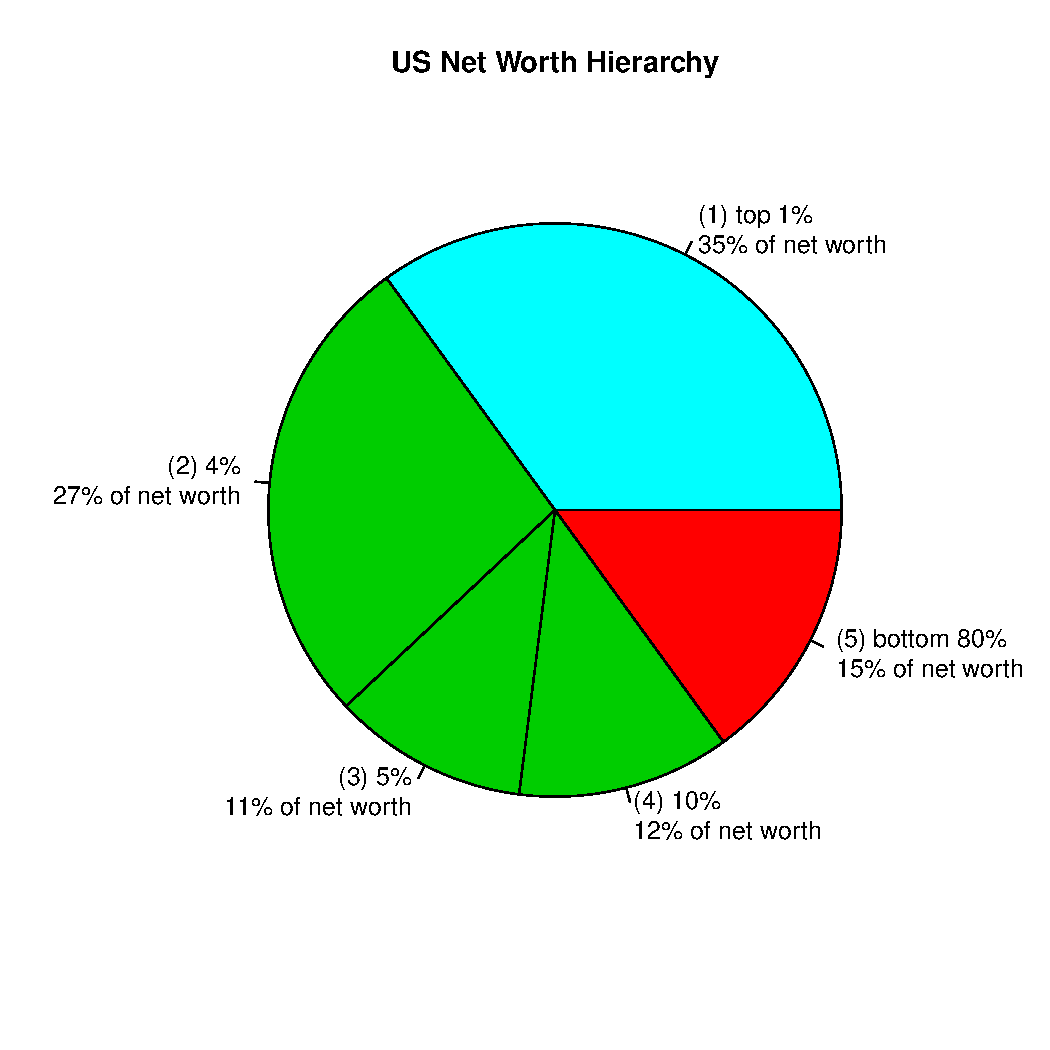
\includegraphics[scale=0.5]{figures/us-net-worth-pie}
    \caption{A small percentage owns the majority of US net worth}
    \label{figure:us-net-worth-hierarchy}
\endminipage\hfill%
%
\minipage[b]{0.5\linewidth}
    \centering
    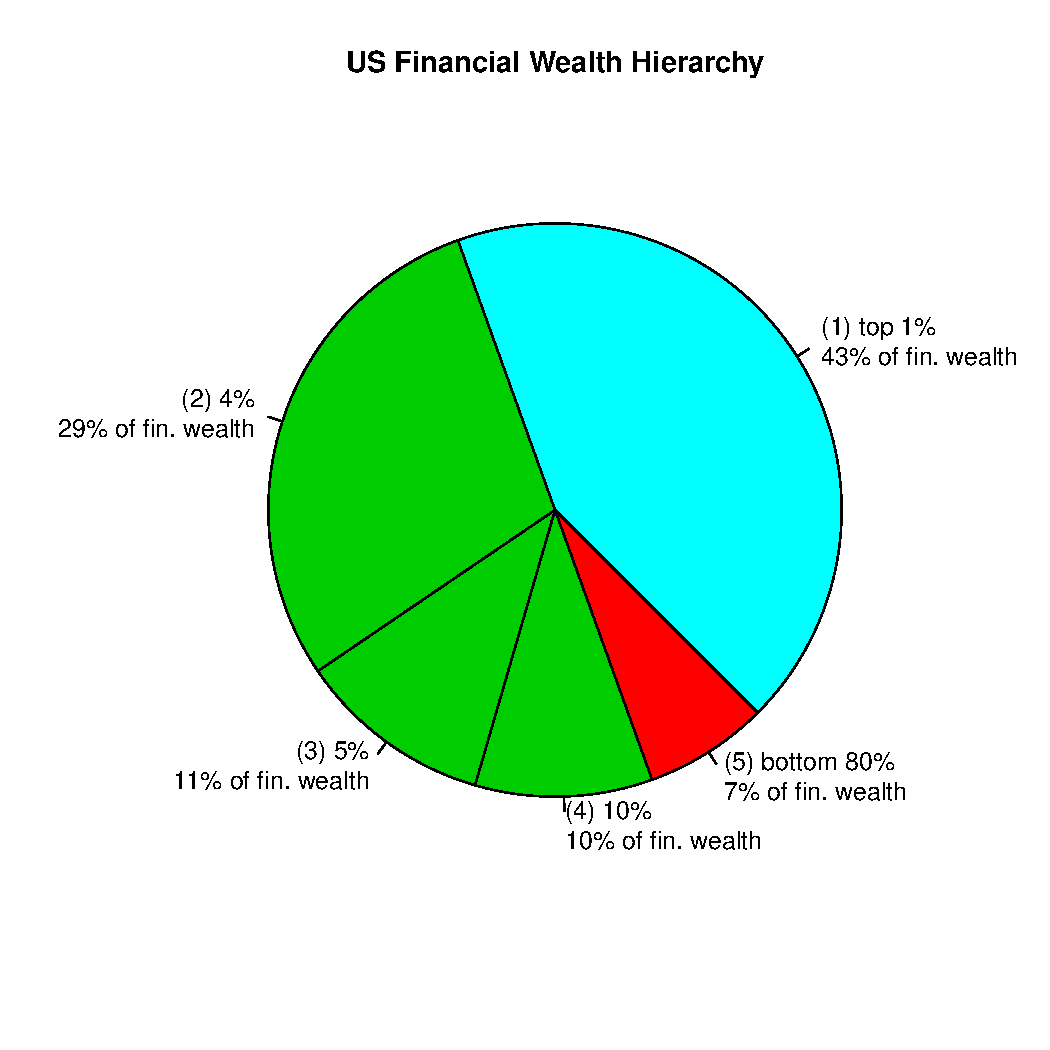
\includegraphics[scale=0.5]{figures/us-fin-wealth-pie-5pm}
    \caption{A small percentage owns the majority of US financial wealth, following the Zipf law.}
    \label{figure:us-fin-wealth-hierarchy}
\endminipage
\end{figure}
In order to see whether the influence hierarchy is random or not, we simulate many parallel worlds, where users talk to each other based on various global and local optimization criteria.  Some of these criteria are simple, such as attaching randomly, or proportionally to the global in-degrees; some are complex, such as attach to a friend of a friend proportionally to their own mentions or social capital; or, ultimately, optimize your local capital gain locally, using the same reward function which is the foundation of the final ranking.  We either simulate the new worlds from scratch, or seed them with a few weeks of the real dynamic graph.  In all cases, we preserve the order of users joining the network and their out-degrees for each day.


Having built the dynamic hierarchy of influencers, changing daily within its own world, we compare the winners in the corresponding positions with the real ones, and across the worlds.  We look at the staying power in the same class bucket across days within the same world, and overlap of the respective buckets across different instances of the same world type, seeded with different lengths of reality to obtain week-shifted ones, or across different worlds altogether.


We observe that the more intelligent a simulation is, the higher is its staying power, showing that the influencers -- those in the higher classes -- are not random in their own worlds.  The overlap of the simulated influencers with the real-world ones is minimal, but also increases with more intelligent attachment strategies.


Our conclusions are as follows.


\begin{itemize}


\item the influentials are not random in their own worlds -- they correspond best to what the attachment strategies are the common rules in these worlds, but they are also those nodes who were well-positioned in their network to take advantage of these rules.  For instance, a global uniform attachment leads to the same stable celebrity bucket (the top one), even though the rest are churning through.  These celebrities stay very stable during the lifespan of their world, but are totally different across various runs of the uniform world.  At the same time, top buckets of smarter simulations show overlaps higher than 50\%, more than overlap of any other two simulations, showing that their success under the rules of those worlds is repeatable even when many edges are rearranged, and thus is not random.




\item the non-bucketed overlap with the real winners is small, proving that the winners in this world are lucky to have the set of rules which distinguished them.  If the accepted attachment strategies were slightly different, others would easily replace the current winners in some of the top buckets, and stay there under wide ranges of new conditions and their combinations.  In that sense, if we agree that our world with its own communication rules is itself random in a series of many similar ones where such rules can be slightly altered, the influencers might indeed be accidental.   Also, real celebrities may not be approximated by any of our strategies --- while we simulate the middle class quite well.




\item simply prescribing a desirable distribution of influence from the real world, as we do with {\itshape creps} simulations, leads to a stable and reproducible middle class.  It shows that order leads to a stable economy.




\item the middle and upper middle classes of social networks are less random across the more intelligent simulations.  The middle class of social networks is the main discovery of this thesis.  It carries 40\% of all communications, while comprising (roughly) only 20-25\% of population.  These users are the actual majority influencers, and they got where they are due to a diligent attention to communication, its priorities, dynamics, and energy demands.  In that sense, we conclude that success is earned.




\item bucketed simulations allow tracking how composite strategies apply to separate classes, or any combination of classes, either preserved or simulated.




\item the middle class is the real influencer, and it is anything but accidental.  For the kinds of effects which matter, these are the real non-accidental influentials we should care about.



\end{itemize}

Figure~\ref{figure:heatmap-srates-medians-3wk} shows how several groups of simulations, loosely corresponding to either Katz-Lazarsfeld or Watts-Dodds models, relate to reality and each other.  Our social-capital based models, taking into account many features of influencers as effective communicators, end up close to each other and reality, as compared to many simpler simulations, based on either uniform, or mentions-based attachment, such as the simulations of Watts-Dodds.



\begin{figure}
\begin{center}
    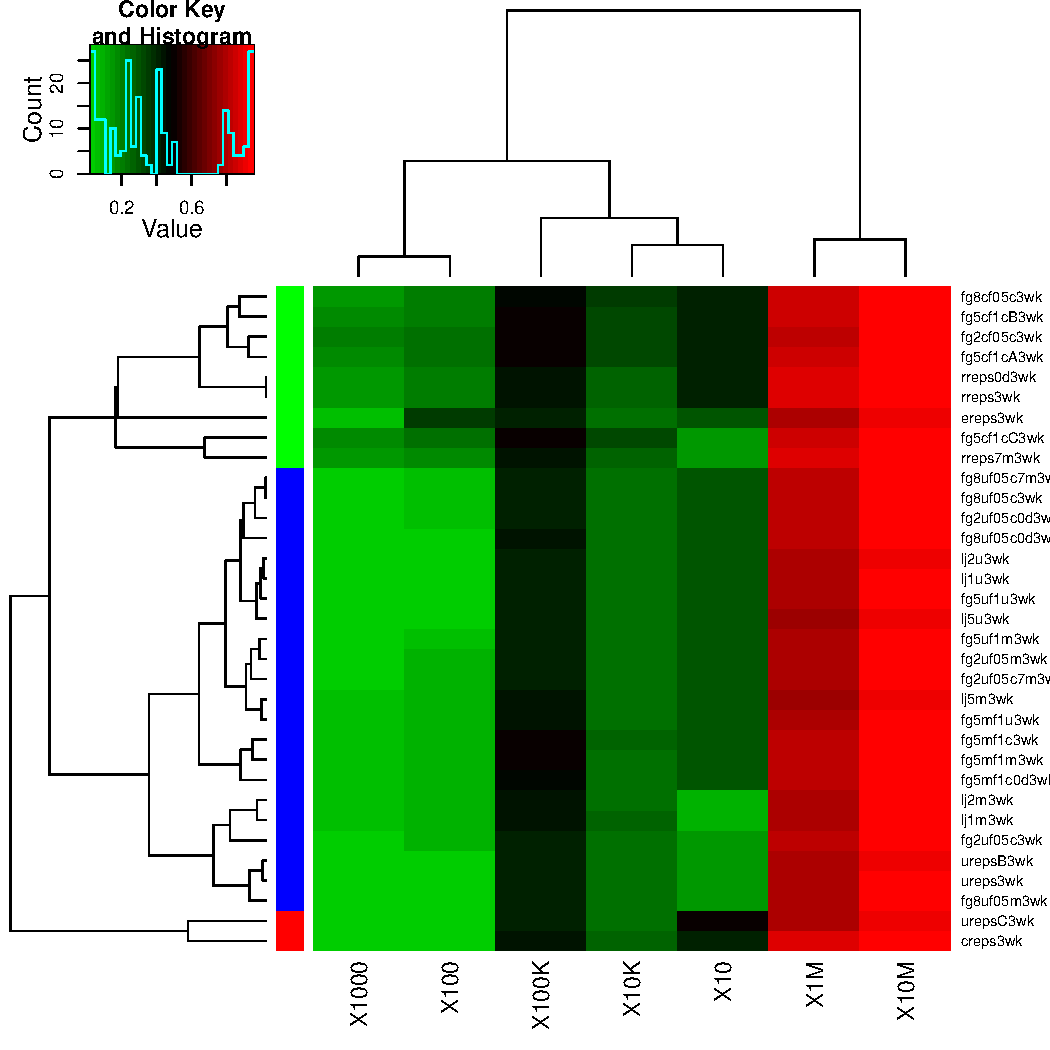
\includegraphics{figures/heatmap-overx-dreps-medians-3wk}
    \caption{Clustering of all simulations seeded by 3 weeks of reality, by overlap with reality.  \emph{Dreps}, the reality itself, ends up closer to our most intelligent capital-based worlds (red), including the simulated middle class.  Simpler networks, including those using only global attachment strategies, end up in a more distant cluster.}
    \label{figure:heatmap-srates-medians-3wk}
\end{center}
\end{figure}
\pagebreak \section{History}
\label{history}

Social networks exist in some form for as long as human society itself.  What made them subject to our computer treatment is their current online incarnation, whereby their operation is code-based, algorithmically guided, and their data is available in bulk for serious data mining.
History of social networks is rich and eventful --- in fact, just like human history itself, which can be considered as an evolution of the kinds of social networks humans organize into, such as tribes, businesses, guilds, classes, nations.


The first recorded blogger, in our analysis, is Cicero.  While he stayed in Rome, engrossed in the politics of the failing Republic he used to uphold as a consul, his epicurean friend Atticus removed to Athens, following Epicurus' maxim that one has to stay away from politics in order to be happy (among other things).  However, Atticus wanted to follow the events back in Rome, and asked Cicero to write him -- almost daily \cite{butler2002cicero}.  According to some accounts, a messenger from Atticus picked up a new letter, often ending with ``you messenger is here so I have to wrap up,'' and delivered it to Athens, where Atticus had a stable of scribes making copies.  The copies were delivered to many prominent Romans all over the Empire for a subscription fee.  That was Atticus' way to enable Cicero to have an income from his talents -- and also spread his influence \cite{phillips1986atticus}.


We see, in Cicero's example, many key features of real influencer in a social network.  When we read Cicero, he comes alive, with all his human emotions, failings, and strengths --- not unlike Chad Ochocinco of today. He has many friends whom he remembers at the right times.  (While most noble Romans had a {\itshape nomenclator} -- a slave who whispered the names of those encountered in the street in their forgetful master's ear -- Cicero needed none.)


Thanks to Atticus, we have a live chronicle of Roman life in Cicero's time, but we also have many letters which Cicero wrote in reply and to maintain his vast social network. Every effective blogger from our online social networks has some, rarely all, qualities which Cicero demonstrates in his own correspondence:


\begin{enumerate}


\item a vast network of contacts

\item engagement with topics of the day and issues of public interest

\item high-intensity writing, frequent and consistent in time

\item engagement with the readers

\item writing for well-defined communities, the political class and the philosophers

\item \label{item:cicero-balance} careful attention to the balance of communications
\end{enumerate}

While we don't have enough data volume to quantify these points for Cicero, we can quantify most of them in online social networks.  Point~\ref{item:cicero-balance} leads naturally to our reciprocal social capital definition (see Section~\ref{chapter:social-capital}).


The first online social network of notice which is still going strong today is \href{http://livejournal.com/}{LiveJournal}\footnote{\href{http://livejournal.com/}{http://livejournal.com/}} (LJ), started by Brad Fitzpatrick in 1999 as a way to for friends to share their dairies and notes online.  It pioneered most of the features of online networks we now take for granted, such as


\begin{itemize}


\item an account for each user with posts along the timeline

\item a mechanism to follow friends, when their updates can be reviewed as a news stream. This predates RSS and is a key feature of LJ.

\item explicit communities. You can create or join a group and then post to it. Communities' membership and posts can be controlled by moderators, e.g.\ be by invitation only, or open for all.

\item Anybody can read anybody else's journal except for the ``friends-only'' or private posts.
\end{itemize}

These features are present, in some form, in any modern online social network.  Communities may not be explicit, such as Twitter, but then some way to self-organize is always found, such as users adding metadata in the form of {\itshape hashtags} (like \texttt{\#clojure} for the community of Clojure fans).


Facebook and Twitter follow up on the basic framework of LiveJournal with their own tweaks. 
 Facebook is generally closed, ensuring the network grows by expressly approved links.  Photo sharing is integrated into Facebook, making it the largest photosharing site in the world.  The closed nature of Facebook ecosystem necessitates in-network applications, using the API.
Twitter limits ``posts,'' to 140 character ``tweets.''  URL shortening and media sharing are supported by a plethora of external services.
Other networks worth mentioning are LinkedIn, Classmates, and various national versions of the above.  E.g., in Russia there're


\begin{itemize}


\item odnoklassniki.ru (classmates, similar to \href{http://classmates.com}{classmates.com}\footnote{\href{http://classmates.com}{http://classmates.com}})

\item vkontakte.ru (``in touch'', analogous to \href{http://linkedin.com/}{LinkedIn}\footnote{\href{http://linkedin.com/}{http://linkedin.com/}}
\end{itemize}

\pagebreak \section{Twitter}
\label{twitter}

Twitter is the key social network of our time, at least as far as the scientific community is concerned.  It's hard to believe now that it all just started in 2006.  Currently Twitter has about a hundred million users worldwide.  When we started getting the gardenhose \ref{StreamingAPI}, a fraction of all tweets, in 2009, we were receiving about 2 million tweets a day; a year later, it was more than 5 million daily.  As opposed to Facebook, Twitter is practically all open to everybody.  (Those using private tweets are a small minority with specific uses, such as explicit chat.)  Anybody can tweet anything to anybody else, given they know their Twitter nickname, such as \texttt{@john}.  The tweet will appear in \texttt{@john}'s stream when he checks his Twitter account.  


Originally designed to be ready for transmission via SMS, each ``tweet'' must fit 140 characters.  A significant portion of all tweets contain an URL, making Twitter the largest ever machine for URL transmission.  Due to the limit, various ``URL shortening'' services exist, creating and maintaining mappings of long actual URLs to shorter, unique ones.  (There's a mechanism in the works for ``official'' URL shortening by their authors.)  Some shortening services, such as \href{http://bit.ly}{bit.ly}\footnote{\href{http://bit.ly}{http://bit.ly}}, use the mapping to track clicks and URL percolation.


Twitter's online nature shines in the way it has become a vehicle for URL percolation.  Trending often spreads across the Internet subcultures.  E.g., many a YouTube phenomena pick their momentum on Twitter.  Multi-stage processes are possible where in-network and external influence alternate.  Justin Bieber, a son of a single mother from Stratford, Ontario, whose fans' mind economy we study in \ref{thepagerankgeneration}, started as a YouTube boy-singer sensation, was discovered by a talent scouting agency and noticed by Usher, the hip-hop star, eventually sang for \texttt{@barackobama}  and broke into mainstream via the People magazine.   Each stage in life of Justin Bieber's ecosystem, or ``beliebers'', is reflected on Twitter.  


Twitter maintains a list of top ten ``trending topics,'' computed by a proprietary algorithm but clearly counting the frequency of mentions with some heavy timing preference to the present.  There are also, added more recently, local trends, per geographic area.  


Twitter translates all kinds of trends -- both in-network, such as {\itshape memes}, and projections of the real world, or rather harsh outside reality, such as \texttt{\#michaeljackson}.  The latter often represent major news, and may be distinguished by multiple, almost simultaneous, injection points.  It can be an interesting project to use the injection dynamics for differentiating the externally induced trends, and perhaps also their strength and globality.


As Mikhail Gronas, a researcher of Russian folklore and global online discourse, noted \cite{Gronas:2010:Private}, Twitter is a global megaphone, or, as we observe, a global echo chamber, which amplifies trending echoes from the outside world, but also has power to process and project them back into the world as Twitter itself grows in influence.


When studying influence, it's important to distinguish between the global mirror and global megaphone behaviors of the network.  It's hard to control for all the externalities on an injected concept.  


Examples where Twitter itself drives reality keep piling up with its growth.  Octavia Nasr, a senior Middle Eastern desk editor for CNN, mentioned her respect for a Lebanese Muslim cleric known, among other things, for his defense of women's rights, and was fired since the cleric was also a polarizing figure in Arab-Israeli relations, so taking sides might have created an appearance of impairing her impartiality.  Dmitri Zelenin, a governor of the Russian Tver region, tweeted a photo from a Kremlin reception showing an earth worm in a plate of salad.  He was reprimanded by a President Medvedev's senior aide, who suggested that the list of ``firable'' offenses for governors should be amended with a cause ``for stupid and irresponsible tweets''.  In fact, President Medvedev of Russia is on the highest level of using Twitter in politics -- he visited Twitter's headquarters to open his own account, \texttt{@kremlinrussia}, receiving an iPhone 4 as a gift from Steve Jobs himself on the same trip, and often tweets from meetings, while reprimanding those subordinates who tweet from meetings with him (sometimes though Twitter as well).


{\itshape Memes} are real in-network phenomena, often represented by a YouTube clip of quirky, catchy, or paradoxical nature.  They are interesting because of their percolation patterns and staying power.  We collaborate with the \href{http://webecologyproject.org}{Web Ecology Project}\footnote{\href{http://webecologyproject.org}{http://webecologyproject.org}} on online memetics studies.  While a separate and rapidly evolving area with its own conference \href{http://ROFLcon.org}{ROFLcon}\footnote{\href{http://ROFLcon.org}{http://ROFLcon.org}} started by Tim Hwang, online memetics, overall, describes just one  of the complex processes transpiring over Twitter, overlapping with many other complex percolation processes.  Tracking memes requires a different approach than say identifying opinion change based on evidence accumulation, important in political dynamics, or cultural wars \cite{Sudweeks:2010:Cultural}.


Users spontaneously or consciously tag their tweets with \#hashtags, allowing searchers to extract {\itshape ad hoc} thematic communities.  It's fascinating to watch how a hashtag spreads through the system virally.  Many communities have an established hashtag or set of hashtags, such as \texttt{\#clojure} or \texttt{\#scala}.  Internet-rich conferences such as \href{http://clojure-conj.org}{Clojure Conj}\footnote{\href{http://clojure-conj.org}{http://clojure-conj.org}} have ``official'' hashtags of their own, in this case \texttt{\#clojureconj}.   It should be kept in mind that any hashtags can be latched on by spammers to promote their tweets.  Hence, content-based community identification is still preferable in addition to hashtags.


In {\itshape Twitterverse} (the Twitter universe, an ecosystem of startups around it) there is a service to overcome any limitation and complement any feature.  E.g., to tweet with more than 140 characters, there is \href{http://www.twitlonger.com/}{Twit Longer}\footnote{\href{http://www.twitlonger.com/}{http://www.twitlonger.com/}}.  For self-organizing into ``tribes'', there are \href{http://www.twibes.com/}{Twibes}\footnote{\href{http://www.twibes.com/}{http://www.twibes.com/}}.


\pagebreak \section{Rankings}
\label{rankings}

Whenever a social system self-organizes into any kind of purposeful structure, including online social networks, hierarchies take shape.  Since human relationships are (literally) inherently hierarchical (from the family mechanism and up), each pairwise interaction may say something about the status of the participants.  Similarly, any group solving any kind of problems develops leadership, while ``mere'' discussion groups may stay loosely organized and relatively leaderless.


It is also in human nature to identify those ``at the top'' for all kinds of competitive criteria.  Since Twitter allows one to ``follow'' others and shows the counter of your followers, that number had emerged as a first proxy for Twitter influence.  


Initial attention to the number of followers had lead to early wars to be on top by having the most of them, e.g.\ the famous battle of Ashton Kutcher vs. CNN.  Playing on the quirky, meme-loving personal dynamics of the early twitterers, Ashton a (celebrity) person, managed to beat CNN, a mighty news corporation.  As of the time of this writing (October 2010), \texttt{@aplusk} has roughly 6 M (million) followers against \texttt{@cnn}'s 1.35 M and \texttt{@cbbbrk} (breaking news) 3.5 M.


The number of followers is certainly a measure of popularity, often representing real-world celebrity -- such as \texttt{@barackobama}, who has 5.7 M followers. 


However, this number is not the most useful in many cases, as it reflects the global interest in a person who may not be really active on Twitter itself.  E.g., although President Obama has millions of followers,  he has practically no participation in discussions conducted through Twitter.  He's nowhere in our conversational metrics.  Our reciprocal social capital is especially clear on this, as it rewards active and persistent involvement in the day to day business of communication on Twitter as if it were politics -- with careful attention to individual balances of addresses and replies.


Maximizing the number of followers as a  criteria of influence had lead to a plethora of spambots following each other and then you, expecting a ``follow back'' from those set to thus {\itshape auto-follow}.  An active market of spamming software has developed to follow and unfollow people {\itshape en masse}, as well as to buy followers outright -- where in fact all you get is a stable of spambots following you.  For these reasons, we prefer not to use on the number of followers as the most important feature of a node on Twitter.


Some of the sites in Twitter ecosystem computing various ratings are listed in Twitter ranking services (\autoref{twitterrankingservices}).


\begin{table}[htbp]
\begin{minipage}{\linewidth}
\setlength{\tymax}{0.5\linewidth}
\centering
\small
\caption{Twitter ranking services}
\label{twitterrankingservices}
\begin{tabulary}{\linewidth}{@{}lc@{}} \\ \toprule 
URL&Ranking kinds \\\midrule
\href{http://twitturly.com}{Twitturly}\footnote{\href{http://twitturly.com}{http://twitturly.com}}&ranking of URLs in tweets \\
\href{http://crowdeye.com}{Crowdeye}\footnote{\href{http://crowdeye.com}{http://crowdeye.com}}&Crowdeye Rank, numeric influence \\
\href{http://klout.com}{Klout}\footnote{\href{http://klout.com}{http://klout.com}}&rankings of influencers in subject areas \\
\href{http://twitaholic.com}{Twitaholic}\footnote{\href{http://twitaholic.com}{http://twitaholic.com}}&top rankings by followers \\
\href{http://wefollow.com}{WeFollow}\footnote{\href{http://wefollow.com}{http://wefollow.com}}&rankings by followers per category \\
\href{http://twinfluence.com}{Twinfluence}\footnote{\href{http://twinfluence.com}{http://twinfluence.com}}&includes Reach, Velocity, Social Capital \\

		\bottomrule
	\end{tabulary}
\end{minipage}
\end{table}

When reviewing various Twitter ranking services, one cannot help noticing that for the majority of the proprietary rankings it's unclear which factors figure in which, and with which weights.  In our discussions with various startups in the area we proposed Open Influence standards and benchmarks.  They would allow to


\begin{itemize}


\item compare rankings from different services

\item explain how a particular ranking was obtained

\item confirm, for the users of rankings, e.g.\ marketers, that their budgeting is justified if based on such OI-compliant rankings

\item enable competitions to improve the rankings with objective performance metrics for comparison
\end{itemize}

\pagebreak \section{Communication Networks}
\label{communicationnetworks}

In this study we focus on direct communications from one person to another (or possibly to a specific target group enumerated by name).  While most {\itshape Twitterverse} services focus on the followers and their number, we look at the actual dialogues taking place in public tweets, for reasons noted above.


Conversation is a basic unit of social interaction.  Conversations are fundamental and unfold via the same scenarios regardless of the medium through which they are conducted.  From face to face, to paper mail, to phone, email, instant messaging, and now to online social networks, conversations follow the same essential patterns, and networks arising around them demonstrate the same inherent qualities.  We all know what to expect from a variety of scenarios in conversations, from an unsolicited tweet to a news update with a hash tag for your professional community.  All of our social experiences are translated naturally online, with the standard online caveats of emotional amplification and ``feedback fix'' discovered in other Internet forms of discourse previously


Twitter conversations can form regular chains or be episodic.  They can be conducted via {\itshape ad hoc} tweets or systematic {\itshape replies}, with the latter ones memorizing the ID of the original tweet.


We build a {\itshape replier graph} from each user $A$'s messages mentioning another user $B$ (which may be either ``for'' or ``about'' $B$), and study how this graph evolves.  (In a tweet from $A$ mentioning \verb|@B|,  $A$ is the mentioner of$B$, and $B$ is the replier of $A$, in our terminology). 


For every day in the study, we compute a pagerank-type score and a \emph{D-Rank}, a dynamic function of the pagerank, for all users, together with a series of features such as the number of mentions a user gives or receives. The daily-versioned features enable exploratory data analysis of the conversational dynamics by looking at the relative decline or growth in specific features for every user every day, separately or relative to others.  For instance, we find the longest periods of growth in the number of times a user $A$ is mentioned by other users on a day $d$, $m=|M(A,d)|$, over a contiguous period of days, and also compute its acceleration over that period, $dm/dt$. Those accelerating the most, or sustaining the longest growth, or both, are worth closer modeling.


\pagebreak \section{Network Features}
\label{networkfeatures}

Most of the work in mining Twitter is exploratory in nature and reflects the desire to discover ``what's going on,'' a fundamental question we set out to tackle from various angles.  Twitter, of all online media, is the closest to a social happening, so the question really makes sense and allows for a variety of answers at several levels of detail; this is how we approach it, as a series of subsequent iterations from individual, to group, to global, and then back to individual with global reference of reciprocal social capital.  Similar path is followed by other researchers.


Our friends from the Web Ecology Project look at such features as


\begin{itemize}


\item memes, such as Old Spice ads and their audience make up

\item Events such as \texttt{\#IranElections} \cite{Gaffney:2010:IranElections}, \texttt{\#WorldCup}, etc.

\item methods of simulating twitter audience

\item detecting sentiment, language, gender
\end{itemize}

Marketers, such as the \href{http://www.webecologyproject.org/2010/09/140kit-field-reports/}{Old Spice ad creators}\footnote{\href{http://www.webecologyproject.org/2010/09/140kit-field-reports/}{http://www.webecologyproject.org/2010/09/140kit-field-reports/}}, try to latch onto the meme wagon, and model the {\itshape netizens} as an e.g.\ ``high-tech'' audience with certain preferences and reaction patterns thought to be conducive for enjoyment of the potential {\itshape memes}.


Due to the sheer volume of Twitter, users tend to self-organize into communities as followers, using hash tags, and conversations.  A variety of algorithms for community identification exists for online networks such as the Web.  Most of them are using link structure only, and majority finds only non-overlapping communities.


Flake et al. \cite{Flake:2002:Communities} employ a recursive definition, that a community is a cluster with more inside links than outside, and use network flow to segment the whole network at once.  Baumes, Goldberg at al. \cite{Baumes:2010:Overlapping, Goldberg:2010:OverlappingClusters} allow for overlapping communities, but also rely on the communication graph structure only.  Cazabet et al. \cite{Cazabet:2010:Communities} use network dynamics to detect strongly overlapping communities using the order in which edges are added, still relying purely on the graph structure.


Although these approaches are valid and produce meaningful communities, we prefer to mimic actual group-finding process humans employ when trying to find a good fit for themselves in a social network.


\pagebreak \section{{\itshape EDA} for Social Networks}
\label{eda_forsocialnetworks}

We approach the problem of browsing a social network, similar to data sampling, from the point of view of a typical user new to the network, wishing to find the most interesting set of people discussing the topics also of interest to the user.  It turns out that such people and topics come together, and finding topics helps identifying the people and vice versa.  Furthermore, if people are ``about'' some topics, and we treat their network nodes as ``buckets of ideas,'' they usually hold a fixed set of closely related ideas, at least in their public behavior.  We model these assumptions in our {\itshape topical communities} browsing process.


First, we index all of the text in all of our tweets of interest as a single corpus, and, at the same time, build the communication graph from them.   Then we start with a specific topic, expressed as a string of text.  Using our index, we find all of the pairs of users who exchange tweets matching the topic, in at least one or both directions, depending on the strength of the target communities we want to select.  We sort all such communication pairs in the decreasing order of their total number of exchanges, again counting either all or only the topical exchanges.  At the top of the list there's a {\itshape pair of repliers} ${A,B}$.  This pair will be the seed of our topical community.  


Once the seed is obtained, we grow the community by inducting each new member $C$, one by one, such that he has ``parents'' ${A,B}$ already in the community and has exchanged the topical tweets with both of them.  We call it {\itshape a triangle rule}.  Our topical communities are pretty coherent and the process converges very quickly.


Given the community, we can analyze its combined text, e.g.\ looking for {\itshape Statistically Improbable Phrases} (SIPs) as representative of the communal discourse.  We also introduce the notion of {\itshape Fringe} as those who have just one friend on the community.  Again, treating the Fringe's textual output as a whole, we can identify its own SIPs.  Those sets of SIPs can then become starting points for the next iteration of network browsing.


\pagebreak \section{Dynamic Graph Analysis}
\label{dynamicgraphanalysis}

If social network exploration is similar to statistical data sampling, then our dynamic data analysis is akin to   EDA, the exploratory data analysis of Tukey \cite{Tukey:1977:EDA}.  While topical communities allow for an iterative, localized process to pivot and browse, using the global index for seeding topical repliers and then resuming local community building, now we come to a set of tools to identify globally interesting people.


We're interested in people who are influential in some sense.  These are either the people who already wield influence, e.g.\ by ranking higher in some sense than their audience, or are up and coming to a higher position.  We similarly may look for those whose star is declining.


Since we work with the communication graph, where \texttt{@alice} replies to, or mentions, \texttt{@bob}, we can start by looking for such \texttt{@bobs} who have the most mentioners.  However, this can change from one day to another -- as every day, thousands of new users hop on Twitter.  Ranking by pure mentions also do not reflect those important nodes who are mentioned by just a few subnodes but with a lot of mentioners of their own, i.e.\ by a few other important nodes.  The latter clearly calls for a {\itshape PagRank}-like measure.  


There's still the problem of the graph being dynamic, i.e.\ changing every day, whereas PageRank is a stationary distribution on a given static graph.  We solve this problem by introducing {\itshape D-Rank}, a measure which replaces the PageRank of a node in a given daily snapshot by its rank-order position in the sorted PageRank list for that day, normalized by the list length.


D-Rank then becomes a foundation of {\itshape StarRank}, which reflects an individual's importance relative to his audience.  Given the star configuration of a node and its repliers, we first compute the average D-Rank of the audience, weighted by the number of replies each mentioner has contributed to the ``star.''  We then take the ratio of the star's own D-Rank over that average.  The ``star'' in {\itshape StarRank} has two meanings -- the configuration used to compute it, as well as the fact that the ratio will be high for real celebrities, or ``stars.''  


D-Rank and StarRank are designed to be comparable across days, so we set out to plot them across days, and then find interesting patterns in the resulting time series.  The kinds of patterns we look for are naturally come to mind:


\begin{itemize}


\item which people have the longest monotonically increasing or decreasing consecutive runs of D-Rank or StarRank?

\item ---''``--- for nonicreasing/nondecreasing

\item ---''``---, but looking at the acceleration of the value at hand, i.e.\ its rational derivative
\end{itemize}

Our sorting, filtering, and ranking techniques amount to a simple data model which is at the heart of any EDA.  This is the approach Prof. Mitch Marcus of UPenn was using in his very successful statistical NLP course from at least 1998, piping together Unix command line tools like \texttt{cat | sort | uniq | top} to perform effective NLP tasks.  And for many social networking tasks it remains the most effective approach, especially given the volume of data we work with.  


Each day's snapshot can be handled separately, and its PageRank computed.  PageRank is the least parallelizable part here as it reflects the whole graph structure.  After that, however, its derivatives D-Rank and StarRank can be computed in parallel for each node, which our {\itshape Clojure}-based implementation \ref{impl:Clojure} fully exploits, with nearly linear speedup from a single letter \texttt{p}, making a parallel \texttt{pmap} out of a seuential \texttt{map}.


Using our simple ranking models we find very interesting, quite unexpected sets of important users, on which we report in the \ref{section:influence-findings} and \ref{section:pagerank-generation} sections.  We discover the whole new ``Justin Bieber ecosystem'' with its attending {\itshape Mind Economy}, and then see the presence of similar forms everywhere.


\pagebreak \section{Mind Economy}
\label{mindeconomy}

Finally, we want to move even deeper with our global metrics in the spirit of our dynamic graph analysis, while reflecting the community structure from the exploration techniques even better.  We also want to preserve the inherent temporality of our data set.


Using the {\itshape Mind Economy} insights from our analysis of influence, we strive to define a quantitative {\itshape social capital} metric which would revitalize the term from various fuzzy uses it acquired and bootstrap a meaningful virtual economy on top of the real data evolution we observe.  We note that {\itshape capital} can not be just a random count, such as a ``number of friends on a program committee'' \cite{Licamele:2005:Benefit}.  Capital should be made through a certain wealth creation process, and exchanged through transactions where meaningful adjustment occurs, which depends on the parties' amount of capital they'd begun with.  All these requirements lead to our iteratively defined {\itshape Reciprocal Social Capital}.  We literally walk along with the whole original world of Twitter and adjust each node's capital according to our definition from day to day.  In our definition, we focus on reciprocity of communication rewarding those who reply to their mentioners, and whose repliers eventually mention them in return.  We model this balance-conscious system on the village social capital of Tuscany, which has lead to especially cohesive, thriving communities in real life, enduring through history to this day.


What we end up with is a revelatory picture of a robust {\itshape middle class} of social networks.  These people carry on conversations concerning and reinforcing their long-term interests and businesses, and shoulder the bulk of purpose-driven Twitter communication.


\pagebreak \section{Roadmap}
\label{roadmap}

In the rest of this thesis we elaborate all of the above points, along the following roadmap.


\begin{itemize}


\item Chapter~\ref{chapter:exploration} goes in detail over our textual network browsing approach, the EDA of social networks

\item Chapter~\ref{chapter:influence} shows our dynamic graph analysis, new metrics, resulting influence models, and showcases the results we find -- the whole purpose of this thesis; and they don't disappoint, we hope

\item Chapter~\ref{chapter:social-capital} describes our taking back the notion of social capital from the soft scienses, with a robust, time sensitive, economic definition, and introduces a mind economy built on it.  We close with the discovery of the middle class of social networks.

\item Chapter~\ref{chapter:success-is-earned} contains a detailed methodology of simulating social networks mixed with reality and segmenting various attachment strategies contributing to one's position in the social capital hierarchy, allowing one to compare their effects in various parallel futures.  The overlap of such simulations with reality can be specifically attributed to the starting conditions, well-defined behaviors, and helps answer the question of ``accidental influentials''

\item Chapter \ref{chapter:datamining-infrastructure} highlights the computational infrastructure we had put together to overcome the challenges our volumes of data posed.  We direct the reader to the open source projects, themselves hosted on the social coding hub, developed through IRC and Twitter collaboration with many of the same people who built all of the above collaborative and communication-based social media platforms.  Thus research and development come the full circle.
\end{itemize}

\pagebreak \chapter{Previous Work}
\label{previouswork}

\section{Influence}
\label{influence}

Influence in social networks is a problem studied from many angles by now, yet influence is most often understood as an ability to affect a diffusion process, such as  push a {\itshape meme} and/or an URL toward world fame ``on teh internets'' (sic).


Kempe, Kleinberg, et al. \cite{Kempe:2005:Nodes} consider the question of maximizing influence diffusion by selecting an initial set of $k$ users such that the final affected audience will be the largest.  They look at two established models of influence processes:


\begin{itemize}


\item Linear Threshold Model, pioneered by Granovetter and Schelling

\item Independent Cascade Model, analyzed by Goldenberg, Libai, and Muller
\end{itemize}

Both models deal with a simplified case where there are two states, $a$ and $b$, and switching depends on the state of the neighbors talking to a node.  In the Linear Threshold model, everybody has a threshold, and if the sum of incoming edges form the activated neighbors exceeds it, a switch occurs.  In the Independent Cascade model, such a switch is governed by a table of pairwise conditional probabilities.  Kempe et al. show that they can get within 2/3 of the ideal maximal influence set by following a greedy startegy of adding a node with maximum influence at each stage. 


Cosley, Kleinberg, et al. look at continuous sequential data versus snapshots when tracking influence.   They consider two of the most fundamental definitions of influence, one based on a small set of ``snapshot'' observations of a social network and the other based on detailed temporal dynamics. The former is particularly useful because large-scale social network data sets are often available only in snapshots or crawls. The latter however provides a more detailed process model of how influence spreads. They study the relationship between these two ways of measuring influence, in particular establishing how to infer the more detailed temporal measure from the more readily observable snapshot measure. The analysis is validated using the history of social interactions on Wikipedia; the result is the first large-scale study to exhibit a direct relationship between snapshot and temporal models of social influence.


Bakshy, Watts, et al. \cite{bakshy2011everyone} track diffusion events that took place on the Twitter follower graph over a two month interval in 2009. They find that the largest cascades tend to be generated by users who have been influential in the past and who have a large number of followers. They also find that URLs that were rated more interesting and/or elicited more positive feelings by workers on Mechanical Turk were more likely to spread. Inspite of these intuitive results, however, they find that predictions of which particular user or URL will generate large cascades are relatively unreliable. They conclude, therefore, that word- of-mouth diffusion can only be harnessed reliably by targeting large numbers of potential influencers, thereby capturing average effects. Finally, they consider a family of hypothetical marketing strategies, defined by the relative cost of identifying versus compensating potential ``influencers.'' They find that although under some circumstances, the most influential users are also the most cost-effective, under a wide range of plausible assumptions the most cost-effective performance can be realized using ``ordinary influencers''--- individuals who exert average or even less-than-average influence.


\pagebreak \section{Sociology}
\label{sociology}

Tarde (1898) famously started to seek {\itshape statistique de conversation}  as justification and method of understanding the public opinion formation.  In the words of Katz,


\begin{quote}
Both Tarde (1898) \cite{tarde1969communication} and Habermas (1989) \cite{habermas1989structural} may be said to have theorized a public sphere based on the sequence media-conversation-decision-action.  In Tarde's scheme, the media deliver a menu of political issues to the cafés and coffee shops and salons.  Discussion of these issues percolate more ``considered opinions.''  These opinions circulate from café to café until they crystallize into Public Opinion, which feeds back to government, the media, and individual decisions.  As already noted, it is obvious that the ``two-step flow'' --- media to conversation to opinion --- has a major presence in these theories. 
\end{quote}


George Kingsley Zipf, in his visionary book ``Human behavior and the principle of least effort: An introduction to human ecology'' \cite{zipf1949humanbehavior}, establish many important principles which are used in our work directly:


\begin{itemize}


\item principle of simple utility optimization leading to complex system behaviors

\item power laws resulting from various human distributions (now called Zipf law)
\end{itemize}

\pagebreak \section{Network Structure}
\label{networkstructure}

Barabási's paper in Science \cite{barabasi1999scaling} started a whole area of structural network studies, focusing on network generation processes and resulting behaviors which depend on that structure.  His work covers both theoretical properties of scale-free networks and real large-scale networks, such as mobility patterns of cell phone users at country scales.  Most people have a fixed mobility pattern, which a small number of regular locales and patterns of travels between them, which can be matched by scaling and rotation.


An important insight from Barabási's work is that specific human behavior patterns lead to identifiable patterns at the group and society level.  In the same vein, we show how basic elementary strategies of attachment (selecting conversation partners) in communication networks lead to clear stratification of social capital.


Khrabrov, Ungar et al. \cite{Khrabrov:2003:Attacks} show that the underlying attachment strategy leads to different network degrading behaviors under random faults or enemy attacks.  From the hindsight vantage point of human behavior modeling it is an interesting inversion, showing how different network topologies can react to different external behaviors, degrading either gracefully or abruptly in the face of faults or attacks.  If we consider node removal detachment, or negative attachment, we can see how attachment patterns governed by simple strategies -- such as detach the hubs -- can lead to long-term patterns in network overall performance, such as the diameter of the connected component growing rapidly or slowly.  These effects are true for attachment as well.


Marc Smith and others created NodeXL \cite{smith2011nodexl}, a social-networking analysis plugin for Excel, implementing many centrality features in practice.  Their book is a great practical report on social network analysis.  It shows how communities of researchers and corporations are employing network behavior metrics for knowledge discovery and driving business, fusing theory and practice.  Having met Marc at the first SocialCom, I watch his practical weaving of social networks and his meta-observation of them, using real time analyses of social networking conferences on themselves, in fascination.  He provides a recursive insight into what makes these environments tick, leading by example. 


\pagebreak \section{Social Capital}
\label{socialcapital}

Motidyang, in his thesis \cite{Motidyang:2007:Thesis}, examines the notion of the social capital in virtual communities, defining it in the following way.


\begin{quote}
For more than a decade, researchers use the term to mean the set of trust, institutions, social norms, social networks, and organizations that shape the interactions of actors within a society and that are considered to be useful and assets for communities to prosper both economically and socially. Despite growing popularity of social capital especially, among researchers in the social sciences and the humanities, the concept remains ill-defined and its operation and benefits limited to terrestrial communities. In addition, proponents of social capital often use different approaches to analyze it and each approach has its own limitations.
\end{quote}


His thesis examines social capital within the context of technology-mediated communities (also known as virtual communities). It presents a computational model of social capital, which serves as a first step in the direction of understanding, formalizing, computing and discussing social capital. The thesis employs an eclectic set of approaches and procedures to explore, analyze, understand and model social capital in two types of virtual communities: virtual learning communities (VLCs) and distributed communities of practice (DCoP).


Key findings from the various studies in the thesis indicated that SC is a multi-layered, multivariate, multidimensional, imprecise and ill-defined construct that has emerged from a rather murky swamp of terminology but it is still useful for exploring and understanding social networking issues that can possibly influence our understanding of collaboration and learning in virtual communities. Further, the model predictions and sensitivity analysis suggest variables such as trust, different forms of awareness, social protocols and the type of the virtual community are all important in discussion of SC in virtual communities but each variable has different level of sensitivity to social capital.


The major contributions of the thesis are the detailed exploration of social capital in virtual communities and the use of an integrated set of approaches in studying and modelling it. Further, the Bayesian Belief Network approach applied in the thesis can be extended to model similar complex online social systems.


The overview presented in this thesis shows a variety of things and approaches called ``social capital.''  As noted by Jackson, such disparity is one of the reason why the term is not used in his book.  We define our own Reciprocal Social Capital in a manner opposite to most of those soft notions summarized above, respecting the following economic considerations:


\begin{itemize}


\item pairwise transactions

\item value decays with time unless more activity occurs

\item transactional adjustment takes into account the capitals of both parties

\item iterative definition launches a dynamic economy on all nodes through time 
\end{itemize}

Mobius, Quoc-Anh, and Rosenblat \cite{Mobius:2004:Capital} define social capital as follows:


\begin{quote}
Social capital helps to internalize externalities for which there is no market and where transactions costs are too high to write complete contracts. Informal credit arrangements, financial and in-kind assistance to neighbors and friends or invest- ments in public goods are just one of the many examples of social capital.
\end{quote}


They provide a simple definition of social capital within a community, and measure social capital in a real-world social network using a series of experiments by building on the work of Andreoni and Miller.


The methodology distinguishes between two sources of social capital: preference- based and cooperative social capital. Preference-based social capital is based on simple altruism -- agents can internalize the externalities if they take each other's utility into account. However, the strength of altruism is expected to vary systematically with the relative position of agents within the social structure,  which makes the empirical calibration of such a model interesting. How strongly do agents care about the utility of their friends, cliques or people who live close to them?


Cooperative social capital arises from repeated interactions between pairs or groups of agents. This makes agents appear to act like altruists even if they have perfectly selfish preferences. Due to the multiplicity of equilibria in repeated games the empirical calibration of the model provides interesting insights into the extent and relative important of cooperative social capital.


There is evidence of both cooperative and preference-based social capital. While there is considerable heterogeneity in the base level of altruism amongst agents, the authors find that preference-based social capital increases the weight on a friend's utility by about 15\% while cooperative social capital adds another 5\%.


While applying to a small-scale network of students with terrestrial sociological methods of eliciting utilities, the game-theoretic underpinnings distinguish this approach as a serious attempt at a quantitative definition of social capital.  If lacking dynamicity or currency qualities, it is because of the strict definition adopted by the authors.  It is a promising avenue of investigation, capable of many potential intersections with our reciprocal social capital.


In his monograph ``Social and Economic Networks,'' Matthew Jackson considers a wide spectrum of models regarding network formation.  Random networks and generative models are covered very well.  Especially interesting is the economic approach, which puts a maintenance price and benefits on the links, and then examines, for a variety of costs and rewards, the resulting network topologies.  This approach shows how common-sense assumptions on elementary transactions between the network members can lead to specific higher-level structures following from them, and we do similar things with our reciprocal social capital. 


\pagebreak \section{Accidental Influentials}
\label{accidentalinfluentials}

The question of personal influence in a social network, in its modern sense, is usually traced back to the seminal 1955 book ``Personal Influence'' by Elihu Katz and Peter Lazarsfeld~\cite{katz1955influence}.  The main concept this book is credited for is the two-step influence model, defining ``influentials'' as those community leaders who filter and structure media streams for consumption by their local audiences.


However, another important contribution, emphasized by Katz and Lazarsfeld, goes largely overshadowed by the fame of the influentials.  In Katz's own words,


\begin{quote}
1. The leadership of ``opinion leaders'' is spelled with a small ``1.''  As everyday influentials, they are ubiquitous; it has proven of little use to single them out one by one.  The secret is to locate those segments of a population that influence other segments in each particular domain.
\end{quote}


We would like to point out that community leadership is a structural characteristic of a person, not limited to their ability to diffuse information, and role of leaders can change depending on the context.  Leaders of the poor sometimes are followers of the rich, in our social capital terms.  Katz says:


\begin{quote}
Where you find an opinion leader, you are bound to find a conversation -- about politics, fashion, marketing, movies, education, sports, etc.  Studying conversations is a better way to understand persuasion than simply nominating leaders and followers.
\end{quote}


Duncan Watts and Peter Dodds, in their paper \cite{watts2007influentials}, consider the question of how quickly the influencers can cause a cascade which will span the whole network, and whether their role is as significant as presented by Katz and Lazarsfeld.  They look at a synthetic network they create, and define diffusion as changing of a binary state similar to a neural network.  Their influencers are simply the top 10\% of an influence distribution, which they set as ``necessarily Poisson.''  It turns out that the average threshold of excitability is a much more important determinant for the overall cascade power than the influence of a node which sparked it, or a set of such nodes.


The popular press has branded this paper ``Accidental Influentials,'' with the take-home conclusion that many influentials are somehow random.  E.g., Harvard Business Review, in its 2007 February issue, lists Accidental Influentials as \#1 in the list of 100 breakthrough ideas, Duncan Watts himself clearly being an important influential!  But just as Malcolm Gladwell promoted the ideas of influentials in social epidemics as important, this was an example of the media employing a two-step influentials model itself to cast doubt on the notion of influentials across the board.  Watts ad Dodds's academic paper and HBR summary are carefully framed for the specific diffusion problem they were designed for.


At the same time, Watts and Dodds study a specific artificial model, and frame their findings as specific questions for Katz-Lazarsfeld model, as Watts and Dodds clarified in our meetings and private communications.  We quote from Duncan Watts' email, with permission.


\begin{quote}
I don't think, however, that there is any fundamental disagreement between Katz and Lazarsfeld's view of the world circa 1955, and what we wrote in 2007. What we were disputing, rather, was the way in which their ideas have been interpreted subsequently. 


The problem, I think, was the conflation of the idea of opinion leaders with that of diffusion-- specifically that the exponential growth observed in diffusion curves is attributable to opinion leaders. ~This claim is demonstrably false, at least as a necessary condition, as is easily verified with just about any diffusion model. ~Nevertheless, the idea has tremendous appeal and caught on in the marketing world, culminating in Gladwell's coinage of ``social epidemics'' which he explicitly attributes to the ``law of the few''. ~


KL never said anything about social epidemics or the law of the few, so in disputing that social change is driven by a few special people who trigger social epidemics, we aren't critiquing them at all. ~


Another point that I think is worth clarifying (although I thought it was clear already) is that we don't claim that some people are not more influential than others. ~No doubt some people are, and if you want to call these people influentials, go ahead. ~That's not what we were objecting to. ~Rather what we were objecting to was two points: first, that people use the term ``influentials'' (or influencers or whatever) to refer to LOTS of different types of people, who exert different kinds of influence via very different mechanisms. ~So before one starts making any claims about what influentials do or do not do, one first has to be very clear and explicit about what one means by the term in the first place. ~No-one was doing this, and unfortunately they still aren't. ~The second point we were making is that just because some people are more influential than others doesn't mean that they are responsible for triggering social epidemics. It's not even clear, in fact, that social epidemics are the right way to think about social change. ~


Unfortunately, both these points have been ignored or misunderstood. It might be useful to clarify them, but unfortunately my experience to date is that most people aren't very interested in clarification. ~They like stories, and influencers make for great stories. ~So although I think it's a worthwhile exercise to start mapping out the different kinds of influence, and the different ways in which different people become influential, it's not going to transform the debate overnight.
\end{quote}


In their 2011 paper ``Everybody is an Influencer,'' Bakshy, Watts, et. al. \cite{bakshy2011everyone} track the spread of shortened URLs by Twitter users, and show that the role of important individuals in diffusing such contents is not decisive.


The kind of influence implied is a very specific ability to cause a change of mind among the interlocutors, or spread certain types of information, -- similar to that studied by Cosley, Kleinberg et al., with regard to collaborative Wikipedia editing \cite{cosley2010sequential}.


But diffusing an opinion to change one's mind is different from forwarding memes contained in URLs, still different from coming to edit a Wiki page your friends are editing -- and vastly different leadership qualities are required to succeed at aony one of these tasks.  The influentials for any of them may, or may not, overlap with those good at other tasks.


The kind of influence we focus on relates to the fundamental properties of human social networks -- they are always used for communication.   We believe that before anything deep can happen in such a network, such as an information cascade, the communication routes must already exist, or at least be determined to a large degree.  Our analogy is with transport network -- before you study traffic, you need to establish where the routes are.


We look at how important and reliable individual links are by assigning value to individuals based on how well they maintain such links with other, possibly also effective, individuals.  We study replies which are basic communication elements, as opposed to following RSS feeds and other activities based on network-specific artefacts.  Replying follows the same dynamics as any other human conversation, with the same set of expectations of the need to reply and everything else it entails, as we describe in detail in Chapter~\ref{chapter:social-capital}. 


Katz notes how social network analysis, including Watts', is a natural evolution of their studies:


\begin{quote}
By now, there's a flourishing field of research on social networks (Watts, 2003), inspired, in part, by the Columbia tradition (Kadushin, 1976; Burt, 1999).  While diffusion is one of the applications of this work, even here -- as in reception studies -- only little effort is being made to bring the media back in.  It is interesting to note, again, how the media have almost dropped out of sight: compare the evolutionary  course that led from selectivity to gratifications to reception with the course that led from interpersonal relations to diffusion to social networks.
\end{quote}


\pagebreak \chapter{Exploration}
\label{exploration}

\label{chapter:exploration}


One of the first things we do when approaching any new setup is to take stock of it, ``dip one's toes in the water,'' see ``what's going on'' in general.  For example, when considering statistical data, then Exploratory Data Analysis, or EDA, is a standard first cut \cite{Tukey:1977:EDA}.  A good example of a workbench where you can perform statistical EDA is R, the open-source statistical programing language and ecosystem.
We'd like something like that for social network data.  Given a snapshot, a dynamic dataset, or a stream of OSN data, how do we find things of interest?  How do we begin to define them?
One way to gain insight into OSNs is to find tweets about a {\itshape topic of interest}.  Tweets can be searched, e.g.\ by keywords, to select those about a topic.  Then people interested in the topic can be found on the end points of those messages.
Once the dialogues are found, we can grow communities on top of them.  The process works as follows.
First, we select those dialogues with the highest number of exchanges.  Then, for each conversing pair {A, B} we look for all such Cs which talk both to A and B, preferably on the given topic also.  Growing by mutual connectivity only, in triangles, or by topical ties too can be parameterized.


Social networks generally provide an implementation of some kind of groups or communities which users can voluntarily join.  Twitter does not have this functionality, and there is no notion of a formal group or community.  We propose a method for identification of communities and assignment of semantic meaning to the discussion topics of the resulting communities.  Using this analysis method and a sample of roughly a month's worth of Tweets from Twitter's ``gardenhose'' feed, we demonstrate the discovery of meaningful user communities on Twitter.


We examine Twitter data streaming in real time and treat it as a sensor.  Twitter is a social network which pioneered microblogging with the messages fitting an SMS, and a variety of clients, browsers, smart phones and PDAs are used for status updates by individuals, businesses, media outlets and even devices all over the world.  Often an aggregate trend of such statuses may represent an important development in the world, which has been demonstrated with the Iran and Moldova elections and the anniversary of the Tiananmen in China.


We propose using Twitter as a sensor, tracking individuals and communities of interest, and characterizing individual roles and dynamics of their communications.  We developed a novel algorithm of community identification in social networks based on direct communication, as opposed to linking.  We show ways to find communities of interest and then browse their neighborhoods by either similarity or diversity of individuals and groups adjacent to the one of interest.  We use frequent collocations and statistically improbable phrases to summarize the focus of the community, giving a quick overview of its main topics.  


Our methods provide insight into the largest social sensor network in the world and constitute a platform for social sensing.


Twitter is a microblogging site and social network. Users of
Twitter post or ``tweet'' short (up to 140 character) messages. Users
can follow others tweets and interact with others using the
directed messages (denoted by @) and {\itshape hashtags} (denoted by HHH).
Twitter provides a conventional social graph of news updates.
However, due to its ubiquity, Twitter can also be treated as a
sensor. Many individuals update their status often enough to
provide background activity. For brevity, we refer to a message on
Twitter as a {\itshape twit}, and a twit mentioning another user as a
{\itshape reply}.


Unlike many other social networks, Twitter does not provide any
kind of explicit structure for community or group organization. As
such, any notional community must be constructed solely from the
directionality of the messages on the network and the content of
those messages. Any such community is necessarily {\itshape ad hoc} and
dynamic, as a user can connect to many people over time and talk
about a variety of topics.


\pagebreak \section{Exploration Workflow}
\label{explorationworkflow}

The preprocessing of the social networks creates two fast
searchable databases for content and structure. It consists of the
following steps:


\begin{enumerate}


\item obtain the stream of data from the social network




\item index the twits in a text search engine (Lucene)




\item build the communication graph (Berkeley DB)



\end{enumerate}

The preprocessing is illustrated in Figure~\ref{figure:spie-preprocessing}.
Note that the term ``preprocessing'' here does not preclude online
operation -- the data stream can be indexed continuously, and both
Lucene and Berkeley DB allow for efficient real-time growth.



\begin{figure}[htp]
\begin{center}
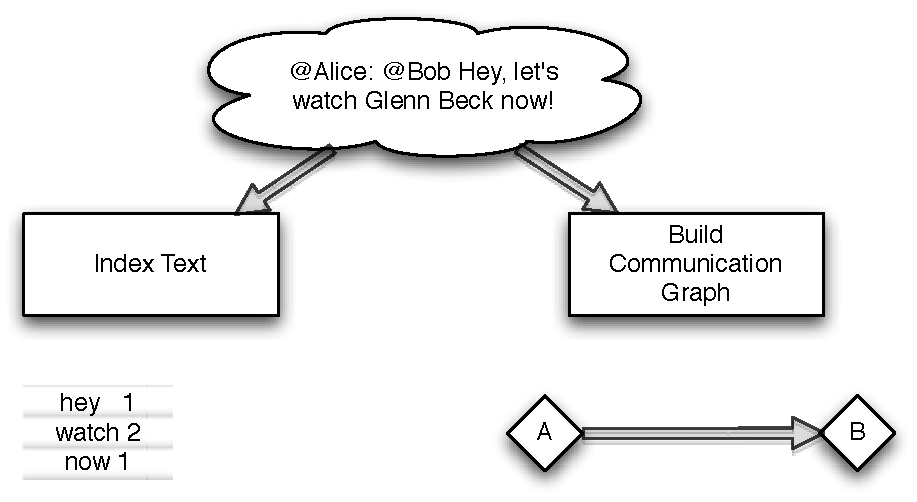
\includegraphics{figures/spie-preprocessing}
\caption{Preprocessing social network data for exploration.  Message text is indexed in a full text search index, and the communication graph is stored in a fast associative map database.}
\label{figure:spie-preprocessing}
\end{center}
\end{figure}
Once those are built, the community sensing workflow proceeds as
follows:


\begin{enumerate}


\item come up with a set of keywords to occur in the community of
interest




\item a seeding pair of repliers about the topic is found




\item a community of replier triangles is grown from the pair




\item the characteristic phrases are found for the community
discourse




\item the fringe of the community is identified, with the choices of
pairs or topics for further iterations



\end{enumerate}

The exploration workflow is shown in Figure~\ref{figure:spie-workflow}.



\begin{figure}[htp]
\begin{center}
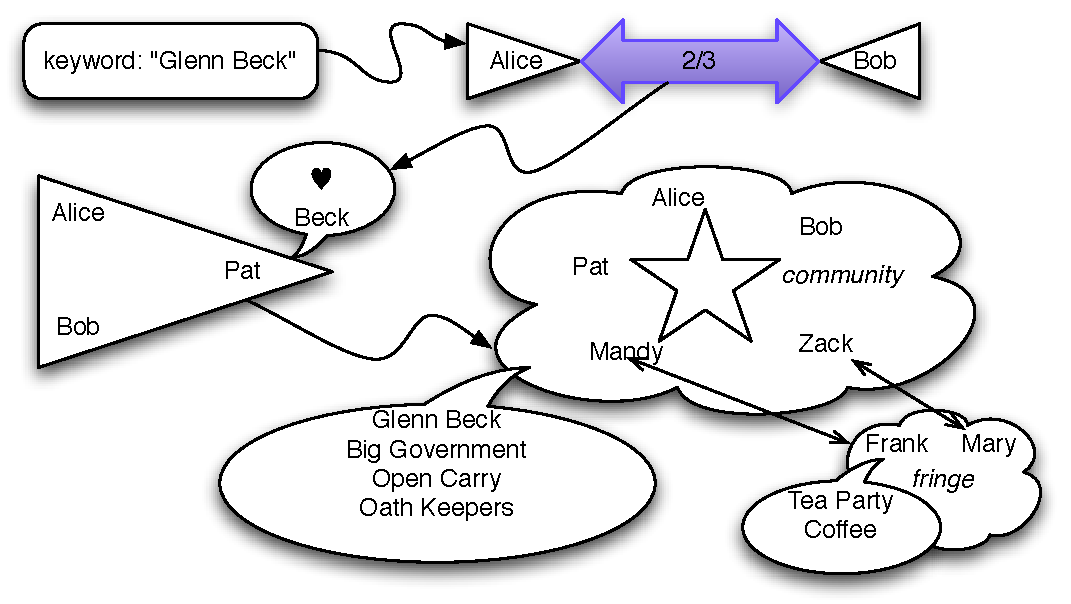
\includegraphics[width=6in]{figures/spie-workflow}
\caption{Exploration workflow.  A keyword is searched and the pairs using it most are found.  Then a community is grown around such a pair, and its topics are extracted.  The fringe and its topics are also listed, allowing for subsequent pivoting and iteration.}
\label{figure:spie-workflow}
\end{center}
\end{figure}
We begin the analysis by searching the Lucene index for pairs of
users who discuss a keyword. All of the twit contents are indexed.
Various twit fields are treated separately, which allows us to find
any replies quickly.


We explored finding both weak and strong pairs of users. A weak
user pair is a pair of users who at least once in their corpora use
the same keyword in at least one of their twits and additionally
have at least one directed message between them. A strong pair of
users has at least one directed message between them which uses the
keyword being searched for. For our analysis we used strong user
pairs finding that they gave us results more like what we were
attempting to find as a community. Additionally, before generating
communities based on these pairs we pruned them based on the number
of times that the keyword was mentioned between the users.


We then used these user pairs as seeds for growing communities. We
use a recursive community definition based on a triangle property,
such that a user is a member of a community if they have been sent
messages by two of the users of the community. If that is the case,
the ``child'' user is added to the community connected to those two
``parent'' users. The child users are added recursively, until there
are no more users to add. Any users which have been sent messages
by exactly one of the members of the community is considered to be
on the ``fringe'' outside of the community, or simply the fringe.


We perform collocation and Statistically Improbable Phrase (SIP)
analysis on these communities to find the resulting topics of
conversation in the communities. These Natural Language Processing
(NLP) approaches are used to identify the most characteristic
phrases describing the community discourse, approximating
``what are they talking about.''


\pagebreak \section{Previous Exploration Work}
\label{previousexplorationwork}

Community identification in graphs with no specific community marking is an active research area. Flake et al. \cite{DBLP:conf/kdd/FlakeLG00} propose a definition of a community as a group with more links inside than outside. It turns out such a definition requires a simultaneous partitioning of the whole graph into communities to work, and the communities cannot overlap. Mishra et al. \cite{DBLP:conf/waw/MishraSST07} overcome this with a notion of $(\alpha,\beta)$ clusters. A subset of vertices forms an $(\alpha,\beta)$-cluster if every vertex in the cluster is adjacent to at least a $\beta$-fraction of the cluster and every vertex outside the cluster is adjacent to at most an $\alpha$-fraction of the cluster. Such clusters can overlap. Backstrom et al. \cite{DBLP:conf/kdd/BackstromHKL06} use self-declaration as criteria for membership: joining a LiveJournal community, which requires explicit joining, or publishing in a conference for DBLP-based communities. Statistically Improbable Phrases (SIPs) are effectively used on Amazon to characterize contents of books, and they give a very good idea of what a book is about. Savell and Cybenko \cite{Savell:2008:Intelligence} provide quantitative formalisms for social behavior in a group context. Khrabrov and Cybenko \cite{Khrabrov:2010:Dynamic} provide metrics of group cohesion and influence. Sociologists have many useful metrics for community formation, with quantitative measures of influence as well -- Bonacich \cite{Bonacich:2001:Coalitions} and Friedkin {Friedkin:Influence} provide metrics which can be applied directly to many Twitter-mining tasks.


\section{Text Indexing}
\label{textindexing}

For topical search, we index the twits and search them with Lucene
\cite{code:lucene}. Lucene is a powerful open-source search engine which
uses flat-file inverted indices to provide fast full-text indexing
and searching. The fundamental unit in Lucene is a document, which
can have any number of fields, each with a number of indexing
parameters.


We created a custom analyzer for Lucene allowing us to preserve the
meaningful special characters that appear in twits. The indexer
tokenizes the text on characters which are neither letters, numbers
or the @ or \# symbols and creates a full-text search index on
those tokens. We also store metadata for each twit, including the
date the twit was posted to the twitter stream, whether the twit
contains a hashtag, is it directed, and, if so, who it was directed
to.


We created two Lucene indices on a month's worth of twits from the
Twitter {\itshape gardenhose} stream, containing a statistically
representative fraction of all twits (which can be as high as a
fourth). The first index was created with each twit as a document.
A second index was then created on each user's corpora as a
document. Using these two indices we created a number of API
functions to perform textual analysis on the Twitter data.


In order to ensure that we would receive meaningful results from
the analysis of the twitter data we created a custom stop word list
generator which would generate a stop-word list based on the whole
corpora of words used in twits, pruning out some entries by hand
that were clearly meaningful. We created a number of functions
which performed textual analysis on the dataset.


\begin{enumerate}


\item {\itshape topChatters} -- gets the users with the most conversation
messages




\item {\itshape twitUserIds} -- gets all the users and twits for a term




\item {\itshape topWordsByTwit} -- gets the top words in the combined corpora
of the list of twits




\item {\itshape topWordsByUser} -- gets the top words in the combined corpora
of the list of users




\item {\itshape userPairTopics} -- gets the top words for pairs of users




\item {\itshape getStopList} -- creates a stop list from the most commonly used
words in the corpora of all twits



\end{enumerate}

In addition to the API functions which interact with the full index
on a per twit basis we created API functions which operate on the
per user corpora index. These functions primarily use queries with
very large numbers of terms to perform~cosine similarity analysis
on the corpora of a single user or a group of users against another
user or group of users. Through this procedure we are able to
compare a candidate to join a group to the corpora of the group as
a whole in order to rank users who are considered to be on the
fringe of a community for inclusion into the community.


\pagebreak \section{Community Detection}
\label{communitydetection}

Many previous and current popularity metrics for Twitter focus on
the followers graph. Indeed, twitterers create a datastream,
similar to RSS news, by subscribing to -- or following -- other
twitterers. However, as pointed out by Finin et al.
\cite{DBLP:conf/kdd/JavaSFT07}, the number of followers doesn't
necessarily predict influence or social bonds. What matters are
actions -- and in case of Twitter, direct communications, called
replies.


Anybody can address anybody else publicly, by simply inserting the
addressee's nickname, preceded with @, into the twit (then called
reply). We can extract replies from all twits and build a
communication graph out of them. Such a graph can be static, being
a snapshot at a certain time, or dynamic, where nodes and edges are
added with timestamps, constituting a multigraph. When looking for
communities, we propose to do so through the communication graph,
revealing those engaged with each other, presumably over a set of
topics.


Our exploration workflow, outlined in Figure~\ref{figure:spie-workflow},
begins with a search phrase, such as ``Glenn Beck.'' We then identify
pairs of repliers from the communication multigraph who exchange
this phrase in both directions, and sort the pairs by the number of
total exchanges they had. The top pair would be the most active,
and becomes our seed candidate for the community. We grow the
community from that seed pair as follows.


Our community identification algorithms is indirectly inspired by
Backstrom and Kleinberg \cite{DBLP:conf/kdd/BackstromHKL06}, who made
the following observation when studying the dynamics of the
community growth. A new member is much likelier to join a community
when he has two friends already in the community, not yet connected
themselves (an open triad). We simplify it by not insisting the two
friends have no links, but requiring that a prospective member has
at least two friends already in the community.


Hence, the algorithm proceeds as follows. We start (*) with a
pair, $(A,B)$, in a queue, who are the seed members of the
community. They may or may not have a link -- e.g., in one version,
we actually find such pairs which exchanged messages with a topic,
such as ``Glenn Beck,'' in them, while in another, we seed with two
unconnected users, independently interested in the topic. (An
option may further control whether there should be messages in each
direction, signifying mutual interest, i.e.\ at least two, or one
will suffice.) After that, we sort friends of $A$ in the decreasing
order of the total number of messages exchanged, do the same with
$B$'s friends, and then find the first shared friend in the list,
$C$. $C$ is then added to the community, and the pairs
$(A,C), (B,C)$ are added to the queue. The process (*) is then
repeated until the queue is exhausted.


There are certain asymmetries in the communities grown by the
versions of this algorithm where only one direction of the edges
are required. If we allow for a single directed edge as a (topical)
relationship marker, we will get different communities when
starting with the pair $(A,B)$ rather than $(B,A)$. Such
differences can be considered as a result of the bias towards $A$
or $B$, or compensated for by requiring edges in both directions.
Here we ensure symmetry by requiring both edges.


In our studies with several seeding topics, the communities
saturate fairly quickly, conforming to the idea of a tightly knit
cluster \cite{DBLP:conf/waw/MishraSST07} being characteristic for a
community. Figure~\ref{figure:spie-workflow} contains an example where the
seeding pair, Alice and Bob, both talk to a third user, Pat, the
most, hence bringing her into the community. The process is
repeated until no new triangles exist, or until a set limit is
reached. Two kinds of limits can be set: by the total size of the
community, or the distance, in generations, from the seeding pair.
The generations are natural layers, and computed as follows. The
seeding pair members both are generation 0. In a triangle, the new
member gets the lowest parent generation plus 1. The process can be
stopped when a given layer is reached.


The fringe of a community is a set of users connected, in the
communication graph, to at least one member of the community, but
which themselves are not its members. Once the fringe is detected,
its twit set can be examined for SIPs. Those can provide a set of
choices for further exploration, to restart the community building
process. We outline such a process as a basis of data exploration
below.


Community graphs are build from a set of directed edges --
$E(from,to,weight)$ -- where weight is the number of messages which
traversed that edge in the dataset. Since the time sample was so
long, there is an not insignificant number of edges with low
weights. Such low weighted edges represent transient communications
between users and more closely resemble noise than structural
components of the communities.


In order then to create meaningful community structures, the edge
set $E$ must be trimmed of edges with low weight which can, if
further analysis is performed, obscure the tightly knit central
clusters we hope to find. For the data sets used for this paper, we
chose a cutoff weight based on the obvious threshold in the
histogram of the weights on the graph, usually a number of twits
between 1 and 5.


\pagebreak \section{Exploration Results}
\label{explorationresults}

Using the aforementioned analysis procedure we found resulting communities and their related collocations and SIPs for a number of search terms.  We describe one such complete workflow for a political community centered around Glenn Beck.


Glenn Beck is a controversial conservative cable television show host on the Fox News network.  We performed a strong pair search for users who used both ``Glenn'' and ``Beck'' in at least one directed twit.  We then grew communities from the set of the 38 seed pairs that resulted, using the recursive community growth algorithm described above.  We expected that because of Glenn Beck's controversial nature we would be able to find distinct communities with little or no cross interaction.



\begin{figure}
\begin{center}

\includegraphics[width=6in]{figures/gb5}
\caption{The full graph for one of the five major communities found for the the Glenn Beck search.  The node labels are the users unique Twitter IDs.}
\label{figure:gb-full}
\end{center}
\end{figure}

\begin{figure}
\begin{center}
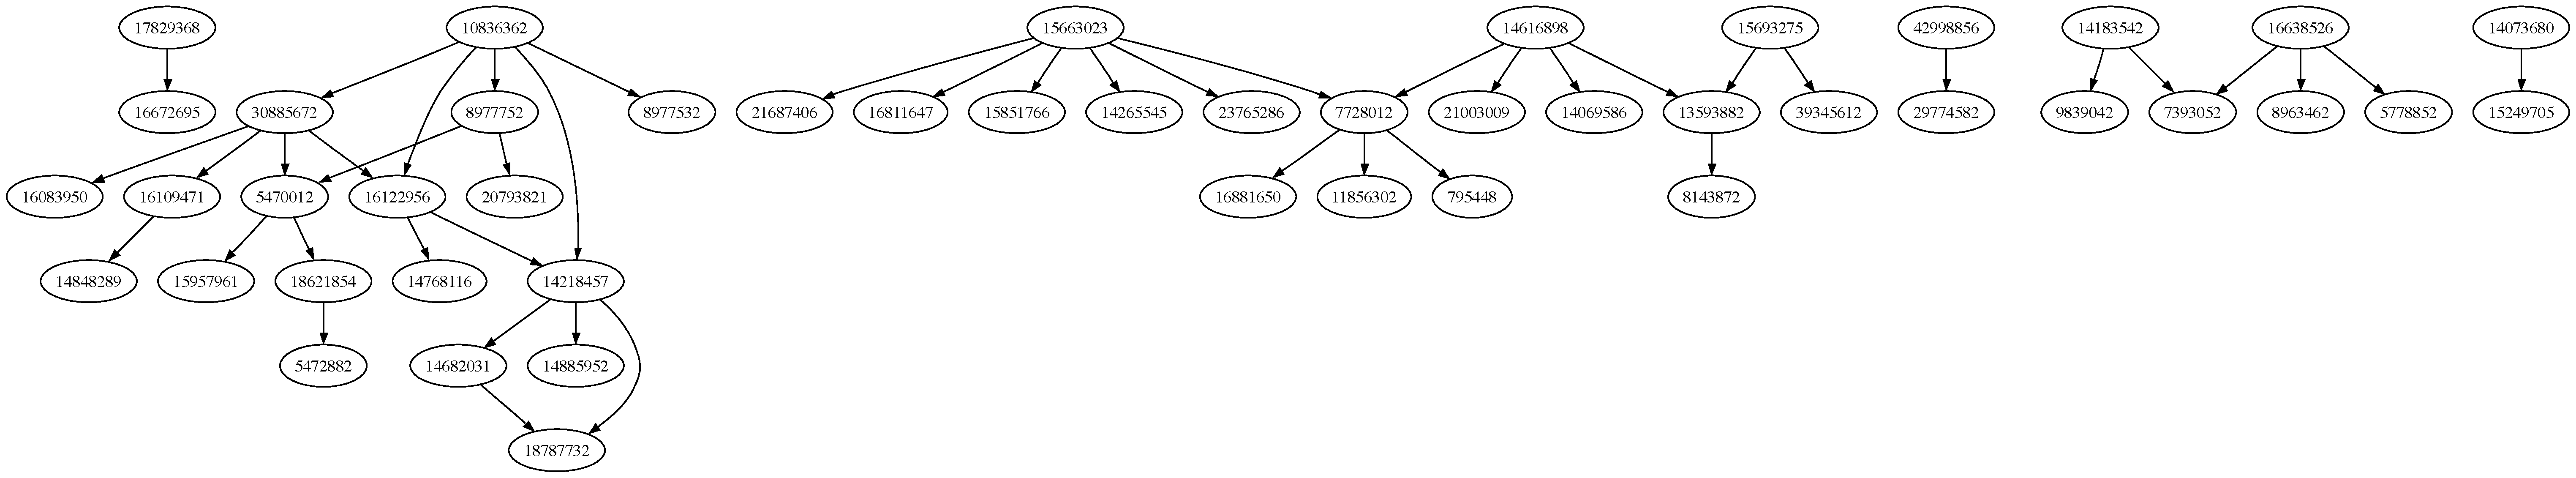
\includegraphics[width=6in]{figures/gb5-reduced}
\caption{The reduced graph for one of the five major communities found for the the Glenn Beck search.  Edges which did not meet a minimum weight were pruned from the graph.  If a node was unconnected after pruning it does not appear in the graph.  The node labels are the users unique Twitter IDs.}
\label{figure:gb-reduced}
\end{center}
\end{figure}
The full graph of the 5 interacting communities can be found in Figure~\ref{figure:gb-full}, Appendix A, ``Full Glenn Beck Graph.''


\pagebreak \section{Discussion Topics}
\label{discussiontopics}

For the communities we identify, we look at the typical topics discussed. One way to find the topics is to look at the top {\itshape n-grams} \cite{Ngram:Chen-Goodman} used in the text of the messages exchanged. These will often be trivial and shared across many communities, e.g.\ bigrams such as ``I need{\ldots}'' A more interesting source for characteristic topics are the Statistically Improbable Phrases, or SIPs. They are widely used on Amazon.com to characterize a book. The SIPs are found by looking at n-grams and comparing their actual frequency to the case where the words would happen to be together randomly. Those n-grams where such repeated co-occurrence is very unlikely for random words are ``improbable'' in terms of randomness, i.e.\ they are uncovering some regularity.


Some of the Glenn Beck community SIPs are shown in Table~\ref{table:gb-sips}.



\begin{table}
\label{table:gb-sips}
    \centering
\begin{tabular}{|c|c|}
    \hline
    Reining Medical Suits & Freedoms First Rally \\
    \hline
    Voting Rights Act & Martin Luther King \\
    \hline
    Gitmo Detainee Lawyer & Convo Gitmo Detainee \\
    \hline
    Able Bodied One & Payer Health Care \\
    \hline
    Speaking Your Truth & Town Hall Friday \\
    \hline
    Henry Louis Gates & Gov Mark Sanford \\
    \hline 
\end{tabular}
\caption{Statistically Improbable Phrases from the Glenn Beck community.  The phrases are trigrams which co-occur much more than random three words would.  They are the political issues and personalities of the day, circa Summer of 2009.}
\end{table}
Our method is a convenient way to browse through a social network.
The Twitter data stream receives millions of messages from millions
of users daily. It's hard to even begin to explore such a
collection. Given the topical community search, we have both an
entry point and a pivoting procedure. After a community is seeded,
grown, and its topics are revealed via SIPs, the explorer can
either stop there and look at the users of interest, or detect the
fringe and pick a topic from its SIPs or a pair with one member in
the community at hand and another a fringe member. That pair, or a
fringe SIP can be used to seed a new community for the next step of
browsing, which we call pivoting.


When keywords contain spatially or temporally localized topics, our
workflow can be used for community sensing -- following the
communities in a specific environment in the topical or
geographical space. For instance, the 2009 crisis in the New York
State Senate can be tracked down using the name of a key Democratic
senator, Pedro Espada Jr., who sided with the Republicans for a
while, only to come back having extracted certain concessions -- and
bringing the senate business to a halt in the mean time, causing
much Twitter debate. Those users who mention his name are likely to
follow the state politics; similar topics exist for engaging issues
in every locale.


\pagebreak \chapter{Influence}
\label{influence}

\label{chapter:influence}


The web becomes more and more interactive and real-time every day.  The original static Mosaic pages were replaced by database-driven merchants and blogs.  An early pioneer of web-based conversation, LiveJournal, appeared in 1999 and still has a majority mindshare in countries like Russia and such communities as programmers and journalists, due to the ease of dialogue.  Comments became {\itshape de rigeur} for  blogs, and now new social media such as Twitter and Facebook are essentially comment and status update-driven.  Comments and status updates are inherently two-way communications, and these social networks may supplant SMS and email, becoming full-fledged communication networks.  Traditional communication networks, such as email, still dominate, and in many cases require analysis, such as has been done on the Enron data set.  When presented with such a dataset, an important question is, who's important here and who's not?  Whose influence should we discern behind the dynamics of the network to understand its processes?


While forming a social circle on Twitter, people often follow those who are authorities on their professional or personal interests.  Since most of the experts now publish their Twitter {\itshape @nickname} on the Web, it is easy to follow them.  In many cases, people ask questions on Twitter as they used to do on blogs, as on LiveJournal, asking for advice on products to buy, technologies to use, travel destinations, restaurants, etc.  Advice is often sought in conversations, and decision are arrived at via consulting the subject or social authorities.  An influential microblogger can make or break a company's reputation, speed up technology uptake, and accelerate a trend or do the opposite.  Thus it's important for those in the public arena to understand who wields influence in the social networks, how they get there, and how this influence evolves over time.


In this paper, we study conversational dynamics influence in communication network graphs.  We use Twitter as a publicly available communication network.  We look at the communication graph formed by messages, or tweets, from one person mentioning another, those replies (or mentions) mapping to an edge in the graph.  We then look at several graph metrics dynamically, computing them for every day in the study, and then look at the users whose metrics dominate, or accelerate faster, or grow longer than others'.  It turns out that such users form interesting classes, and one of our metrics, the {\itshape starrank}, can show when a user becomes a public persona.


We believe that this work can be used in a variety of ways:  individuals can track changes and dynamics of their influence as well as their peers' influence; competitive intelligence analysts can analyze the dynamics of consumer opinions about their products and services with a deeper understanding about who has key influence about attitudes and opinions; intelligence analysis of an organization's evolution and changing roles within an organization.


Java, Finin, et al., \cite{DBLP:conf/kdd/JavaSFT07} look at the power users of Twitter and find that they are indeed superheroes, their energy activated by more replies.  They emphasize the difference between the declared network of followers and the actual network of social interactions. Backstrom and Kleinberg \cite{DBLP:conf/kdd/BackstromHKL06} studied community growth in two social networks, LiveJournal and DBLP (computer conferences).  They looked at a few temporal snapshots, learned some rules of community growth in between, and found some of the graph structures which make such processes as joining a community more likely.  Khrabrov and Cybenko \cite{DBLP:conf/cse/KhrabrovC09} apply sequence modeling to the cell phone tracks of a group of MIT students, using n-gram models and suffix trees.  Savell \cite{Savell:2008:Intelligence} and Chung \cite{Chung:2006:Tracking} have developed techniques for identifying and analyzing business process dynamics within social networks using a variety of methods including Process Query Systems \cite{PQS:2007}.


\pagebreak \section{Dataset and Methodology}
\label{datasetandmethodology}

We started monitoring Twitter using its new Streaming API from June 2009 onward.  Our subscription level, the so-called ``gardenhose,'' provides a fraction of all tweets, which is quite significant: about 2-3 million tweets a day initially, now reaching 4-5 million tweets daily.  The working set for the studies in this paper consists of a 100 million tweets from October 16 to November 17, 2009.   From those, we compute our metrics on the leading 90 million tweets, spanning three complete weeks (22 days to disregard time zone effects).


The replier graph is built from this working set in an incremental way.  For each new day, we add that day's mentions as directed edges, and count them for the source (in number of repliers), and the target (in the number of mentions).  We compute the pagerank \cite{DBLP:journals/cn/BrinP98} of each user at the end of the day, using the Jung2 toolkit \cite{code:jung} with $\alpha=0.15$, over 100 iterations. Given the pagerank for each user, for each day, we define the {\itshape drank} of every user that day as follows:


\begin{itemize}


\item Sort the {\itshape (user,pagerank)} pairs by increasing pagerank;

\item Replace each user's pagerank by its position (starting from 0);

\item Optionally normalize into 0-1 range by dividing by the list's length.
\end{itemize}

Table~\ref{table:drank} contains a step-by-step example of the {\itshape drank} computation.



\begin{table}
    \caption{\emph{Drank} Computation}
    \label{table:drank}

    \centering

    \begin{tabular}{|c|p{2in}|}
    \hline
        [a:0.1 b:0.02 c:0.3 d:0.2] & original user:pageranks\\
    \hline
        [b:0.02 a:0.1 d:0.2 c:0.3] & sorted by pageranks ascending\\
    \hline
        [b:0 a:1 d:2 c:3] & pageranks replaced by position, 0-based - this is the \emph{dirank} \\
    \hline
        [b:0 a:1/4 d:2/4 c:3/4] & normalized by the list length - this is the \emph{drrank} \\
    \hline
    \end{tabular}
\end{table}
The number of users with a given pagerank increases daily, as more and more users get on Twitter and engage in conversation.  The daily number of ranked users is shown in Figure~\ref{figure:daily-users}.



% daily-users
%(396594,789937,1065252,1358559,1591226,1765756,1936809,2097928,2222221,2341354,2478528,2629111,2767989,2892705,3003975,3087760,3176088,3275556,3380727,3487572,3589058,3681171)

\begin{figure}
\begin{center}
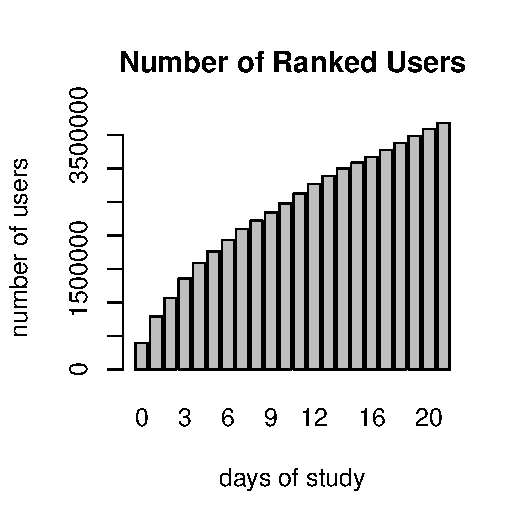
\includegraphics{figures/daily-users}
\caption{Twitter's user base continues to grow significantly}
\label{figure:daily-users}
\end{center}
\end{figure}
Normalization compensates for the ever growing number of users active on Twitter every day.  However, the effects where such growth is interesting are better observed on the integral {\itshape dranks}.  We refer to the integral, non-normalized {\itshape drank} as {\itshape dirank}, and the rational, normalized one as {\itshape drrank}.
Simple metrics such as the number of mentions a user gave or received each day are integers, which, in the dynamic contexts, become integer lists.  We look at the number of repliers (different targets mentioned by the same source), mentions (different replies with the same target), and total number of tweets by a user, daily, which translate into integer lists.


Those histograms contain only those users whose complete corpus is nondecreasing or increasing; a single daily drop will filter them out.  To look at all users, we partition their lists into longest contiguous nondecreasing or increasing subsequences, and compute the maximal length and/or acceleration of such a subsequence.  The acceleration is a ratio of the last element over the first; since many first elements are 1, we also look at a ``tougher'' version, where the acceleration is with respect to the second element; the minimal length of the subsequence in each case is 3, showing at least two days of growth (or no decrease).


Many features related to influence increase or decline along with time, and are represented as a real-valued time series.  Examples are the number of mentions a user receives daily, his {\itshape drrank}, and {\itshape drstarrank}.  Totals such as number of mentions given or received can be counted separately for each day or cumulatively from the beginning of the study.  Below we describe several primitives which we combine for our analyses.


\begin{itemize}


\item {\itshape Contiguous Longest Increasing (generally Monotonic) Subsequences} -- This operation ({\itshape clis}) takes a sequence, an ordering function -- one of $<,\leq,\geq,>$ and partitions it into subsequences such that each subsequence is ordered according to the predicate.  Acceleration for each subsequence is the ratio of the last element to the first; the {\itshape :tough} variant divides by the second instead, skipping the frequent 1 for temporal count sequences.  We can drop the leading 0s also when computing accelerations, or filter for them by multiplying the ratios out against a threashold.  We denote the maximum length of a {\itshape clis} subsequence as {\itshape maxlen}, and the maximum acceleration as {\itshape maxxel} (or {\itshape maxxel-tough}).  Table~\ref{table:clis} gives an example of the {\itshape clis} transform.
\end{itemize}


\begin{table}
    \caption{Cont. Longest Increasing Subsequences}
    \label{table:clis}

    \centering

    \begin{tabular}{|c|p{2in}|}
    \hline
        [1 2 3 0 4 5 8] & original sequence\\
    \hline
        [[1 2 3][0][4 5 8]] & subseqs partitioned by $<$,\emph{maxlen} $3$  \\
    \hline
        $[\frac{3}{1}$ 0 $\frac{8}{4}]$ & subseq accelerations, \emph{maxxel} $3/1$, \emph{maxxel-tough} $8/5$ \\
    \hline
    \end{tabular}
\end{table}
\begin{itemize}


\item {\itshape Grow or Fall} -- This operation ({\itshape growfall}) takes a sequence and counts how many successors are greater or less than their predecessors.  Then a decision is made whether the sequence is mostly ``grow'' or ``fall'' by either the simple ($1:1$) or qualified majority ($2:1$).  Optional {\itshape twice-higher} filter keeps only those sequences where the change between the first and last element is twice or more.  The result can be either categorical -- {\itshape :grow}, {\itshape :fall}, or {\itshape :neutral}; or quantitative -- the rate of change, with 0 for neutrals, and the sequence returned ordered by the rate of change.  Table~\ref{table:growfall} shows an example of the {\itshape growfall} transform.
\end{itemize}


\begin{table}
    \caption{Grow or Fall}
    \label{table:growfall}

    \centering

    \begin{tabular}{|c|p{2in}|}
    \hline
        [1 2 3 5 0 7 6] & original sequence\\
    \hline
         5 pairs up, 2 pairs down & :grow both simple and qualified \\
    \hline
        rate of change is $6/1$ & passes :twice-higher filter \\
    \hline
    \end{tabular}
\end{table}
The {\itshape starrank} considers a user's importance with respect to his neighborhood.  Figure~\ref{figure:starrank} shows a user with his mentioners on a particular day, along with his and their {\itshape drank}s.  The {\itshape starrank} is an average of the neighbors' ranks, weighted by the number of communications with each neighbor for that day.  Depending on the kind of the d-rank we use, we'll get a corresponding {\itshape starrank}.  For instance, a user's {\itshape distarrank} for a day will be an average of the {\itshape dirank}s of her neighbors, i.e.\ of their positions in that day's sorted order of page ranks.



\begin{figure}
\begin{center}
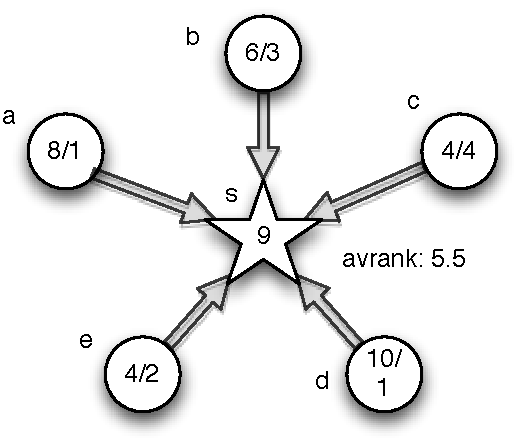
\includegraphics{figures/starrank}  
\caption{Example of \emph{starrank} computation.  The center user with \emph{drank} of 9 is mentioned by 5 other users with the given \emph{drank}, exchanging one or more tweets that day, e.g. $r/n=6/3$ means 3 mentions by a user of \emph{drank} 6.  Then the \emph{distarrank} is the average of $r$s weighted by the $n$s, here $(8*1+6*3+4*4+10*1+4*2)/(1+3+4+1+2)=5.5$}
\label{figure:starrank}
\end{center}
\end{figure}
\pagebreak \section{Influence Findings}
\label{influencefindings}

\label{section:influence-findings}


For individual ranks sequences we can look at the longest growth or decline periods.  We partition each sequence into contiguous increasing or decreasing subsequences and take the longest one.  For the number of mentions, we look at the total amount of users for whom it is nondecreasing, and look at their longest runs over days.  


Figure~\ref{figure:nnm-hist} shows how many users with all non-decreasing mention runs have full seqauences of at least a given number of days.  Each bucket is the total number of users who achieve that many days of stability or growth.



%NNM-HIST starts at 3 days
%c(333355,160407,77648,36657,16797,7293,2985,1145,438,133,40,7,2,1,0,0,0,0,0)

\begin{figure}
\begin{center}
    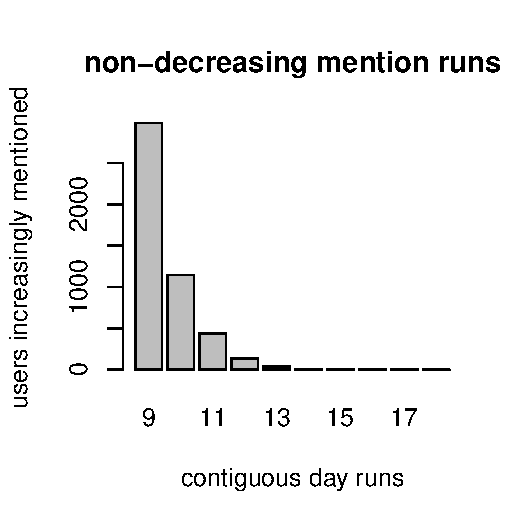
\includegraphics{figures/nnm-hist}
    \caption{The number of users whose daily mentions are all nondecreasing, per day}
    \label{figure:nnm-hist}
\end{center}
\end{figure}
Figure~\ref{figure:irr-hist} shows the same for non-increasing {\itshape dirank}.  The one person who persists to the end is Justin Bieber with the top nondecreasing rank of 0 (see below on the Bieber ``Ecosystem'').



%IRR-HIST
%c(2985,1024,393,159,86,53,31,16,9,6,3,1,1,1,1,1,1,1,1)

\begin{figure}
\begin{center}
    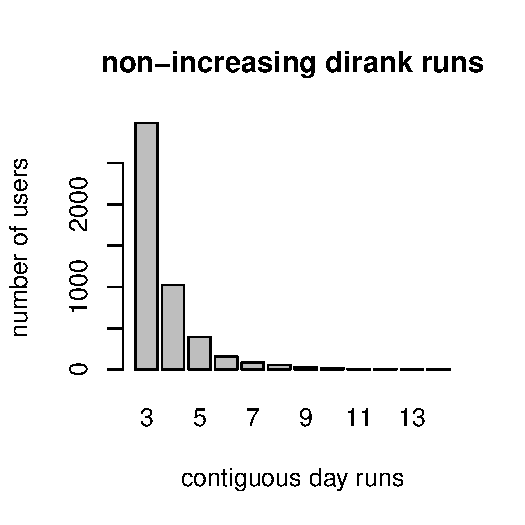
\includegraphics{figures/irr-hist}
    \caption{The number of users whose own daily \emph{diranks} are all nondecreasing, per day}
    \label{figure:irr-hist}
\end{center}
\end{figure}
The users with the longest period of growth in their {\itshape drrank} include the following:


\begin{itemize}


\item Brazilians.  Most of our influence growth metrics for repliers bring up a lot of Brazilian journalists, stars, and power users.  Apparently, Brazilian twitterers are more communicative than others, using Twitter more like a conversation medium than a diary.  The top ones include {\itshape @leobarcellos}, a web designer, {\itshape @natyperdomo}, ``Publicitária,'' and more.

\item {\itshape @alfiehitchcock} -- a London photographer posting his pictures via TwitPic

\item {\itshape @Theresamcardle} -- an ``Optimist; Toilet seat marketer at Kohler; UW-Madison MBA student''
\end{itemize}

Those with the longest contiguous increase in real {\itshape starrank} of mentioners -- i.e.\ losing influence -- include such accounts as \emph{@gm\_web}, an automatic repost of a weather station, and {\itshape @AlexanderFog} -- a self-referential DJ referring to himself in every tweet.


The second-order characteristic of growth is acceleration.  Here, for each contiguous increasing or decreasing subsequence, the acceleration is given by the ratio of the final state to the original value.  For a quantity such as the real rank, where growth means decrease, we invert it, so that the bigger acceleration, the better the growth is.  Once again, the pack of {\itshape starrank} acceleration-sorted users is dominated by many of the same Brazilians, showing that the longest active growth also often is the fastest one.  Some of the new faces here are


\begin{itemize}


\item \emph{@jc\_schuster} -- a country music fan

\item \emph{@drosa\_shannon} -- ``twin,married, love DOOL,BL,American Idol and Tweeting''

\item {\itshape @carlaciccarelli} -- ``Publicit'{a}ria e Produtora de Comerciais,V'{i}deos e Eventos''

\item {\itshape @Dollbabyv} -- a girl writing about her dating, referencing a Blogspot blog
\end{itemize}

The {\itshape starrank} clearly demonstrates how a star constantly spreads its influence through to ever increasing realms of new users, with lower {\itshape dirank}, thus its average audience rank is increasing.  


Figure~\ref{figure:bieber-distarrank} shows the daily {\itshape distarrank} of Justin Bieber, the most influential replier.  It's not normalized to show the effect of the influx of the new users.



%BIEBER-DI-STAR-RANK
%c(263266, 491511,655086,808762,934326,1025713,1062641,1138209,1191615,1258979,1359705,1387844,1452082,1594333,1623814,1452615,1703495,1626026,1688772,1857144,1754914,1728743)

\begin{figure}
\begin{center}
    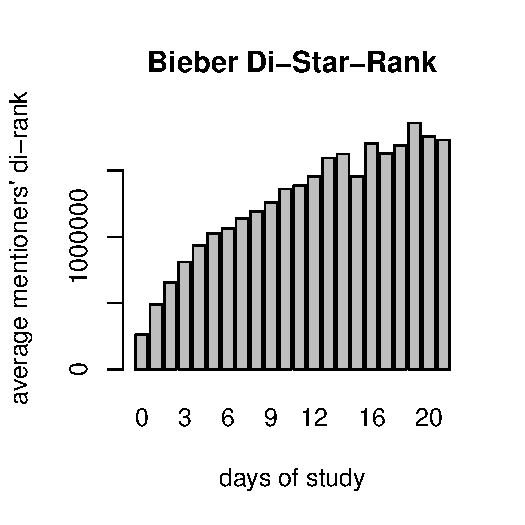
\includegraphics{figures/bieber-distarrank}
    \caption{The average \emph{dirank} of Justin Bieber's fans, decreasing daily, shows his star power spreading to the masses}
    \label{figure:bieber-distarrank}
\end{center}
\end{figure}
The normalized {\itshape starrank}, i.e.\ {\itshape drstarrank}, when decreasing for the longest runs over days, shows the cumulative growth in the importance of a community around the user with respect to all others.  When sorted by such a longest run, we get interesting classes of influential users, such as


\begin{itemize}


\item {\itshape @donniewahlberg} -- leader of the New Kids on the Block band and fans, with far-reaching and active following

\item {\itshape @bowwow614} -- the rapper Bow Wow

\item \emph{@faydra\_deon} -- ``Minister; Computer Applications Trainer; Website Designer; WordPress/Joomla! Customizer; Grammar Queen; Online Bookstore Owner; AKA,'' posting her own ``questions of the day.''
\end{itemize}

Now we look at the acceleration of the {\itshape starrank}, and find the users with the fastest growing communities by importance.  Some of the top users with the accelerating mentioners are:


\begin{itemize}


\item {\itshape @JoycePascowitch} -- ``jornalista, glamourosa{\ldots}.e estressada!'', a Brazilian journalist

\item {\itshape @Biofa} -- ``Jornalista cruzeirense que ama futebol, mulher e rock'n roll (meu Deus, como isso '{e} bom!!!!)'', a Brazilian sports journalist

\item {\itshape @Dejdia} -- apparently a photographer in LA, using a Flickr page as the URL, with her own ecosystem of fans

\item \emph{@Minni\_w} -- ``ddub Soldier (Army of NKOTB)'', a fan of {\itshape @DonnieWahlberg}, one of the top-page-ranked users, the band leader for the New Kids On The Block (NKOTB).  She connects with the Bieber network (see below).
\end{itemize}

The snapshots of the pagerank relationship to number of mentions reveals certain stable patterns.  We cluster the pagerank vs. number of mentions graph into groups of 1000 points, and take the median of $x$s and $y$s to plot, which we call a blocked projection.  Figure~\ref{figure:harp} shows how the resulting graphs form a ``harp'' pattern which stays stable through days 10 and 20.  We filter on $x$ to stay within 25 median mentions on a day, the remaining few clusters group the outliers with exceptional dynamics (or statics).



\begin{figure}
\begin{center}
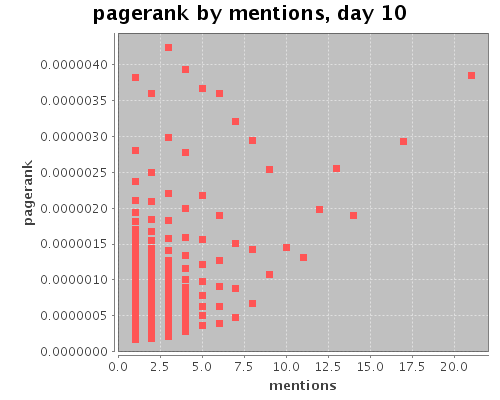
\includegraphics[height=3.5in,width=3.5in]{figures/points-nments-prank-10}
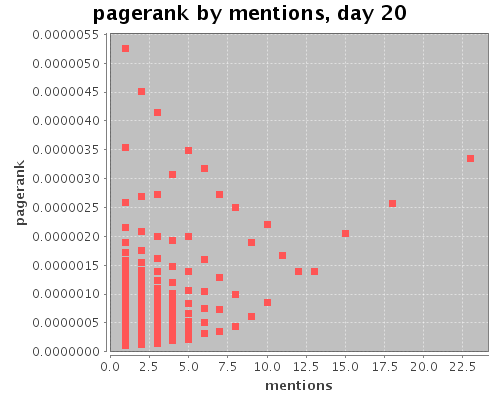
\includegraphics[height=3.5in,width=3.5in]{figures/points-nments-prank-20}
\caption{Pagerank improves with the number of mentions only so much, then ratcheting mentions is counterproductive.  The harp pattern persists \label{figure:harp}
throughout the days}    
\end{center}
\end{figure}
A similar pattern persists for the relationship between the pagerank of a user and the sheer number of twits by that user.  A block projection in Figure~\ref{figure:ctwits-prank} shows that twittering more gets you only so far, and then your ranking starts to fall again.  We show it for day 20, day 10 is similar.



\begin{figure}
\begin{center}
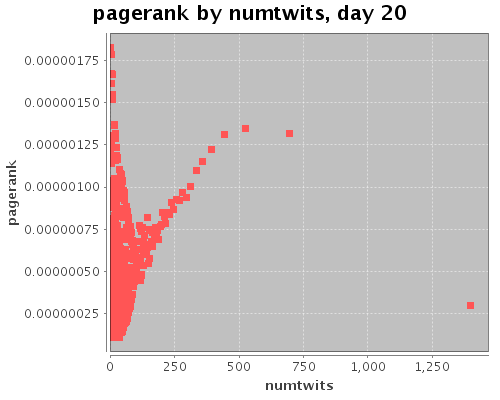
\includegraphics[height=3.5in,width=3.5in]{figures/points-ctwits-prank-20}
\caption{Pagerank improves with the number of twits only so far as well.  X is the cumulative number of twits, Y is the resulting pagerank} 
\label{figure:ctwits-prank}
\end{center}
\end{figure}
\pagebreak \section{The Pagerank Generation}
\label{thepagerankgeneration}

\label{section:pagerank-generation}


The most surprising discovery in the Twitter network we made is the Bieber ecosystem.  Its growth principle can be summarized as: {\itshape You can't be Justin Bieber, but you can be Amanda D}.  The person with pagerank 0, i.e.\ the most influential person in Twitter mentions in our dataset, each day, every day of the study, is Justin Bieber.  Not many people over age 15 know who he is, despite his Christmas 2009 performance at a Washington, D.C. concert for President Obama.  An informal polling of seminar participants and friends over 18 confirms an almost absolute lack of Bieber awareness.  At the same time, Justin Bieber, a YouTube boy singer phenomenon, commands a significant mindshare among the pop culture fans from about 11 to 15 years old, from Brazil to Slovenia, but mostly teen girls in Canada and the US.


The most interesting aspect of the Bieber Ecosphere is that it's the first Twitter generation which grows up with social networks in hand, and adapts to its influence seeking ways almost naturally.  They evolve to efficiently rise in the page ranks.  The second and third daily position by pagerank are most often occupied by several high-caliber fans of Justin Bieber.  One of them, Amanda D., self-billed as a singer and songwriter in the South, is too young to drive, and her parents wouldn't take her to a Justin's concert in the nearest big city, so one of her online goals is to get him to perform in her hometown -- as described on a free blog website with a link offered to Justin and others to share.  What's most fascinating of the self-named ``beliebers'' is their active and incessant manipulation of the pagerank by constantly mentioning each other and growing the followers' network.


Mentioning another fan is called a ``shoutout,'' which are offered for trade on a quid pro quo basis -- ``SHOUTOUTS FOR SHOUTOUTS!''  Multiple accounts are created for special purposes, e.g.\ {\itshape @wewanttomeetjustin} is maintained by the two top {\itshape beliebers}, for the purpose of aggregating other fans who want to meet Justin, discussing venues, options, plans, etc.  User {\itshape @BieberFame} has created a separate {\itshape @JBieberCash} account, noting its creation date and that Justin followed the same day, and openly referring to the original account as the creator.  Very common tweets state that the number of followers is almost near e.g.\ 10,300, with only about 50 remaining, so all new followers will get a follow-back and a shoutout.  Many tweets are simply multiple shoutcasts, i.e.\ lists of names.


The top {\itshape beliebers} got where they are by active and clever Twitter presence, increasing their influence in a variety of ways.  They trade shouts and create multiple Twitter accounts for focused subgroups, tending them regularly, and team with other top {\itshape beliebers} to do it, positioning themselves at the head of the pack.  They also claim to maintain special relationship with Justin, direct-messaging with him, and offer to relay other fans' question via this exclusive channel.  As far as we can see, these advantages are real -- Justin mentioned both two top {\itshape beliebers}, thus propelling their pageranks to the top.  The {\itshape starrank} pattern of the top fans resembles that of the stars themselves, showing a steady increase of mentions and increase of the average rank of the mentioners, propagating ``into the masses.''  Amanda is so popular and effective that she got her own fan account, ``Amanda D's Army,'' in turn run by one of the top-level Bieber fans using the same techniques which proved to work so well with Bieber's fans.


{\itshape @Kekeinaction} shows up high in the list of the longest contiguous growth in {\itshape distarrank} of mentioners, on almost all days of the study (21).  She maintains heavy cooperation with a lot of other Bieber fans, and also was a star of the movie {\itshape ``Akeelah and the Bees.''} This shows how the younger segment of the audience, focused on teenage culture, is densely connected.  Another example is a top fan from Slovenia, \emph{@jbieber\_fever24}, discovered at 7th position of the longest {\itshape distarrank} decreasing runs.  Her bio reads,
``Hey I'm Tea I'm from Slovenia and I'm 14.I LOVE Justin Bieber!I also like Tay Swift,Miley Cyrus and Sel Gomez!Justin followed me 25/10/2009!''  She uses all the tricks in the book -- trading shoutouts, ramping up the number of followers, maintaining multiple accounts such as  \emph{@JBieber\_Babes}, and inviting other fans to participate in all of those activities together.


\pagebreak \chapter{Reciprocal Social Capital}
\label{reciprocalsocialcapital}

\label{chapter:social-capital}


Social networks such as Twitter and Facebook increase their mindshare daily, and many online activities are determined by the interactions there. In order to understand the dynamics of social networks (``what's happening''), we want to identify the key players -- those participants who are in some way important, influential, and possess certain social capital. Although these terms are used in sociology and computer analysis of static networks, we need to come up with the new and more rigorous definitions in the face of the new users getting on Twitter daily, making the network inherently dynamic. Our solution is a set of dynamic metrics of importance, called {\itshape D-Rank} and {\itshape StarRank}, which allow ranking over time and in comparison to one's audience (network neighborhood). Using these metrics, we uncover fascinating worlds inside Twitter, such as the Justin Bieber ecosystem and Brazilian sport journalists with their fans. Building upon the insights from those communities, we define our version of Reciprocal Social Capital as an iterative update rule, rewarding those who facilitate balanced and stable communication. Running a complete world emulation with our rules, we end up with the social capital distribution which places the hard-talking ``middle class'' nodes at the top, leading to a new ranking and understanding of the Twitter dynamics.


\pagebreak \section{Modeling Social Capital Overview}
\label{modelingsocialcapitaloverview}

Given a large social network changing over time such as Twitter, how do we find the key people who are important, influential in some sense, and have certain social capital -- and how do we formally define and measure these terms? Computer and social scientists, economists, operation researchers, and educators have all proposed quantitative and qualitative approaches for describing social capital. As a consequence, the term ``social capital'' is so widely (over)used since the 1980s that some researchers shy away from it altogether \cite{jackson2008social}. Furthermore, the three qualities listed often overlap. We define them usefully and distinctly for our networks, applying these new definitions to find interesting phenomena such as fan-based economies of ratings and trends, and multi-modal collaboration of hackers, advancing open-source projects online via social coding.


The modern economy is knowledge-based, and knowledge generation closely corresponds to value and wealth creation. The processes where knowledge is created, refined, and made actionable, are increasingly shifted into social networks on the Internet, embedded in social media sites such as Twitter and Facebook, or underlying cooperation on Wikipedia, the social coding portal GitHub, etc. Certain members and groups are key to the value-creating processes in these networks, where people are united by the information they work with. Those individuals contributing the most and best knowledge, or processing it in the best way, are recognized as the main contributors, and get to set the agenda for the whole group. In fact, a lot of communications are questions for the senior members, seeking explanation or coordination. It is important to quantify which members gain importance in these mind economies to know how they work.


The quintessential mind economy is the programmers' community. Their industry, spawning startups in the Bay Area, Pacific Northwest and elsewhere, trades in ideas becoming code becoming startups becoming large companies like Amazon and Google. (In turn, the geeks' ethos epitomized by these companies reflects back on the society where they thrive.) The resources traded by hackers are most commonly URLs of code repositories on \href{http://github.com/}{github}\footnote{\href{http://github.com/}{http://github.com/}}, the open-source social coding portal. Github is organized around \texttt{git}, a distributed source code management system (SCM) authored by Linus Torvalds and originally used to develop the Linux kernel. Now it is a {\itshape de facto} platform to collaborate on open-source projects. While github is used to store and modify the code, people working on it often converse on the Internet Relay Chat (IRC) and Twitter. Some of the most active geek communities on Twitter center on advanced programming languages such as {\itshape \#scala}, {\itshape \#clojure}, and {\itshape \#haskell} -- these are the ``hash tags'' used to mark tweets so that they can be found as a group. Coincidentally, these are also the names of the corresponding IRC channels.


Another community with high traffic is what we call Justin Bieber ecosystem, discovered and described in \cite{Khrabrov:2010:Dynamic}. Justin Bieber is a boy pop-singer phenomenon, originating on the YouTube and spawning an intense following there and on Twitter. Many of his fans are teenage girls with a variation of ``bieber'' in their Twitter nick and are united in their adoration of \texttt{@justinbieber} and pushing him up into the top 10 trending topics on Twitter. In this process, the members learn to increase their own ratings by swapping shoutouts (mentions) and trading shoutouts for follows. An economy of rating-increasing behavior develops. Those who get followed by Justin Bieber increase their standing among the ``beliebers'' immensely, as do those who organize other fans around better schemes ``how to meet Justin.'' High-intensity group behaviors are key in social dynamics and change, and can be studied for the first time on a coherent social organism of a Twitter community with its drivers and influencers, and the methods they use to direct it.


\section{Approach}
\label{approach}

In this thesis, we approach the problem of importance via dynamic analysis of the communication graphs. We build a communication graph of mentions, where one user talks to another via public tweets. E.g., if \texttt{@alice} tweets: ``\texttt{@bob}, did you see this: http://bit.ly/xyz'', she {\itshape replies} to \texttt{@bob}, who is thus her {\itshape replier}, while she is his {\itshape mentioner}. While many Twitter analyses and ranking sites focus on the number of followers \cite{DBLP:conf/kdd/JavaSFT07}, we prefer communication as a form of active behavior with its many social implications, manifesting itself similarly in social media networks, email networks, and real life.


Traditional sociology measures betweenness and centrality on static graphs \cite{bonacich1987power}. Their networks are small and their tools are often Excel spreadsheets and add-ons. By contrast, our data subset consists of a 100 million tweets by 5 million users, with both numbers growing over the period of 35 days. (In turn, our subset is selected from the ``gardenhose,'' a Streaming API for a ``statistically representative'' fraction of Twitter, spewing now 5 million tweets daily, from which we collected billions of tweets.) We have to take temporal nature of these data into account as a key feature of the model.


First, we propose a measure of importance we call Dynamic PageRank, or D-Rank \cite{Khrabrov:2010:Dynamic}. For every day in the study, we treat the communication graph as a directed multigraph (as Alice can easily tweet Bob thrice day) and compute the PageRank of all the nodes present that day. We translate such PageRanks into relative ranks, from 0 to 1, showing where the node stands in the overall sorted list of ranks.


We then define StarRank as a ratio of a node's D-Rank to the average D-Rank of its communication partners. There are also variations where we count a node's repliers and his mentioners either together or separately. Both D-Rank and StarRank can be compared across days, even though the number of nodes on Twitter increases every day.


\pagebreak \section{What is Social Capital}
\label{whatissocialcapital}

We propose a mathematically well-defined measure of Social Capital, which we call {\itshape Reciprocal Social Capital}.  It accrues for those dialogue participants who better maintain their question-answering balance in conversations -- they do reply to those who address them, and get replies from those to whom they talked before. This capital can also favor stronger ties, where you keep talking to your current interlocutors, or it can reward exploration of new partners. The model is parameterized with weights (rewards) for different kinds of behaviors, and previous capital decays with time.


Most definitions of Social Capital are in fact just other kinds of importance measures. E.g. Getoor \cite{Licamele:2005:Benefit} simply uses the term to denote the number of your co-authors on conference program committees. A good review of the definitions of social capital used in computer science is provided in \cite{Motidyang:2007:Thesis}. We model our {\itshape Reciprocal Social Capital} on the social capital of Tuscany villagers who remember how many times they had lent everyday items like salt to each other, versus how many times they got even by borrowing some anchovies, or more salt, in return. A good working description of this kind of local social capital is provided in e.g.\ \cite{Gaggio:2007:Gold}. Every community member in those social-capital-rich areas has a clear mental balance of the favors given and received, which figures in every subsequent social and economic transaction.  The communities are cohesive and mutually supportive, which enhances their quality of life dramatically.  Every Briton or American dreaming of moving to Italy refers to that living social capital as a desirable quality in their real social network.  We'd like to model it in the online ones.


Our first computational model is ``reciprocal'' repayment of communications -- instead of a carefully maintained balance of favors, we have a communication network where you repay questions (mentions) by replying (mentioning in return). There's a temporal notion of capital accumulation, along with its decay in the face of inaction.


When looking for influence in social networks, several classes of problems turned out to be closely related to our definition of influence in a community. We addressed them in the additional papers on which this thesis also builds.


In \cite{Khrabrov:2003:Attacks}, we considered the question of network structure which enables the networks to withstand random faults or malicious attacks, taking out some nodes one by one. It is one of the first papers which studied the malicious attacks on a network, and compared behavior of differently structured networks, such as scale-free or random, under different destructuring scenarios. It is an application of dynamic graph analysis, examining how the influential nodes can help keep the network together.


In addition to Twitter, we studied a sensor-based social network, resulting from the MIT Reality experiments \cite{Eagle:2006:Reality}. A fundamental question in dynamic systems is the agents' identity. We address it in \cite{Khrabrov:2009:Language}, where we were able to identify a majority of the MIT Reality participants from just about 10 hops in their cell phone traces. Social importance of the subjects is related to their patterns of action (motion) and resulting interactions.


\pagebreak \section{Reciprocal Social Capital Definition}
\label{reciprocalsocialcapitaldefinition}

Now we will define our metric inductively.


{\itshape Repliers} of a node are the addressees of its tweets. {\itshape Mentioners} of a node are those who tweet to it. If a tweet from \texttt{@alice}{\itshape mentions \texttt{@bob}, then \texttt{@bob} is a replier of \texttt{@alice} and \texttt{@alice} is a mentioner of \texttt{@bob}. To recap, replier of a node is someone that that node repliers \_to}. In other words, from a node's perspective, repliers are out-degree, mentioners are in-degree.  We define the following variables.



\begin{tabular}{|c|p{4in}|}
\hline 
symbol & definition\tabularnewline
\hline
\hline 
$S_{v}^{t}$ & Social Capital of node $v$ at time $t$. Superscript $t$ generally
denotes "by time $t$." Specifically \emph{during} time step
$t$ is denoted as $@t$.\tabularnewline
\hline 
$G^{t}(V,E)$ & graph $G$ with nodes $V$ and edges $E$\tabularnewline
\hline 
$w_{uv}^{@t}$ & total weight of directed edges $u\rightarrow v$, i.e. the number
of tweets from $u$ to $v$ during time step $@t$\tabularnewline
\hline 
$W_{uv}$ & total number of undirected edges between $u$ and $v$: $W_{uv}=w_{uv}+w_{vu}$\tabularnewline
\hline 
$B_{uv}$ & Balance of back and forth tweets from $u$ to $v$: $B_{uv}=w_{uv}-w_{vu}$\tabularnewline
\hline 
$M_{u}$ & $\{v|w_{vu}>0\}$, i.e. the mentioners of $u$\tabularnewline
\hline 
$R_{u}^{@t}$ & $\{v|w_{uv}^{@t}>0\}$, i.e. repliers of $u$ specifically during
the timestep @$t$\tabularnewline
\hline 
$O_{uv}^{@t}$ & outgoing activity of a node rewarded by social capital at timestep
$t$\tabularnewline
\hline 
$A_{uv}^{@t}$ & incoming activity in this cycle rewarded just for mentions (all)\tabularnewline
\hline 
$B_{uv}^{@t}$ & incoming mentions in this cycle repaying previous replies (balance)\tabularnewline
\hline 
$\alpha,\beta,\gamma$ & model parameters\tabularnewline
\hline
\end{tabular}
\begin{eqnarray}
O_{u}^{@t} & = & \frac{1}{\sum_{V^{t-1}}O^{@t-1}}\sum_{v\in M_{u}^{t-1}\cap R_{u}^{@t-1}|B_{uv}^{t-1}<0}|B_{uv}^{t-1}|w_{uv}^{@t-1}W_{uv}^{t-1}S_{v}^{t-1}\\
B_{u}^{@t} & = & \frac{1}{\sum_{V^{t-1}}B^{@t}}\sum_{v\in M_{u}^{@t-1}|B_{uv}^{t-1}>0}B_{uv}^{t-1}w_{vu}^{@t-1}W_{uv}^{t-1}S_{v}^{t-1}\\
A_{u}^{@t} & = & \frac{1}{\sum_{V^{t-1}}B^{@t}}\sum_{v\in M_{u}^{@t-1}}w_{vu}^{@t-1}W_{uv}^{t-1}S_{v}^{t-1}\\
I_{u}^{@t} & = & \gamma B_{u}^{t-1}+(1-\gamma)A_{u}^{t-1}\\
S_{u}^{t} & = & \alpha S_{u}^{t-1}+(1-\alpha)(\beta O_{u}^{t-1}+(1-\beta)(\gamma B_{u}^{t-1}+(1-\gamma)A_{u}^{t-1})
\end{eqnarray}

Some notes on the definitions. $O_{u}^{t}$ is the node $u$'s output gaining social capital, thus we want to reward those who redress an imbalance of input and answer those who addressed you more than you had answered them. The summation is defined exactly over those with whom you have a deficit in replying: $v\in M_{u}^{t-1}\cap R_{u}^{@t-1}|B_{uv}^{t-1}<0$. It means the target node mentioned you at some point prior, you replied to it in this cycle, and before that, you owed it a reply since it tweeted more to you than you did to it. For each such deficit node you replied to, finally, we multiply the number of replies in that cycle, $w_{uv}^{@t-1}$, by the balance you owed, $|B_{uv}^{t-1}|$, the value of the relationship, $W_{uv}^{t-1}$, and the importance of the replier $S_{v}^{t-1}$. We normalize the $O$'s so that they all sum to 1, and reward each node proportionally to the value of the redress in the reply imbalance it actively contributed in this cycle.

Similarly, $I_{u}^{t}$ is the node $u$'s input worth of social capital. We generally consider all input as good — we can't distinguish bad publicity, or consider it all good anyways — but we distinguish mentions redressing the mentioners' own deficit with us as worthing more than just any mention. Those repaying mentions we reward with a multiplier for the balance owed additionally to the usual cycle contribution, relationship value, and the mentioner's social capital.

Note that in the output, we don't have a general activity term for all replies, even those not redressing an imbalance, as we do in the second term of the input. Thus we don't reward random replying, and you won't get social capital by just addressing everybody in volume.

It's easy to see that such a definition of social capital allows for an iterative economy by launching the update rule defining $S_{u}^{t}$ in terms of $S_{u}^{t-1}$ as shown in the last formula above.
The core questions, which may allow for more quantitative treatment with our metrics:


\begin{itemize}


\item Why do people twitter? What is the utility and can it be captured by a form of social capital? Can a single definition suffice for all members of a network? Do ``beliebers'' differ from hackers and how, with respect to their forms of social capital and behaviors increasing it?




\item How can you increase your social capital or importance in the fastest, but most robust (``honest,'' irreversible) way? How can we distinguish fake importance from the real thing?



\end{itemize}

\pagebreak \section{Capital-Based Mining}
\label{capital-basedmining}

Given our metrics of importance and social capital, we explore interesting individuals from our large Twitter data set and interpret what these metrics mean in real life. 


The first results of our full-world Social Capital emulation show a new kind of nodes at the top, in addition to the usual suspects such as Justin Bieber (still in the top 10) -- we call it ``the middle class of social networks.'' These are the people with a certain amount of followers -- though not as many as the stars -- e.g.\ from a 100 to a 1,000, weaving a web of intense dialogues with other such nodes. They provide the core of the ongoing communication, pushing trends and stars up, bringing uninteresting subjects down by not talking about them, integrating other nodes and beginners into the system. We believe our metrics are more interesting than the traditional PageRank in that they reflect the dynamic nature of the conversational networks and highlight the groups making lasting ongoing contributions.


A typical example is beauty industry. Two owners of Singapore beauty salons come on top in terms of continuous conversation threads kept the longest. They discuss wedding photos, haircuts, design, etc. They have a constant and purpose-driven market, thousands of followers each, and discuss news of their industry. This way they keep tabs on their market niche, satisfy their followers with specific goals, and stay on top in the ratings.


Hence one of the differences in the utility of tweeting. Celebrities, those most followed in a typical definition, often get on top by projection from the real world, YouTube, etc. They don't have to tweet for their supper, so to speak. On the contrary, their top fans and other in-Twitter ``phenomenal'' users have to work for it. While spammers achieve a short-term notoriety by mass following, hoping for automatic follow-backs, we do not register those numbers, since we look for real conversations and mentions. Top celebrities like \texttt{@donniewahlberg} and \texttt{@justinbieber} understand this and cultivate their fan base, encouraging top fans once in a while. The timing feature of our metrics smooth over the spikes typical in social networks and reveal true value.


\pagebreak \chapter{Success is Earned}
\label{successisearned}

\label{chapter:success-is-earned}


\section{Accidental Influentials, or Not?}
\label{accidentalinfluentialsornot}

In the 1955 seminal book ``Personal Influence,'' Katz and Lazarsfeld proposed the concept of influentials in social networks, propagating and filtering media streams in their communities.  Although the focus of their study was information diffusion, Katz and Lazarsfeld for the first time fused media studies with dynamics of social groups at local level, and they identified many features of their opinion leaders which position those influentials as important community members by many criteria.


Watts and Dodds, in their 2007 paper ``Influentials, networks, and public opinion formation'' \cite{watts2007influentials}, popularly known as ``Accidental Influentials'' \cite{hbr2007list}, had shown that for a diffusion model with cascades, it's not necessary to have influentials to excite a typical network -- it's mostly the average low threshold on excitability of a majority which decides whether a full cascade will occur or not, instead of who started it, an influential or not.  Despite the specific setting, Watts and Dodds's idea that influentials are somehow ``accidental'' took a life of its own, and was reported by Harvard Business Review as a number one idea on list of the influential ideas for the year (presumably not accidental).


Since we study influence in real social networks, we took this question as a starting point, and for our family of metrics, ask: are our influentials accidental, or not?  And what can this question possibly mean, for a broad class of definitions of influence, which are many?


Let's say that we pick some definition of influence which suits a problem at hand.  The only general requirement for an influence measure we impose is that it establishes an order, or ranking, among all of the people in the study; and that the ``top influentials'' are simply the most highly ranked people in this list.  A consideration of influence then can focus on the very top, or look broadly at the classes of influence, similarly to the rich, the poor, and the middle class in a human economy.


Then our question can be made more concrete as follows: if influence is a function of behavior and connectivity, can we generally say that somebody becomes influential due to their ``intrinsic'' qualities, such as efficient behavior, or, on the contrary, is their influence mostly a product of luck, such as the propitious time and place of that individual's appearance in the network?


\section{Taught by Randomness}
\label{taughtbyrandomness}

The way to answer a philosophical question about whether something is random in this world or not is to create parallel worlds with slightly different rules, mix them with the real one at some point, and see what happens in the same way --- or differently.  When creating the new worlds by varying one feature at a time, we can hope to tease apart the features which make a difference in the course of events.  In this world, there's only one Twitter, albeit its character is constantly changing.  For any given dataset, we have only one order of influentials for any one metric.  However, we can separate the components of behavior which contribute to that influence, and, preserving some part of the network position and some of the behavior, alter the other parts, to see how the influence is affected.  By teasing the starting conditions and the behaviors apart, we can hope to get to the root of our main question.


We introduce a series of strategies to grow the graph from some point onwards, using a combination of behaviors which we reward in the actual graph, as the rewards in the random ones.  First of all, we keep the dynamic characteristics of all simulations the same in the following sense:


\begin{itemize}


\item we add the same new users on the same days as in the original graph

\item every user has the same outdegree for each day as in the original graph
\end{itemize}

Thus, we only rearrange the sinks of some edges in the simulation, after a certain point in time.  We use three classes of strategies to attach the edges:


\begin{itemize}


\item local utility -- optimizing exactly the same reward used to compute the social capital used to rank influence in the first place, but only for the action under control of a node, i.e.\ to whom it will reply (not from whom it will get the replies).  The latter would be a global optimization, while the former is still an individual one.

\item local friends-of-friends -- this strategy attaches to a friend of a friend with attractive characteristics, e.g.\ likely to be seen due to a large number of his/her own friends, mentions, or their own reciprocal social capital.

\item global -- this strategy approximates following users notable via global phenomena, such as celebrities or trendy ones, or efficient communicators with overall leading social capital rank.
\end{itemize}

In each simulated world, we mix these strategies via jump probabilities, creating a composite behavior, hopefully capturing some subset of the real world.  We see who wins in the simulated world, and compare the winners in each position, or rather class, to the real ones for that day and class.  We seed the simulated world with the real one, hence establishing communication balances, friends-of-friends networks, and social capital distributions in advance, in different proportions.  If starting conditions are key, and simulation strategies are reasonable, we'd see the original winners keep their place in large numbers.  By varying the degree of randomness in the simulated strategies, we can see how quickly the winners dissipate from either the real or the simulated world.  If the simulated world is governed by it own rules which are self-consistent, we'd see the same winners across days, even though different world might have different sets of winners; when, once emerging, the winners will persist for the duration of the world, it will mean their behavior is consistent with the rules of that world.


Additionally, we can alter only a specified subset of users, such as those in a given set of buckets.  Using this fine-grained filter on top of a given strategy, we can see which classes fit the strategy better, and if they don't, does it make a difference.


The remainder of this chapter is structured as follows.


\begin{itemize}


\item Reciprocal Social Capital -- we introduce our definition of social capital and the iterative algorithm to compute it on a dynamic communications graph.

\item Methodology of Influence Studies -- the fundamentals of our parallel world simulations and extracting regularity through overlaps with reality

\item Simulation Strategies -- how the parallel worlds are constructed

\item Actual Simulations -- the simulations we ran, composed of the strategies above

\item Simulation Tables -- a cross-linked hierarchy of three levels of tables with key results
\end{itemize}

\pagebreak \section{Methodology of Influence Studies}
\label{methodologyofinfluencestudies}

We use our reciprocal conversational social capital as the measure of influence.  We define and compute it iteratively for each day.  Once the capital is computed for each user in a time period,  we can rank all users according to their social capital for that period (daily).  The top-ranked users are the most influential in this metric.


A fundamental feature of our study similar to Katz-Lazarsfeld and different from Watts-Dodds is the reliance on conversations as pathways of influence.  In fact, this tradition in sociology originates at least with Tarde, who called attention to  the \emph{statistique de conversation} (Tarde 1898) \cite{tarde1969communication} as a means of quantitative study of public opinion.


What does it actually mean to have influence according to the reciprocal social capital metrics?  One gets to the top in this metric by being attentive to one's balance of communication, and by maintaining a high absolute value of dialogues with other partners who also have high social capital, i.e.\ by being an effective communicator and maintaining a good standing in a community of other effective communicators.


The form of influence we consider directly relates to the communication pathways.  Our influencers carry the bulk of actual conversations, which is shown in the volume metrics.  Diffusion models, such as Watts-Dodds, define influence as an ability to propagate information through the social graph, specifically igniting cascades which will affect a bulk of the network.  We submit that prior to any such diffusion begins, the channels of communications must be established, such as conversational links, over which the diffusion will be taking place.


A good analogy is a railroad.  The trains of thought must run over the rails of communication links. Our influencers build the communication links and carry most of the discourse.  They provide the liquidity of conversations; anything else can the happen in that conversational graph, such as URL diffusion or a cascade.   Bakshy, Watts et al. \cite{bakshy2011everyone} look at the shortened URL spreading via follower graph, and show that the effect of the influentials is inconclusive, making them again seem accidental.  But following others is not a typical human communication activity -- it's more like RSS subscription, a passive scan with no evidence of actual reading or other behavior.  On the other hand, conversations, in all its forms -- face-to-face, phone, email, forum threads,  comment discussions, Twitter replies -- share the same dynamics and expectations as any dialogue in any media throughout human history.  When we look how much URL diffusion happens along the reply links, a different picture emerges.


Conversations are rarely about diffusion.  Less then 5\% of all replies contain a URL, while near 19\% are questions (defined simply as strings containing a question mark).  These statistics are shown in Table~\ref{table:reply-stats}.



\begin{table}
\begin{tabular}{|lrcc|}
\toprule
feature & \#tweets & \%tweets & \%replies \\
\midrule
all tweets & 92,229,974 & 100\% & \space\\
replies & 29,490,600 & 32\% & \space \\
all URLs & 20,476,482 &  22\% & \space \\
reply URLs & 1,417,664 & \space & 5\% \\
all questions & 12,021,562 & 13\% & \space \\
reply questions & 5,565,838 & \space & 19\% \\
\bottomrule
\end{tabular}
\label{table:reply-stats}
\caption{Twitter URL and question statistics overall and in replies for our 2009 dataset.  URLs spread much less via replies than overall, while questions are more common in replies.}
\end{table}
Since we base our study on conversations only, a node shows up in our graph when a reply edge first appears originating or ending in it, i.e.\ when it replies to somebody or someone replies to it.  We record the order of those edges exactly.
Then, we enable playback, cycle by cycle (day by day), of any social graph.  For every new day, we record which users appeared first in that cycle, and how many edges each new user has issued.


We replay those edges literally, thus recreating the original graph for one more day at a time, day after day, for all days in the study.  As we do so, we can compute any iterative function on the nodes (and potentially edges).  Thus we compute our reciprocal social capital as a function of the previous day capitals, balances of communications existing so far, and the fact that an edge was established in this cycle.  The balances and the capitals are all adjusted together, transactionally, progressing in a discretized time from one cycle to another.


\pagebreak \section{Simulation Strategies}
\label{simulationstrategies}

There are three kinds of strategies:


\begin{itemize}


\item Global

\item Friends-of-Friends, or FOF

\item Local Utility
\end{itemize}

\subsection{Principles of Simulation}
\label{principlesofsimulation}

Instead of replaying the edges literally, we can attach them somewhat differently, thus perturbing the original growth process.  We employ several different kinds of such simulations, described in detail below.  We preserve the original number of outgoing edges for each user in each cycle, but do not control for a similar distribution of receiving edges.  Here we rely on the fact that replying is an active decision, while receiving a reply is outside of the receiver's control, generally speaking --- even though we reward users for getting back the replies owed them, as proving capable of prudent dialogue management.


When simulating with any given strategy, we can actually start later in the organic growth process.  For all of our key simulation techniques, we start following the playback from scratch, then do it following a period of 1 week of the actual graph growth, then after 2 weeks, etc.  In order to achieve a smooth transition to the simulation, we compute all of the features required by a specific simulation from the end state of the original graph at the time of the hand-off.


The types of simulation strategies we use can be divided into three general classes:


\begin{itemize}


\item Global

\item Friends-of-Friends

\item Local
\end{itemize}

These elemental strategies can then be mixed within a single simulation, depending on jump probability parameters and on whether the data for more complex local computations are actually available at a given day for a given user.  We now go over all of the simulation strategies.


\pagebreak \subsection{GlobalUniform}
\label{globaluniform}

Given a {\itshape fromUser} and a new edge to issue from him, the {\itshape toUser} is simply an equiprobable choice among all users existing at the moment.  If the edge ends up going to a user which only now appears in the graph, we note that a user addition with initial social capital actually happens prior to the edge addition, so the original {\itshape toUser} will have a chance to receive the edge as well as those present already.


\subsection{GlobalMentions}
\label{globalmentions}

Here, we consider how many mentions all of the eligible {\itshape toUsers} had already received prior to this cycle, and generate an attachment with a probability proportional to the toUser's total number of edges received so far. We call this total edge count {\itshape byMass}, as opposed to a distinct mentioner count {\itshape byUser} (see \ref {section:extra-strategy-features}).


\subsection{GlobalConstants}
\label{globalconstants}

This strategy takes a list of values, such as the actual social capital numbers expected in this cycle for the original graph ({\itshape dreps}), and associates them with the same nodes as in {\itshape dreps}, then picks a node in this graph-cycle proportional to that given probability.


\subsection{GlobalRealValues}
\label{globalrealvalues}

This strategy computes a real-valued function, such as the actual social capital obtained in this simulation so far, and picks a node proportional to that.  The difference with {\itshape GlobalConstants} is that, while the latter takes a value from a predefined list, here the value is actually computed --- hence the growth simulation is inseparable from the iterative social capital computation via playback.  These and subsequent simulations are performed together with social capital computation, while the preceding global strategies could be done by composing the graph first for all days, and then running it through the capital computation separately (as with the real graph, which already exists before we start playing it back and computing its capital distributions).


\subsection{FOF (Friends of Friends)}
\label{foffriendsoffriends}

These are local strategies, where every \emph{fromUser} looks at his list of friends and picks a friend of a friend to attach to.  This strategy corresponds to a common scenario where a \emph{fromUser} is talking to his/her friends and sees a friend mention his/her friend, which, in turn, causes an attachment.  We perform two types of FOF attachment.


\subsection{FOFUniform}
\label{fofuniform}

This is an equiprobable attachment to all FOFs available in this cycle.  I.e., only the number of friends matter for each friend.  First, a cumulative mass of such FOF numbers is assembled for each user, and a friend is picked proportionally to his/her number of friends.  Then, a friend of such friend is chosen equiprobably.


\subsection{FOFMentions}
\label{fofmentions}

Here we look at the overall number of mentions each friend of a friend has accumulated, and pick one proportionally.  For each {\itshape fromUser}, we have an array of friends and the total number of mentions each of such friend's own friends had generated, from which we pick a friend in proportion to the total number of second-level mentions .  Then among that friend's friends, we pick one proportionally to his/her own overall number of direct mentions.


\subsection{Local Utility}
\label{localutility}

This strategy goes to the crux of the matter.  We apply exactly the same utility function here which is used to compute the reciprocal social capital once the edges are in place --- or, rather, its {\itshape stepOut} part, which computes the possible rewards for replying to someone to whom we owe a balance of communication.  This is a local optimization for the {\itshape fromUser}. 


\subsection{Bucketed Selection}
\label{bucketedselection}

Bucketed selection is not a class of strategies in itself, but rather a meta-strategy which can be applied to any of the above composite attachment strategies.


In our original simulations, when we start changing the attachments after a point in time, we do it for everybody.  We assume everybody will behave in a similar fashion in principle, but will end up different due to their different energy level, starting communication balances, etc.


In bucketed replier simulations, or {\itshape breps}, we specify which buckets are going to be simulated, so the rest are left intact.  We refer to the buckets by their number, top to bottom, 1-based; it also coincides with the $log_{10}$ of the nucket size, ranging from 1 to 7.  E.g., a specifier such as {\itshape 56f} means ``buckets 5 and 6, keep them = {\itshape false},'' i.e.\ simulate (redo) buckets 5 ad 6, while keeping buckets {1,2,3,4,7} intact, copying them from the original {\itshape dreps}.  Suffix {\itshape t} would mean ``keep = {\itshape yes}'', i.e.\ 56t means ``preserve buckets 5 and 6 from the original {\itshape dreps},'' and simulate buckets {1,2,3,4,7} according to the underlying primary strategy.


Separating individual buckets and their groups allows us to analyze the effects of modifying behavior by class as it is being generated.  Social capital and its subsequent bucketed hierarchy is recomputed every cycle, hence modifying attachments per bucket, which we do prior to computing the capital in a cycle, is reflected immediately -- which leads to a somewhat different bucketing and new modifications in the affected buckets.


\subsection{Extra Strategy Features}
\label{extrastrategyfeatures}

\label{section:extra-strategy-features}
Extra strategy features can aid in generating more simulations.  Those listed here were considered but did not add much diversity.


We also implemented a {\itshape byUser} version where instead of the total number of incoming edges, we consider the total number of distinct users who replied to a given user so far (collapsing the incoming edges from the same \emph{fromUser}), but did not find any interesting distinctions from the default \emph{byMass} version.


Instead of the probability of attachment linearly proportional to the total number of mentions (or mentioning users), we could also transform to a Gaussian (and fit one first over the general population).  Various kernel transforms are possible.


We could theoretically optimize over a subset of potential incoming edges, but that would involve summation over \emph{fromUser}s and be in a new class of global strategies, incompatible with the ones above, which are limited to {\itshape fromUser}.


\pagebreak \section{Actual Simulations}
\label{actualsimulations}

Using the above strategies as basic elements, we combine them, possibly with one or more jump probability parameters, into actual simulations, discussed below.  The original dynamic graph, recording all of the replies across the {\itshape fromUser} $\rightarrow$ day $\rightarrow$ {\itshape toUser} dimensions, is called {\itshape dreps}.  All other simulations lead to a similarly structured dynamic reply graph, and we give it a short root name to distinguish the simulation class.  A suffix is then used to show the combination of the parameters selected, and the week from which the simulation continues the actual {\itshape dreps}.  For every root name, we list all of the suffixes computed for that root class, except for the week designator.


\subsection{Global Uniform Replies --- ureps}
\label{globaluniformrepliesureps}

{\itshape Ureps} are generated using the {\itshape GlobalUniform} attachment only.  They comprise a stochastic graph with a given set of nodes and predefined outdegrees for each cycle.  Each {\itshape ureps} graph leads to a distribution of social capital, ranking, buckets, and bucket-based comparisons, which serve as a baseline for more elaborate simulations.


\subsection{Global Metions Repliers --- ereps}
\label{globalmetionsrepliersereps}

{\itshape Ereps} are generated using the {\itshape GlobalMentions} strategy only.  They are getting us surprisingly far, especially when started not form scratch but mixed after a week or more of {\itshape dreps}.


\subsection{Global Constants --- creps}
\label{globalconstantscreps}

{\itshape Creps} are generated using the {\itshape GlobalConstants} strategy only.  We use the actual social capitals from {\itshape dreps} as expected values.  Despite an artificial character of this setup --- attachment is proportional to a prescribed, not earned, social capital --- the fact is that we obtain a distribution with a similar ranking and bucketing, which leads to a remarkable result of reproducible middle and upper middle classes, as discussed in Results, \ref{section:simulation-results}.


\subsection{Global Real Values --- rreps}
\label{globalrealvaluesrreps}

{\itshape Rreps} are generated with the {\itshape GlobalRealValues} strategy only, using the actual social capital as computed on the fly --- but there are two parameters related to the way the capital is computed in comparisons at different time points.  Our Social Capital, defined in \ref{chapter:social-capital}, uses exponential decay, currently multiplying the previous value by $0.1$ each day.  Every day there's always a wave of newcomers who are interesting only because they are new.  When comparing capitals, we usually downgrade any user with less than $7$ days of history to the minimum possible capital in our study, $1e-35$ (across $35$ days).  However, when used as an interval, determining the proportionality of attachment probability, this makes attachment to a new user highly unlikely.  Thus we also experiment with a higher minimum-capital value, such as $1e-7$.  Generally, the parameters for mature social capital comparisons are {\itshape minDays} and {\itshape minCap}, applied as follows:


\begin{itemize}


\item If the user exists for more than {\itshape minDays}, use his actual capital

\item Otherwise, use {\itshape minCap}
\end{itemize}

For {\itshape rreps}, we tried both {\itshape minCap} value of $1e-35$ and $1e-7$, with {\itshape minDays} = $7$ in both cases.  The corresponding graph groups are called {\itshape rreps} and {\itshape rreps7m}.


\subsection{Local Utility with Global Jump --- lreps}
\label{localutilitywithglobaljumplreps}

These simulations take a single jump probability parameter, {\itshape jumpProb}, and proceed as follows.  For every new edge, with a probability {\itshape jumpProb}, we jump to a global attachment.  This can be either {\itshape GlobalUniform}, or {\itshape GlobalMentions}, as specified by a global strategy parameter.  When we don't jump, we attach to the user which maximizes our reward for returning owed balance of reciprocal communications.  When there's no balance to maintain, i.e.\ there is no incoming edges, we jump to global.


The {\itshape lreps} simulations are named with a prefix {\itshape lj}, followed by the decimal part of the {\itshape jumpProb} parameter, and the global strategy letter, with $u$ for uniform and $m$ for mentions.


Consider {\itshape lj2m} --- here we have {\itshape jumpProb} = $0.2$, i.e.\ do local utility attachment with probability $0.8$, otherwise global by mentions with the remaining probability $0.2$.


\subsection{Local Utility with Local and Global Jumps --- freps}
\label{localutilitywithlocalandglobaljumpsfreps}

These simulations take two jump probability parameters, {\itshape jumpProbUtil} and {\itshape jumpProbFOF}.  They mean how likely it is that we'll jump away from utility attachment, and then whether we'll do a {\itshape FOF}-based attachment, or jump to a global one.  In addition to these jump probabilities, there are also two strategy parameters --- {\itshape FOF} and {\itshape Global}.
The {\itshape freps} simulations are named with a prefix $f$, followed by the global block mark $g$, then by a decimal part of the {\itshape jumpProbUtil} probability, then the global strategy designator, $u$, $m$, or $c$ (for {\itshape GlobalUniform}, {\itshape GlobalMentions}, or {\itshape GlobalSocCap} attachments, respectively), then the {\itshape FOF} block mark $f$, the {\itshape jumpProbFOF} decimal part, and the {\itshape FOF} strategy designator, $u$, $m$, or $c$ (for {\itshape FOFUniform}, {\itshape FOFMentions}, or FOFSocCap, respectively), potentially followed by the decimal digits of the minimum capital assumed for those users with less than {\itshape minDays} (7) of maturity and its suffix $m$.  No $m$ means the standard value, $1e-35$, is used; {\itshape 0d} means {\itshape minDays} = $0$, i.e.\ the actual, unadjusted capital is always used.


E.g., the simulation


{\itshape fg2uf05c7m1wk}


will try to do local utility attachment with probability $0.8$ --- unless it jumps away from utility with {\itshape jumpProbUtil} = $0.2$, --- then do a {\itshape FOFSocSap} attachment with probability $0.95$, or, jumping from it with {\itshape jumpProbFOF} = $0.05$, to perform a {\itshape GlobalUniform} attachment in the end.


\section{Simulation Tables}
\label{simulationtables}

The full list of all simulations and links to their result tables follows.  Each simulation is first analyzed for interday bucket stability, {\itshape srates} (Figures~\ref{figure:heatmap-srates-medians-0wk}--\ref{figure:heatmap-srates-medians-3wk}), and then overlaps with reality, {\itshape overx-dreps} (Figures~\ref{figure:heatmap-overx-dreps-medians-0wk}--\ref{figure:heatmap-overx-dreps-medians-3wk}), its own week-shifted instances, {\itshape overx-self} (Figures~\ref{figure:heatmap-overx-self-medians-0wk}--\ref{figure:heatmap-overx-self-medians-3wk}), or differently randomized runs.  We look at volumes per bucket, both outgoing replies (Figure~\ref{figure:vols4-re-norm-medians-med}) and incoming mentions (Figures~\ref{figure:heatmap-vols4-me-norm-medians-0wk}--\ref{figure:heatmap-vols4-me-norm-medians-3wk}).  Starranks by mentions (Figures~\ref{figure:heatmap-sbucks-ments-star-med-medians-0wk}--\ref{figure:heatmap-sbucks-ments-star-med-medians-3wk} tell us about the relationship of a user and his mentioners, per bucket, while starrank by replies (Figures~\ref{figure:heatmap-sbucks-reps-star-med-medians-0wk}--\ref{figure:heatmap-sbucks-reps-star-med-medians-3wk}) shows how they associates themselves actively with others.  Bucket to bucket communication, by replies, tracks how people in one class talk to those above, below, or on their own level (Figures~\ref{figure:heatmap-b2br-befr-rel-medians-0wk}--\ref{figure:heatmap-b2br-self-rel-medians-3wk}), and mentions between buckets are segmented by class relationship as well (Figures~\ref{figure:heatmap-b2bm-befr-rel-medians-0wk}--\ref{figure:heatmap-b2bm-self-rel-medians-3wk}).  Finally, we look how our Reciprocal Social Capital correlates with our own Skew metric, or how ``politician-like'' a user is when returning his base's contributions proportionally, using Kendall's $\tau$ (Figures~\ref{figure:heatmap-cstau-0wk}--\ref{figure:heatmap-cstau-3wk}). 


Each of the {\itshape srates} and {\itshape overx} comparison is done across all buckets and days, producing a $35 \times 7$ (days $\times$ buckets) table.  We show the first 4 instances of each type, the first simulated from scratch, and three others seeded with one, two, and three weeks of {\itshape dreps}, respectively.  Due to the reciprocal social capital break-in period of one week and edge effects of the cutoff, we drop the first week and the last two days of study, showing 27 days of each.


These full tables occupy the bulk of the appendix, with several more categories available online.  In order to compress them, we compute two aggregate lines of each table as a 7-bucket-length vector:


\begin{itemize}


\item averages of all non-$1.0$ cells

\item medians of all non-$1.0$ cells
\end{itemize}

The $1.0$ cells appear as a result of comparing identical {\itshape dreps}-based buckets in week-seeded, {\itshape dreps}-mixed simulations.  In such cases, the interesting question is what happens next, so we look at the actual simulated cells only.  These summary vectors are assembled as rows of summary tables, {\itshape averages} and {\itshape medians}, for each class of simulations.  When we list all of the relevant full and summary tables below, we cross-link to the full table and summary one for each simulation class, and list the lines in the summary tables containing the rows summarizing the corresponding full tables.  The summary tables have row numbers for quick reference, as well as the respective simulation names as row names.


\subsection{ureps list}
\label{urepslist}

There's only one conceptual kind of {\itshape ureps} simulation.  We run it several times, initializing the random number generator differently every time.  Each group contains the base, suffixed $0$, and 4 with increasing number of weeks of seeding with {\itshape dreps}, from {\itshape 1wk} to {\itshape 4wk}:


\begin{itemize}


\item {\itshape ureps}\begin{itemize}


\item {\itshape ureps0}

\item {\itshape ureps1wk}

\item {\itshape ureps2wk}

\item {\itshape ureps3wk}

\item {\itshape ureps4wk}
\end{itemize}


\end{itemize}

From now on, we'll show only the roots of the simulation groups, like this:


\begin{itemize}


\item {\itshape ureps}

\item {\itshape urepsB}

\item {\itshape urepsC}
\end{itemize}

\pagebreak \subsection{ereps list}
\label{erepslist}

Here we list the roots of other global-only simulation groups:


\begin{itemize}


\item {\itshape ereps} --- global mentions-based attachment only

\item {\itshape creps} --- global prescription-based attachment only

\item {\itshape rreps} --- global capital-based attachment only, standard capital maturity

\item {\itshape rreps7m} --- global capital-based attachment only,  1e-7 adjusted capital before 7 days maturity

\item {\itshape rreps0d} --- global capital-based attachment only, no capital maturity
\end{itemize}

\pagebreak \subsection{lreps list}
\label{lrepslist}

\begin{itemize}


\item {\itshape lj1m} --- local utility attachment with probability 0.9, otherwise (0.1) jump to global attachment by mentions

\item {\itshape lj1u} --- local utility attachment with probability 0.9, otherwise (0.1) jump to global uniform attachment

\item {\itshape lj2m} --- local utility attachment with probability 0.8, otherwise (0.2), jump to global attachment by mentions

\item {\itshape lj2u} --- local utility attachment with probability 0.8, otherwise (0.2), jump to global uniform attachment

\item {\itshape lj5m} --- local utility attachment with probability 0.5, otherwise (0.5) jump to global attachment by mentions

\item {\itshape lj5u} --- local utility attachment with probability 0.5, otherwise (0.5) jump to global uniform attachment
\end{itemize}

\pagebreak \subsection{freps list}
\label{frepslist}

\begin{itemize}


\item {\itshape fg2cf05c} --- local utility with probability 0.8, jump to FOF with 0.2, then capital-based FOF with probability 0.95 or jump to global, then capital-based global attachment with probability 0.05, standard capital maturity

\item {\itshape fg2uf05c0d} --- local utility with probability 0.8, jump to FOF with 0.2, then capital-based FOF with probability 0.95 or jump to global, then uniform global attachment with probability 0.05, no capital maturity

\item {\itshape fg2uf05c} --- local utility with probability 0.8, jump to FOF with 0.2, then capital-based FOF with probability 0.95 or jump to global, then uniform global attachment with probability 0.05, standard capital maturity

\item {\itshape fg2uf05c7m} --- local utility with probability 0.8, jump to FOF with 0.2, then capital-based FOF with probability 0.95 or jump to global, then uniform global attachment with probability 0.05, 1e-7 adjusted capital before 7 days maturity

\item {\itshape fg2uf05m} --- local utility with probability 0.8, jump to FOF with 0.2, then mentions-based FOF with probability 0.95 or jump to global, then uniform global attachment with probability 0.05, standard capital maturity

\item {\itshape fg5mf1c} --- local utility with probability 0.5, jump to FOF with 0.5, then mentions-based FOF with probability 0.9 or jump to global, then uniform global attachment with probability 0.1, standard capital maturity

\item {\itshape fg5mf1c0d} --- local utility with probability 0.5, jump to FOF with 0.5, then mentions-based FOF with probability 0.9 or jump to global, then uniform global attachment with probability 0.1, no capital maturity

\item {\itshape fg5mf1m} --- local utility with probability 0.5, jump to FOF with 0.5, then mentions-based FOF with probability 0.9 or jump to global, then mentions-based global attachment with probability 0.1, standard capital maturity

\item {\itshape fg5mf1u} --- local utility with probability 0.5, jump to FOF with 0.5, then uniform FOF with probability 0.9 or jump to global, then mentions-based global attachment with probability 0.1, standard capital maturity

\item {\itshape fg5uf1m} --- local utility with probability 0.5, jump to FOF with 0.5, then mentions-based FOF with probability 0.9 or jump to global, then uniform global attachment with probability 0.1, standard capital maturity

\item {\itshape fg5uf1u} --- local utility with probability 0.5, jump to FOF with 0.5, then uniform FOF with probability 0.9 or jump to global, then uniform global attachment with probability 0.1, standard capital maturity

\item {\itshape fg8cf05c} --- local utility with probability 0.2, jump to FOF with 0.8, then capital-based FOF with probability 0.95 or jump to global, then capital-based global attachment with probability 0.05, standard capital maturity

\item {\itshape fg8uf05c0d} --- local utility with probability 0.2, jump to FOF with 0.8, then capital-based FOF with probability 0.95 or jump to global, then uniform global attachment with probability 0.05, no capital maturity

\item {\itshape fg8uf05c} --- local utility with probability 0.2, jump to FOF with 0.8, then capital-based FOF with probability 0.95 or jump to global, then uniform global attachment with probability 0.05, standard capital maturity

\item {\itshape fg8uf05c7m} --- local utility with probability 0.2, jump to FOF with 0.8, then capital-based FOF with probability 0.95 or jump to global, then uniform global attachment with probability 0.05, 1e-7 adjusted capital before 7 days maturity

\item {\itshape fg8uf05m} --- local utility with probability 0.2, jump to FOF with 0.8, then mentions-based FOF with probability 0.95 or jump to global, then uniform global attachment with probability 0.05, standard capital maturity

\item {\itshape fg5cf1cA} --- local utility with probability 0.5, jump to FOF with 0.5, then capital-based FOF with probability 0.9 or jump to global, then capital-based global attachment with probability 0.1, standard capital maturity, run A

\item {\itshape fg5cf1cB} --- local utility with probability 0.5, jump to FOF with 0.5, then capital-based FOF with probability 0.9 or jump to global, then capital-based global attachment with probability 0.1, standard capital maturity, run B

\item {\itshape fg5cf1cC} --- local utility with probability 0.5, jump to FOF with 0.5, then capital-based FOF with probability 0.9 or jump to global, then capital-based global attachment with probability 0.1, standard capital maturity, run C
\end{itemize}

Bucketed simulations are even more expensive to compute than the most involved, three-stage composite {\itshape freps}.  Hence we perform a whole set of bucketed simulations based on the same underlying {\itshape freps} simulation, namely 


\begin{itemize}


\item {\itshape fg5cf1c} -- local utility with probability 0.5, jump to FOF with 0.5, then capital-based FOF with probability 0.9 or jump to global, then capital-based global attachment with probability 0.1, standard capital maturity
\end{itemize}

The following bucketing is performed:


\begin{itemize}


\item {\itshape fg5cf1c{\itshape {\itshape b1f}}} -- simulate bucket 1, preserve all others

\item {\itshape fg5cf1c{\itshape {\itshape b1t}}} -- keep bucket 1 and simulate the rest

\item {\itshape fg5cf1c{\itshape {\itshape b2f}}} -- simulate bucket 2, preserve all others

\item {\itshape fg5cf1c{\itshape {\itshape b2t}}} -- keep bucket 2 and simulate the rest

\item {\itshape fg5cf1c{\itshape {\itshape b3f}}} -- simulate bucket 3, preserve all others

\item {\itshape fg5cf1c{\itshape {\itshape b3t}}} -- keep bucket 3 and simulate the rest

\item {\itshape fg5cf1c{\itshape {\itshape b4f}}} -- simulate bucket 4, preserve all others

\item {\itshape fg5cf1c{\itshape {\itshape b4t}}} -- keep bucket 4 and simulate the rest

\item {\itshape fg5cf1c{\itshape {\itshape b5f}}} -- simulate bucket 5, preserve all others

\item {\itshape fg5cf1c{\itshape {\itshape b5t}}} -- keep bucket 5 and simulate the rest

\item {\itshape fg5cf1c{\itshape {\itshape b6f}}} -- simulate bucket 6, preserve all others

\item {\itshape fg5cf1c{\itshape {\itshape b6t}}} -- keep bucket 6 and simulate the rest

\item {\itshape fg5cf1c{\itshape {\itshape b7f}}} -- simulate bucket 7, preserve all others

\item {\itshape fg5cf1c{\itshape {\itshape b7t}}} -- keep bucket 7 and simulate the rest

\item {\itshape fg5cf1c{\itshape {\itshape b15f}}} -- simulate buckets 1 and 5, preserve all others

\item {\itshape fg5cf1c{\itshape {\itshape b15t}}} -- keep buckets 1 and 5, simulate the rest

\item {\itshape fg5cf1c{\itshape {\itshape b56f}}} -- simulate bucket 5 and 6, preserve all others

\item {\itshape fg5cf1c{\itshape {\itshape b56t}}} -- keep bucket 5 and 6, simulate the rest

\item {\itshape fg5cf1c{\itshape {\itshape b67f}}} -- simulate bucket 6-7, preserve buckets 1-5

\item {\itshape fg5cf1c{\itshape {\itshape b67t}}} -- keep bucket 6-7, simulate buckets 1-5

\item {\itshape fg5cf1c{\itshape {\itshape b567f}}} -- simulate buckets 5-7, preserve buckets 1-4

\item {\itshape fg5cf1c{\itshape {\itshape b567t}}} -- keep buckets 5-7, preserve buckets 1-4
\end{itemize}

\pagebreak \section{Evaluation}
\label{evaluation}

Once the simulations are generated, with a possible initial mix-in of the real history, and their dynamic graphs and social capitals are computed, we evaluate the hierarchy of influence for every day, every class, and compare them within and between simulations.


\subsection{Buckets}
\label{buckets}

Financial capital leads to a power-law hierarchy.  A small minority controls an overwhelming majority of the financial wealth.  As shown by George Kingsley Zipf \cite{zipf1949humanbehavior}, almost any man-made ranking leads to a power-law distribution of set size vs. rank, now known as the Zipf law.  Based on this structure, we study our social capital distribution in terms of buckets of exponentially increasing sizes.
For simplicity, we choose the bucket sizes as the powers of 10.  Since we have about 5 million users total by the end of the study (35 days), our bucket sizes are shown in table~\ref{table:bucket-sizes}.

\begin{table}
\begin{tabular}{|ccccccc|}
\toprule
10 & 100 & 1,000 & 10,000 & 100,000 & 1,000,000 & 10,000,000 \\
\bottomrule
\end{tabular}
\label{table:bucket-sizes}
\caption{We use bucket sizes which are powers of 10.  These buckets are populated for our 5 million users.}
\end{table}

We now discuss our analyses in detail and present the key findings.  Several thousand tables are produced from real world data and simulations based on them, supporting our story, available online in a corss-linked PDF.  The key 400+ tables are provided in the Appendix A and cross-linked throughout the body of the thesis.


\subsection{Ranking}
\label{ranking}

Given a set of capitals for all users in a day, we sort them all in descending order, and group together users with equal capitals.  Each \emph{arank} ranking position is occupied by such a list, where all users in a list have the same rank and any two different lists correspond to different ranks. \\
Once the aranks are established, we fill the rank buckets, or simply buckets, starting from the top one, of size 10.  We add users from arank lists (sorted in descending order) until a bucket is filled.  If adding the next arank list will overflow the bucket, we push the list down the exponentially larger buckets until a fitting bucket is found.  When that happens, if any intermediate buckets are skipped, they will remain empty, and filling will continue from the last bucket.


\subsection{Classes}
\label{classes}

Once the buckets are computed, they establish the classes of influence.  The first three buckets contain the rich --- the top 10 top users, the next 100 celebrities, and the 1,000 elite ones.  The largest bucket contains the poor masses.  The preceding bucket of size 1M is our middle class, as will be shown by various analogous metrics, with the still earlier bucket, of size 100K, corresponding to the upper middle class. Our major finding is that this middle class is carrying the bulk of the conversation and is effectively replicated with our reciprocal social capital measures in \emph{rreps}, \emph{lreps}, and \emph{freps} simulations.


\subsection{Staying Power}
\label{stayingpower}

\label{section:staying-power}
For every kind of a dynamic graph, real, synthetic, or mixed with social capital computed daily, we now have daily buckets, reflecting classes of capital ranks.  If our metric is continuous and people's behavior is meaningful with regard to our metrics, we should see the membership of those buckets to rotate at a reasonable low rate.  The staying power metric compares the set membership of each bucket and finds the intersection of today's and yesterday's sets.  Given that the $i$th bucket for $d$th day is $B_i^d$, the staying power in that bucket from day $d$ to day $d+1$ is

\[ \frac{|B_i^{d+1} \cap B_i^d|}{|B_i^d|} \]



\subsection{Overlaps}
\label{overlaps}

For two different simulations, we can compare how similar the buckets are by computing the bucket overlap between respective buckets for respective days, using the same formula as for staying power --- except here, bucket1 and bucket2 are not buckets in the same positions from consecutive days of the same simulation,  but from same day and position in two different simulations.  This is the primary way to see how well the original $dreps$ classes are reproduced by a simulation, and also to check whether the same simulation, shifted by weeks, is consistent with itself.


\label{section:overx-dreps}
Overlaps with {\itshape dreps} shows how well we reproduce the actual social capital distribution.  Overlap between {\itshape dreps} and {\itshape ureps} is a baseline of what we can expect in a random case.  The majority of users are in the poor bucket, where the most overlap does occur.


\label{section:overx-self}
We also compute overlap between simulations from the same class, but mixed at different weeks --- e.g., for class $X$, we compute overlaps


$X0$ and $X1wk$


$X1wk$ and $X2wk$


{\ldots}


These simulations differ only by the starting conditions, --- how much of the original {\itshape dreps} was used to seed them.  The week-shifted overlap will show how much the buckets resulting depend on the starting conditions, as opposed to the simulation-specific ones.


\label{section:overx-xreps}
Overlaps with different runs of the same class are computed in the same way as overlaps with different simulations -- buckets in the same positions for the same days are intersected, and the ratio of cardinality of the intersection to the left bucket size is taken.  This overlap shows how stable each simulation class is.


When we compute an overlap between two different simulations, we end up with a series of intersections of every two respective buckets.  We can then find out the staying power of those members in the intersections across days.  If there's a stable core persisting throughout such intersections, it would point at a regularity in this process, and vice versa.


\pagebreak \subsection{Volume per bucket}
\label{volumeperbucket}

A very important characteristic of classes in discourse is how much of it is actually carried by each class.  Hence we compute volume per bucket, in two forms:


\begin{itemize}


\item Absolute: how many replies were issued from this bucket, that day, overall?

\item Relative: what fraction of all replies had originated in this bucket?
\end{itemize}

We compute volumes for replies and mentions separately.  This is how we see that our middle class carries the bulk of the communication, in proportion to its own size.  In the original {\itshape dreps}, the 1 million-strong middle class is responsible for about 40\% of all replies, about the same as the 3 million+ of the poor, combined.  Figure~\ref{figure:vols4-re-norm-medians-med} contains median number of replies issued from each bucket, as a fraction of the total, for all of our simulations.  We further summarize the results in the following figures.


\subsection{Bucket to bucket}
\label{buckettobucket}

In addition to the sheer overall volume of communications originating (or ending) in each bucket, we also want to look at bucket-to-bucket communication --- i.e, for each bucket, how much replies from it are ending in each bucket, including itself; or, for mentions, how much of those come from each bucket.
Having computed that, how do we compactly represent such a matrix?  The difficulty is, for our dynamic graph, we have a set of buckets across a set of days already.  A full bucket-to-bucket table would require some 3D representations or colorings.  In order to stay with the table format, we do the following: for each bucket-to-bucket array from a given bucket A, we sum communications to all the buckets higher than A, to A itself, and to all those lower than A.  We then represent each type of communication --- with higher classes, lower classes, or same ones --- as a separate table, thus yielding three tables per simulation, six when considering replies and mentions.


\subsection{Starrank per bucket}
\label{starrankperbucket}

Starrank was defined previously for comparing a rank of a node with the average rank of its audience.  Previously [ref drank], the rank was drank, a relativized pagerank.  Here, we base starrank off of social capital directly, and compute it as follows, daily.



Let $x$ be a node, and $A(x)$ its audience, defined via some neighborhood metric.  Specifically, we look at repliers x talks to and mentioners talking to x.  For every node a in $A$, let $n_a$ be the number of links between $x$ and $a$ of the required nature (e.g., a reply from $x$ to $a$ or a mention of $x$ by $a$).  Then average audience rank is

\[ Ar(x) = \frac{\sum_{a \in A} n_a S(a)}{\sum_{a \in A} n_a} \]

Finally, starrank of $x$ with respect to $A(x)$ is

\[ Sr(x) = \frac{S(x)}{Ar(x)} \]
In our starrank tables, we show all three components --- per bucket per day --- average social capital, average audience rank, and their ratio, the starrank.


\subsection{Longevity and Mobility}
\label{longevityandmobility}

Longevity
For any given number of days $d$, and a bucket $B$, we define users of {\itshape longevity} $L\_B^d$ as the set of users who stayed in $B$ for $d$ or more days overall.  We than define $|L\_B^d|$ as the cardinality of that set.  Note that the residency days in the bucket need not be contiguous.


We compute longevity sets for several fixed numbers of days, namely 7, 10, and 15, and  present the results in longevity cardinality tables per bucket.


More generally, we can ask, for a given user, not only how long he stayed in a bucket, but where has he been before?  We look at a general trajectory of a user across buckets, specifically asking


\begin{itemize}


\item where did he start from?

\item where did he end up?

\item what was his deepest fall and his highest rise?

\item where had he stayed the longest?
\end{itemize}

\pagebreak \subsection{Skew}
\label{skew}

{\itshape Skew} is a measure of how well a user calibrates his communications in proportion to the contributions he get.  A politician's response would be skewed towards the higher contributors, hence the name.  In other words, skew answers a question, how politician-like is the behavior of this node?


We define skew as a non-parametric measure for a user with a set of incoming contributions (mentions) and corresponding responses (replies).  First, we sort the list of contributing in the descendant order of their contributions.  Then we take a midpoint of that list, which can be either chosen as


\begin{itemize}


\item half of the top-most users vs the low-contributing half, i.e.\ simply by the number of users

\item half of the total contributions, which will be different if we consider multiple replies as a proportionally higher contribution.
\end{itemize}


We go with the latter, i.e. partitioning the user list in two so that each half will have approximately the same number of edges issued to our star $U$ in hand, and so that the users in one, top half, $A_0$, all have the same or higher number of edges given to S than the other, bottom half $B_0$.

Now we define $R_{A_0}$ as the total number of responses  which $U$ gave back to $A+0$ in this cycle, vs. the number $R_{B_0}$ he returned to $B_0$.

We define the original skew,

\[
\left\lbrace
\begin{array}{l}
    S_0 = \frac{R_{A_0}}{R_{B_0}} \quad\mbox{if}\quad R_{B_0} > 0 \\
    \infty \quad\mbox{otherwise} 
\end{array}
\right.
\]

Then we take $A_0$ and repeat the process, splitting it in two halves, $A_1$ and $B_1$, aligning responses from $R_A$ against those top two quarters of the original contributions, and computing $S_1 = \frac{R_{A_0}}{R_{B_0}}$ if $R_{B_0} > 0$, $\inf$ otherwise.
We repeat diving the top half until either a given fixed skew vector size, e.g.\ 4, or until it empties out.


We now collect {\itshape skew} vectors for all users in a time slice, e.g.\ considering their daily contributions and responses, and sort the skew list by first preferring longer vectors to shorter ones -- meaning more action at the top, even if not always preferring the top half at each step -- and then component-wise comparisons for vectors of equal length, with two $\inf$s being equal and ties at a position broken by (recursively) comparing the rest.  Listing~\ref{listing:compare-skew} shows the comparison rules verbatim as implemented in OCaml.



\lstset{language=ML,caption={Comparing two skew vectors accounts for variable length, and distinguishes $\infty = -1$}}
\begin{lstlisting}
let rec compareSkew ?(length=true) xs ys =
    let rec aux xs ys =
        match xs,ys with
        | x::xs,y::ys when x = -1. && y = -1. ->
            compare xs ys
        | x::xs,y::ys when x = -1.            ->  1
        | x::xs,y::ys when            y = -1. -> -1
        | x::xs,y::ys                         -> 
            let c = compare x y in if c = 0 then compare xs ys else c
        | x::xs,_                             ->  1
        | _,y::ys                             -> -1
        | _                                   ->  0
    in
    if lengthFirst then begin
        let c = compare (L.length xs) (L.length ys) in
        if c <> 0 then c else aux xs ys
        end
    else
        aux xs ys

\end{lstlisting}
\label{listing:compare-skew}
In order to evaluate our skew findings, we use the skew ordering above to sort all users in a cycle by skew, and then compare that ordering with the reciprocal social capital ordering.  We use Kendall's $\tau$ as a well-established non-parametric measure of alignment between two sorted lists of the same length.


Kendall's $\tau$ is a computationally expensive non-parametric metric, with most implementations readily available running in $O(n^2)$ time in the length of the input arrays, which works for many hand-made examples, but fails quickly when going into the millions of points, such as Twitter user ranks on a given day.


There are at least two papers reporting $O(n \log n)$ algorithms, from 1966 and 2005 --- Knight~\cite{knight1966computer}, Christensen~\cite{christensen2005fast-kendall} respectively.  We implemented efficient bindings to a fast C version of the Knight's algorithm, and solved several interesting problems on the way.  Since skews are not numbers, but vectors of varying length, they have to be sorted using their own comparator, shown above.  However, keeping those vectors around would not allow for many efficient comparisons we need to make this computation feasible.


Our implementation proceeded as follows:


\begin{itemize}


\item we first sort the array of (user,capital) tuples by capital (in ascending order)

\item we sort the skews for the corresponding users and map their sorted list onto an integer range, 1-based, keeping the ties equal --- i.e.\ unique 1-1 mapping --- except that any missing skew is mapped to 0.  Such scores induce the same ordering on users as skews

\item for each capital in the first list, we look up its user's skew score, which now make the second list, in the first list's order of users.  The user list is now no longer necessary, having achieved the alignment of the two numeric lists

\item we compute Kendall's $\tau$ on these two numeric arrays (they are passed to C as bigarrays)
\end{itemize}

\pagebreak \section{Results}
\label{results}

\label{section:simulation-results}


\subsection{Overlaps with Reality}
\label{overlapswithreality}

Figures \ref{figure:heatmap-overx-dreps-medians-0wk},\ref{figure:heatmap-overx-dreps-medians-1wk},\ref{figure:heatmap-overx-dreps-medians-2wk},\ref{figure:heatmap-overx-dreps-medians-3wk} show the evolution of reality overlap as the amount of reality seeding increases.  


Global uniform strategies, also coupled with mentions or capital-based {\itshape FOFs}, are closer to reality when starting from scratch, then gradually yielding to global mentions and mentions-mentions ones, finally grouping with global capital and capital-capital simulations.  Smarter simulations achieve higher overlap with reality, especially when using our reciprocal social capital.


Figure~\ref{figure:heatmap-overx-dreps-medians-0wk} shows reality overlap clustering of all of the basic simulations, run from scratch without mixing any of the {\itshape dreps} reality itself.


There's no buclketed simulations here, as buckets kick in after a week for the regularly matured social capital.  Middle and poor classes show much overlap with the originals, and the baselines for {\itshape ureps} are darker than most -- meaning we're already doing a good job.



\begin{figure}
\begin{center}
    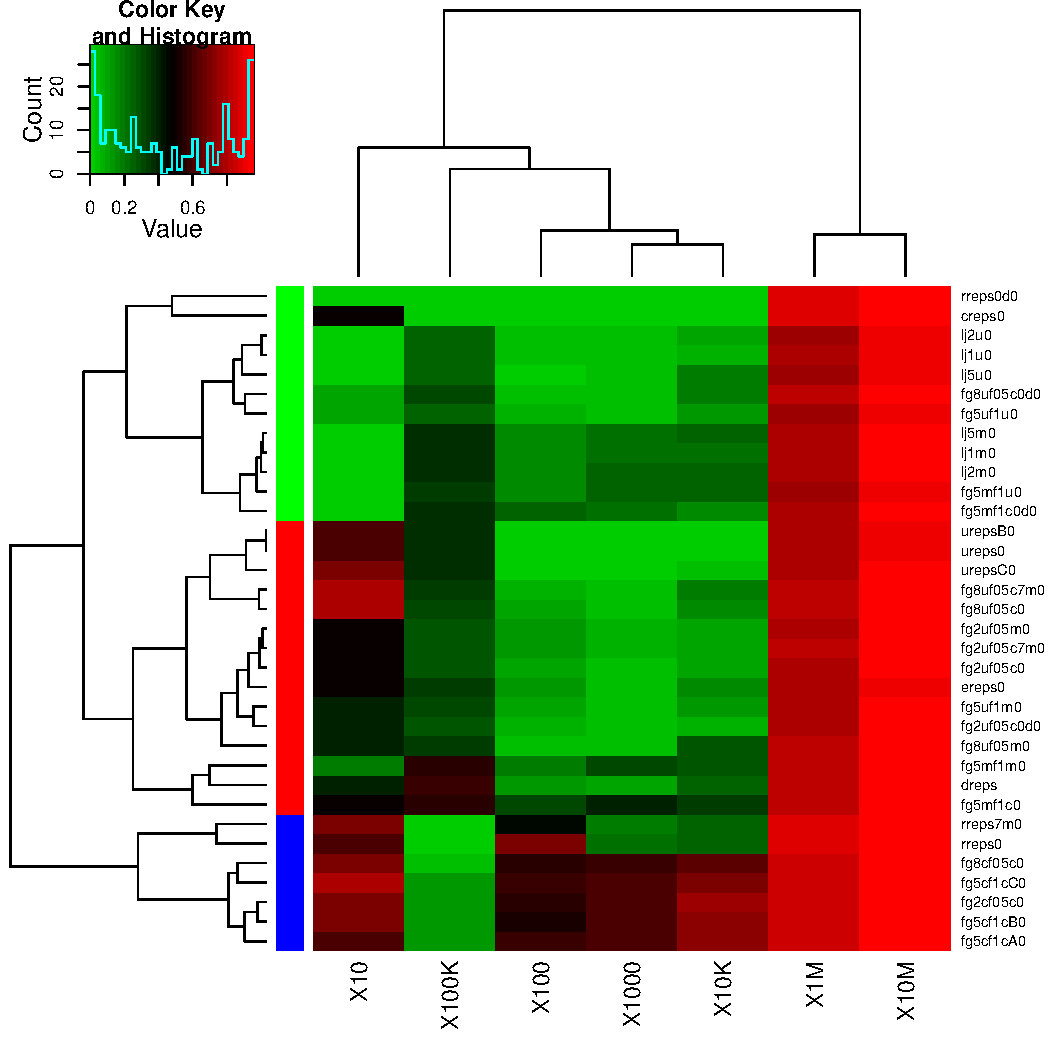
\includegraphics{figures/heatmap-overx-dreps-medians-0wk}
    \caption{Reality overlap clustering of all simulations started from scratch.}
    \label{figure:heatmap-overx-dreps-medians-0wk}
\end{center}
\end{figure}
Figure~\ref{figure:heatmap-overx-dreps-medians-1wk} shows reality overlap clustering of all of the basic simulations, run after mixing in one week of the {\itshape dreps} reality itself.


The bucketed simulations join in, and while those modifying only small elice buckets, {\itshape {1,2,3}f}, are predictably close to reality, so is {\itshape 6f}, simulating the complete one million strong middle class with the capital-capital strategy, {\itshape fg5cf1c}.



\begin{figure}
\begin{center}
    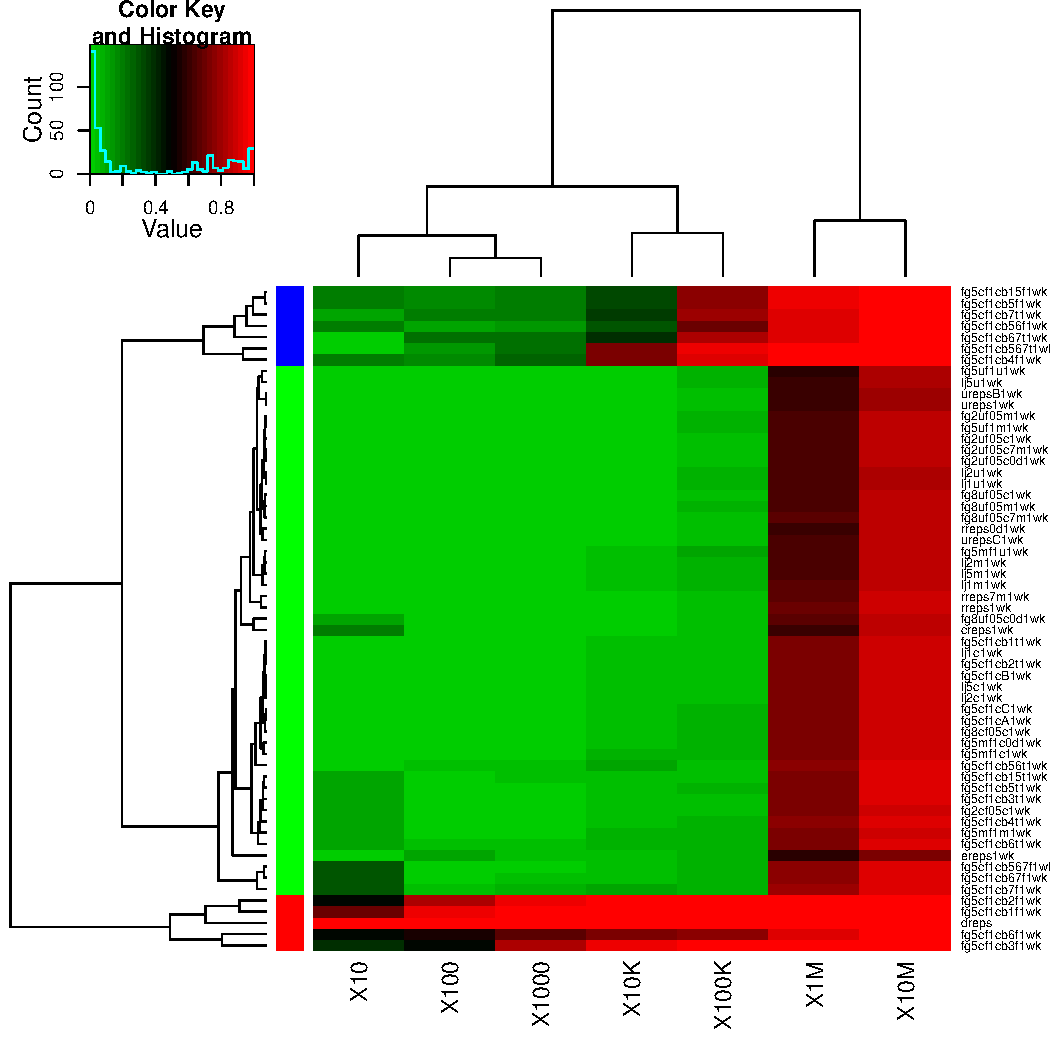
\includegraphics{figures/heatmap-overx-dreps-medians-1wk}
    \caption{Reality overlap clustering of all simulations seeded by 1 week of reality.}
    \label{figure:heatmap-overx-dreps-medians-1wk}
\end{center}
\end{figure}
Figure~\ref{figure:heatmap-overx-dreps-medians-2wk} shows reality overlap clustering of all of the basic simulations, run after mixing in two weeks of the {\itshape dreps} reality itself.


The bucketed middle class stays close to reality here as well.


We also see increasing capture of the celebrity class, top ten, by both bucketed and non-bucketed simulations, specifically


\begin{itemize}


\item creps2wk

\item fg8uf05m2wk
\end{itemize}


\begin{figure}
\begin{center}
    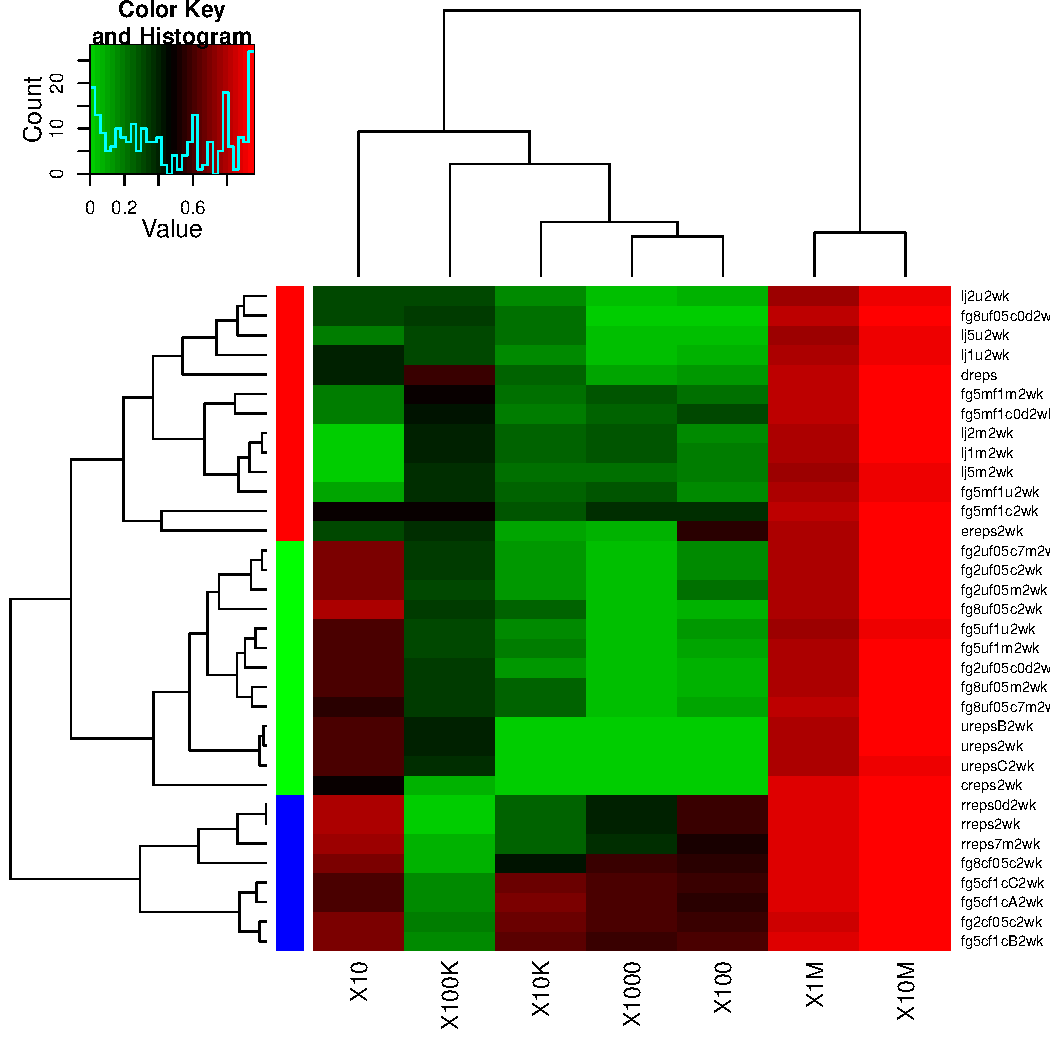
\includegraphics{figures/heatmap-overx-dreps-medians-2wk}
    \caption{Reality overlap clustering of all simulations seeded by 2 weeks of reality.}
    \label{figure:heatmap-overx-dreps-medians-2wk}
\end{center}
\end{figure}
Figure~\ref{figure:heatmap-overx-dreps-medians-3wk} shows reality overlap clustering of all of the basic simulations, run after mixing in three weeks of the {\itshape dreps} reality itself.


The simulated middle class remains really close to reality, and celebrities are captured better in most of the simuations, except the uniform {\itshape ureps} runs.
Notably, the mentions-mentions strategy with 0.5 utility probability does well:


\begin{itemize}


\item fg5m1m
\end{itemize}


\begin{figure}
\begin{center}
    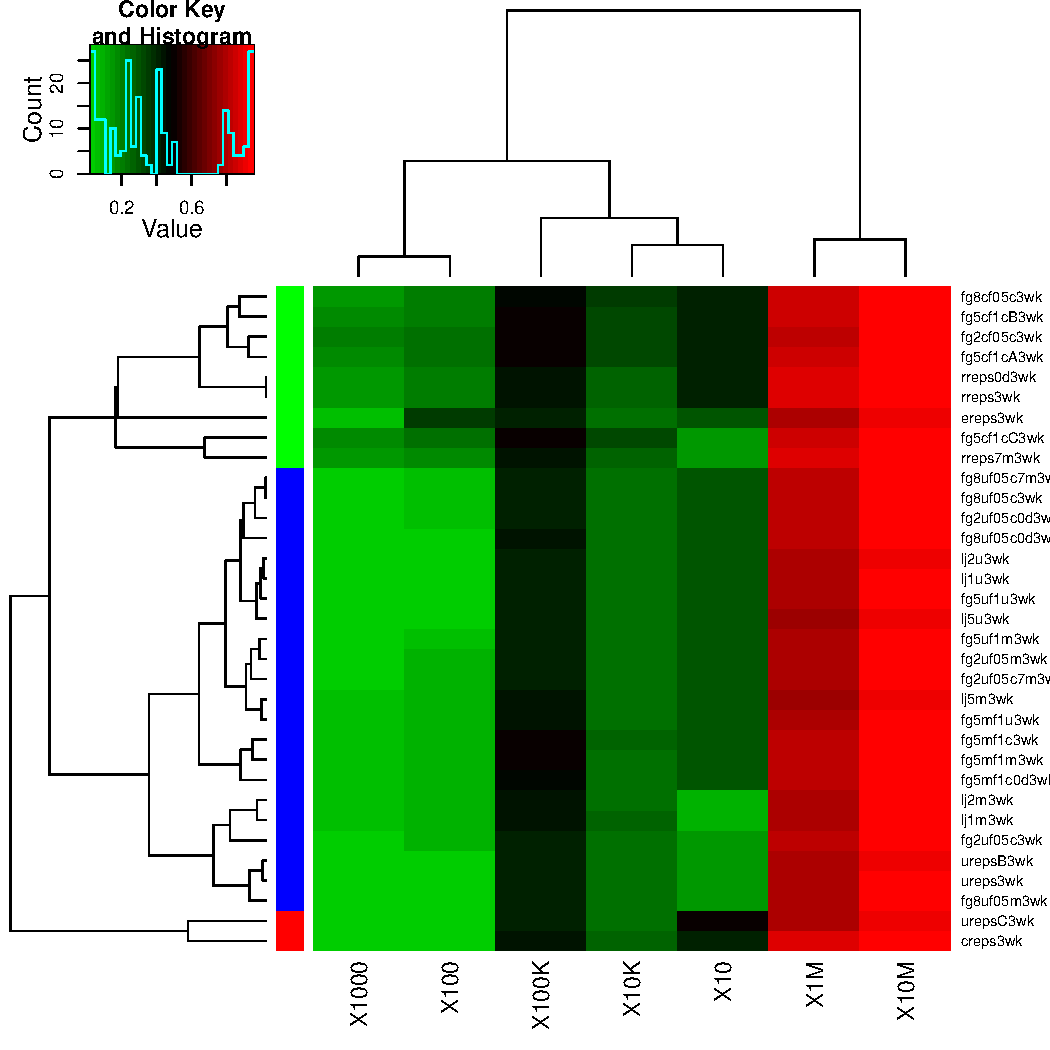
\includegraphics{figures/heatmap-overx-dreps-medians-3wk}
    \caption{Reality overlap clustering of all simulations seeded by 3 weeks of reality.}
    \label{figure:heatmap-overx-dreps-medians-3wk}
\end{center}
\end{figure}
\pagebreak \subsection{Overlap with Self, Reality-shifted}
\label{overlapwithselfreality-shifted}

For all simulations with several runs differing only by the amount of reality seeding, we compute the overlap of social wealth hierarchies, between the simulations separated by a week of reality, with as many steps as there are such pairs.  It usually means 4 pairs for non-bucketed, or 2 pairs for bucketed simulations.


Capital-capital FOF-based simulations show pretty good stability right away --- Figure~\ref{figure:heatmap-overx-self-medians-0wk}, --- with especially strong showing in the 1,000 elite bucket and the middle class.


{\itshape Rrreps} and {\itshape creps} do well in the upper-middle class while FOF-based, uniform global strategies capture the celebrity bucket.


The pattern continues into the first $\rightarrow$ second week pair --- Figure~\ref{figure:heatmap-overx-self-medians-1wk}, --- where non-bucketed capital-based simulations, both FOF and non-FOF utility based, bring up the middle considerably.  The newly arrived bucketed simulations do especially well, of course.  This continues into the second $\rightarrow$ third week --- Figure~\ref{figure:heatmap-overx-self-medians-2wk} --- and third $\rightarrow$ fourth --- Figure~\ref{figure:heatmap-overx-self-medians-3wk} --- pairs as well.



\begin{figure}
\begin{center}
    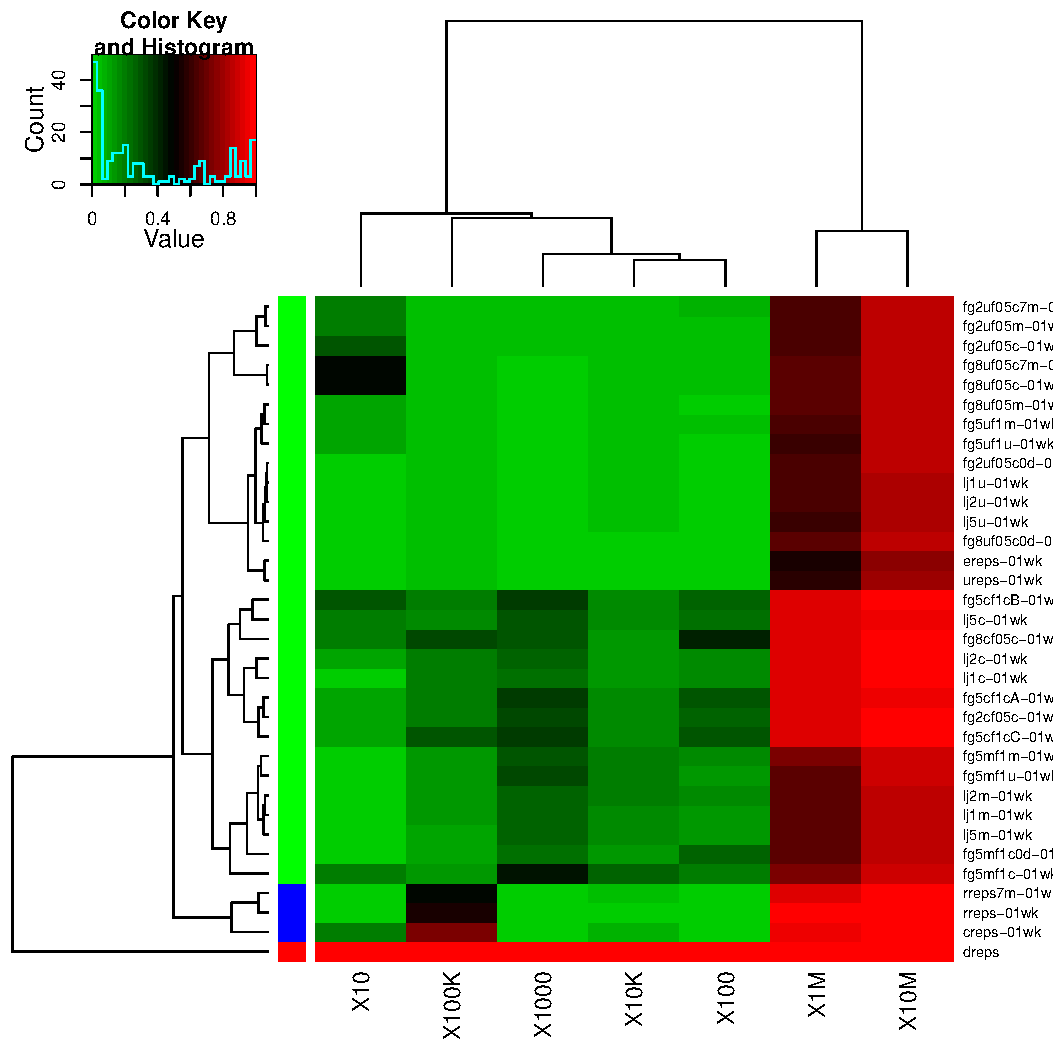
\includegraphics{figures/heatmap-overx-self-medians-0wk}
    \caption{Overlap with the same strategy seeded by one more week of reality, 0 vs 1 week.}
    \label{figure:heatmap-overx-self-medians-0wk}
\end{center}
\end{figure}

\begin{figure}
\begin{center}
    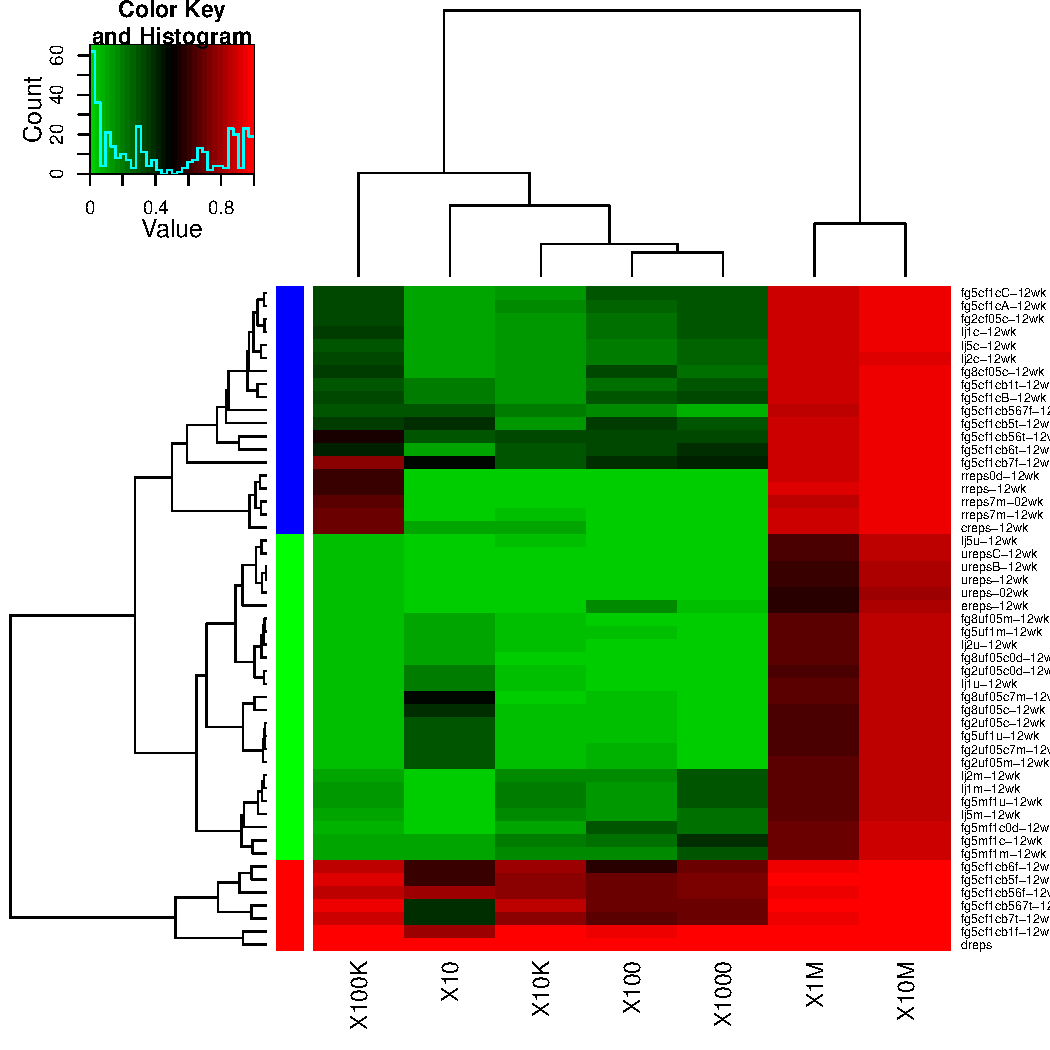
\includegraphics{figures/heatmap-overx-self-medians-1wk}
    \caption{Overlap with the same strategy seeded by one more week of reality, 1 vs 2 weeks.}
    \label{figure:heatmap-overx-self-medians-1wk}
\end{center}
\end{figure}

\begin{figure}
\begin{center}
    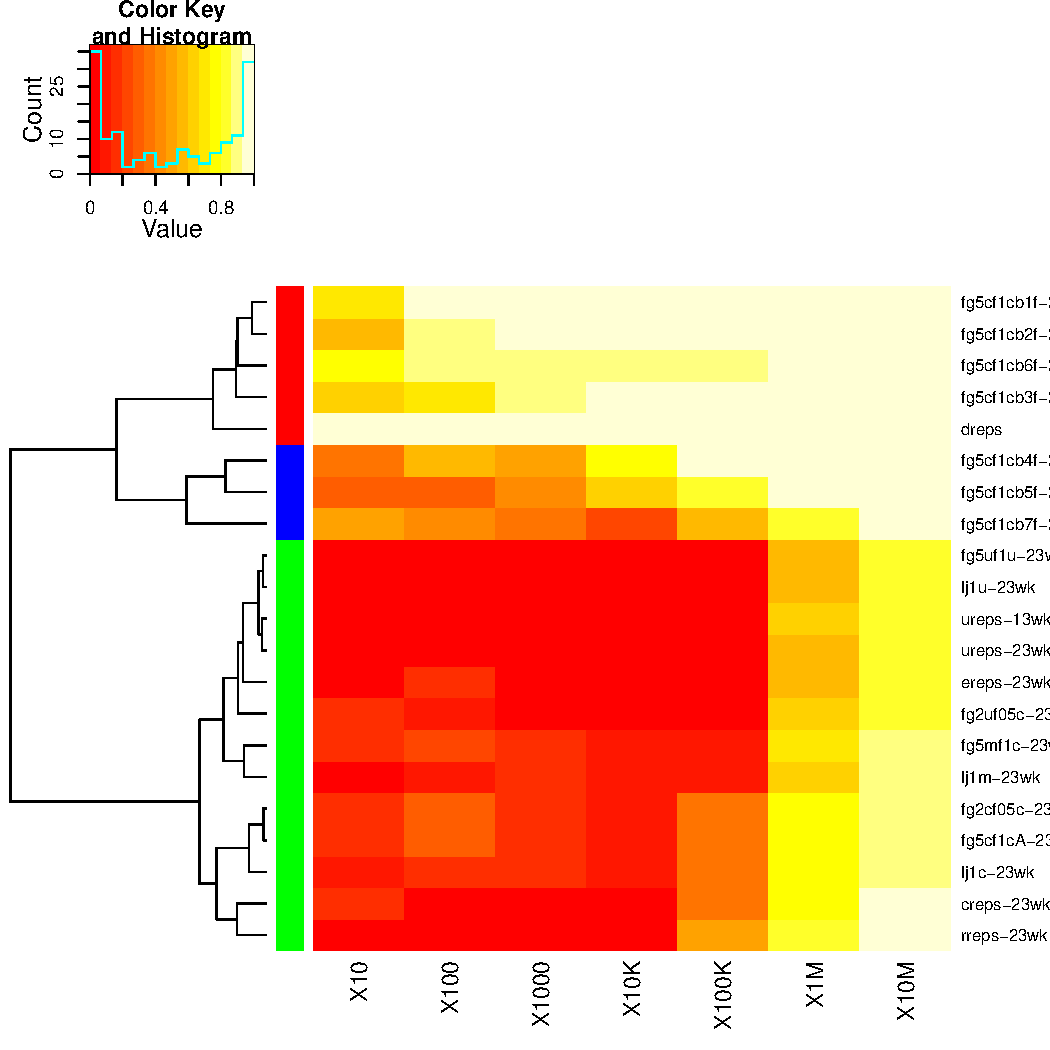
\includegraphics{figures/heatmap-overx-self-medians-2wk}
    \caption{Overlap with the same strategy seeded by one more week of reality, 2 vs 3 weeks.}
    \label{figure:heatmap-overx-self-medians-2wk}
\end{center}
\end{figure}

\begin{figure}
\begin{center}
    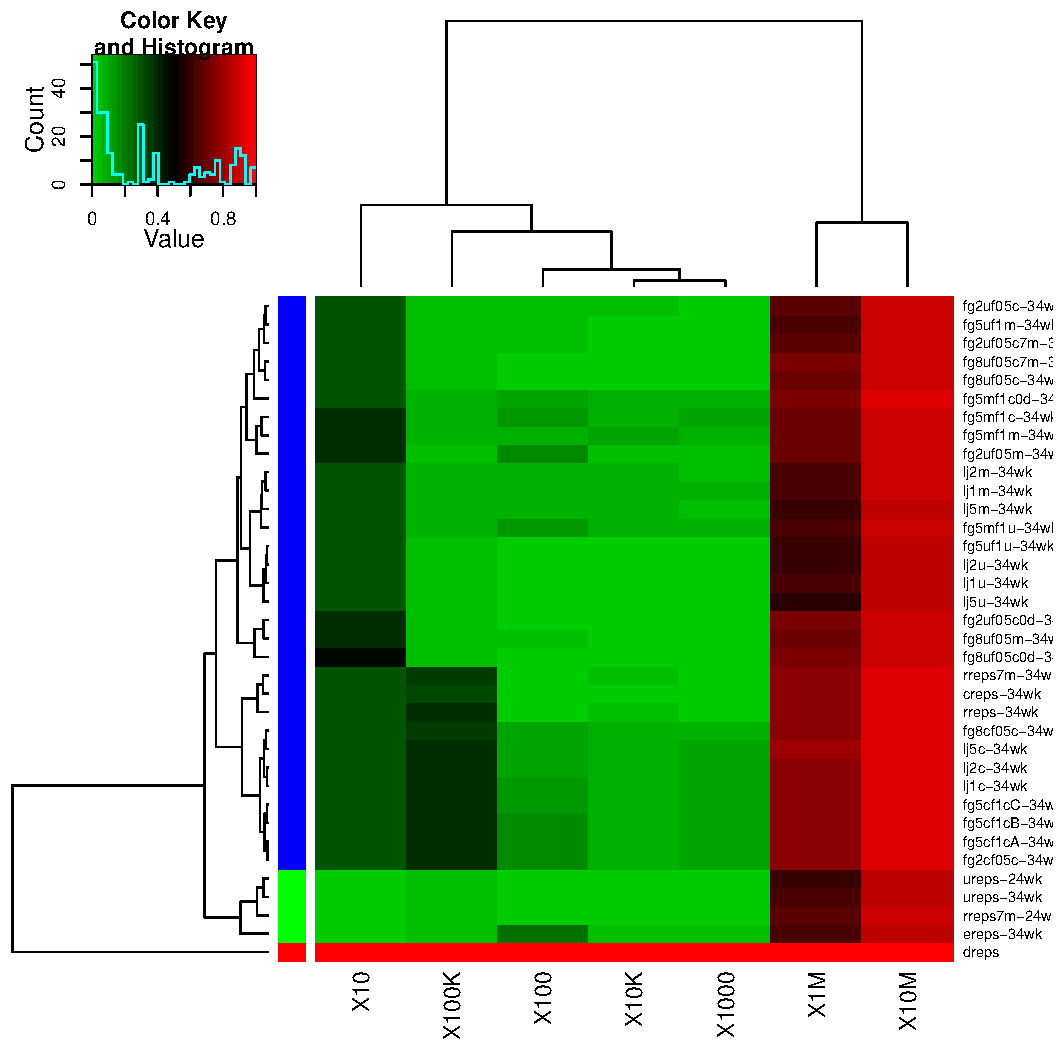
\includegraphics{figures/heatmap-overx-self-medians-3wk}
    \caption{Overlap with the same strategy seeded by one more week of reality, 3 vs 4 weeks.}
    \label{figure:heatmap-overx-self-medians-3wk}
\end{center}
\end{figure}
\pagebreak \subsection{Staying Rates}
\label{stayingrates}

Figures \ref{figure:heatmap-srates-medians-0wk},\ref{figure:heatmap-srates-medians-1wk},\ref{figure:heatmap-srates-medians-2wk},\ref{figure:heatmap-srates-medians-3wk} show the evolution of staying power as the amount of reality seeding increases.  


Uniform global strategies coupled with capital-based {\itshape FOF} ones are closer to {\itshape dreps} initially, then mentions-based global ones get closer, and finally capital-capital ones dominate.  It shows that effective communication gets closer to reality when seeded with more history of such communication.


Figure~\ref{figure:heatmap-srates-medians-0wk} shows staying power clustering of all of the basic simulations, run from scratch without mixing any of the {\itshape dreps} reality.


Several {\itshape freps} simulations are near {\itshape dreps}, notably fg8uf05m0 and fg5uf1m0.  Also {\itshape ereps0} is not far.  Capital-capital ones are in a separate cluster.



\begin{figure}
\begin{center}
    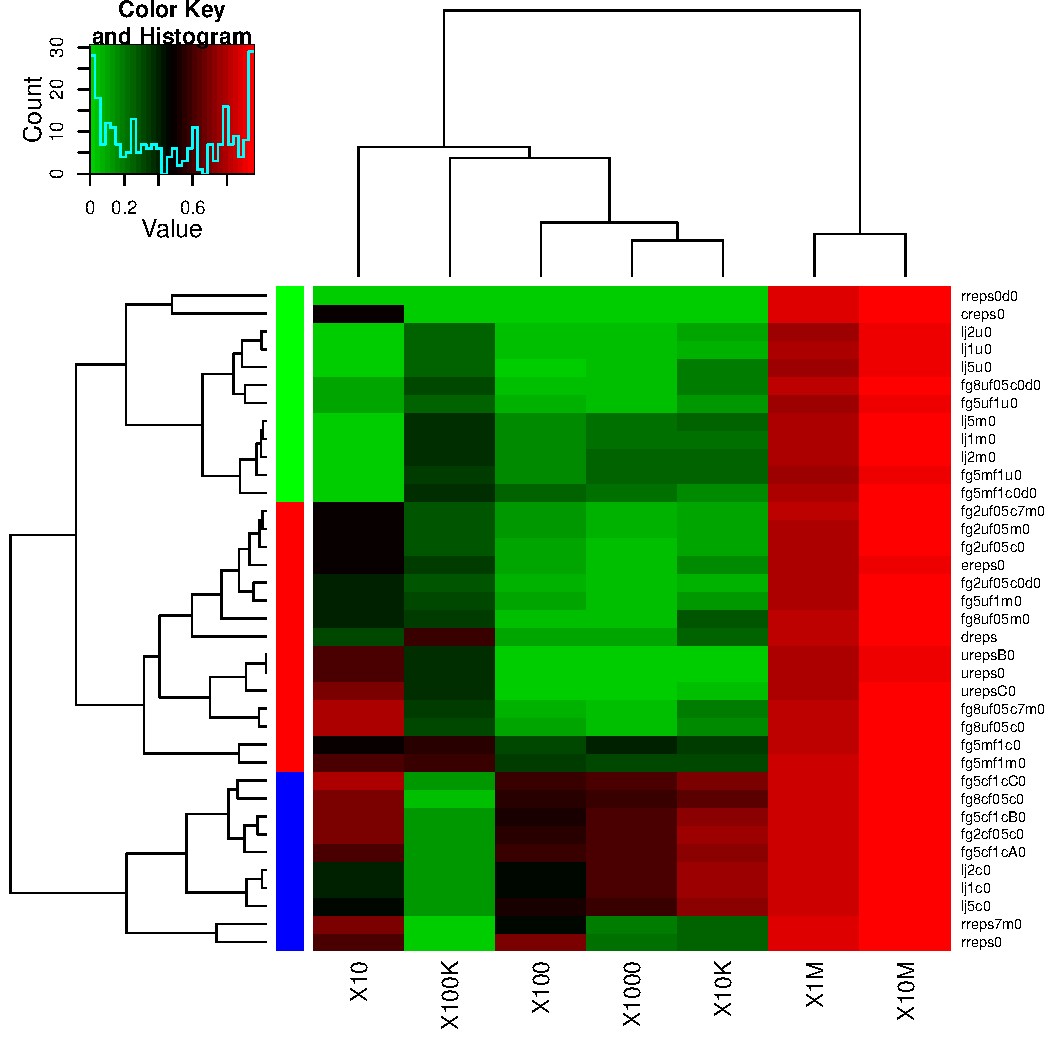
\includegraphics{figures/heatmap-srates-medians-0wk}
    \caption{Staying power clustering of all simulations started from scratch.}
    \label{figure:heatmap-srates-medians-0wk}
\end{center}
\end{figure}
Figure~\ref{figure:heatmap-srates-medians-1wk} shows staying power clustering of all of the basic simulations, seeded with one week of the {\itshape dreps} reality.


Bucketed middle class simulation, {\itshape 6f}, is close, and {\itshape ereps}\_ is not far again.  Simulated celebrities, {\itshape 1f}, are in a separate cluster.  {\itshape 2f} is next to {\itshape dreps}, and {\itshape fg5mf1c} and {\itshape fg5mf1m} are next.



\begin{figure}
\begin{center}
    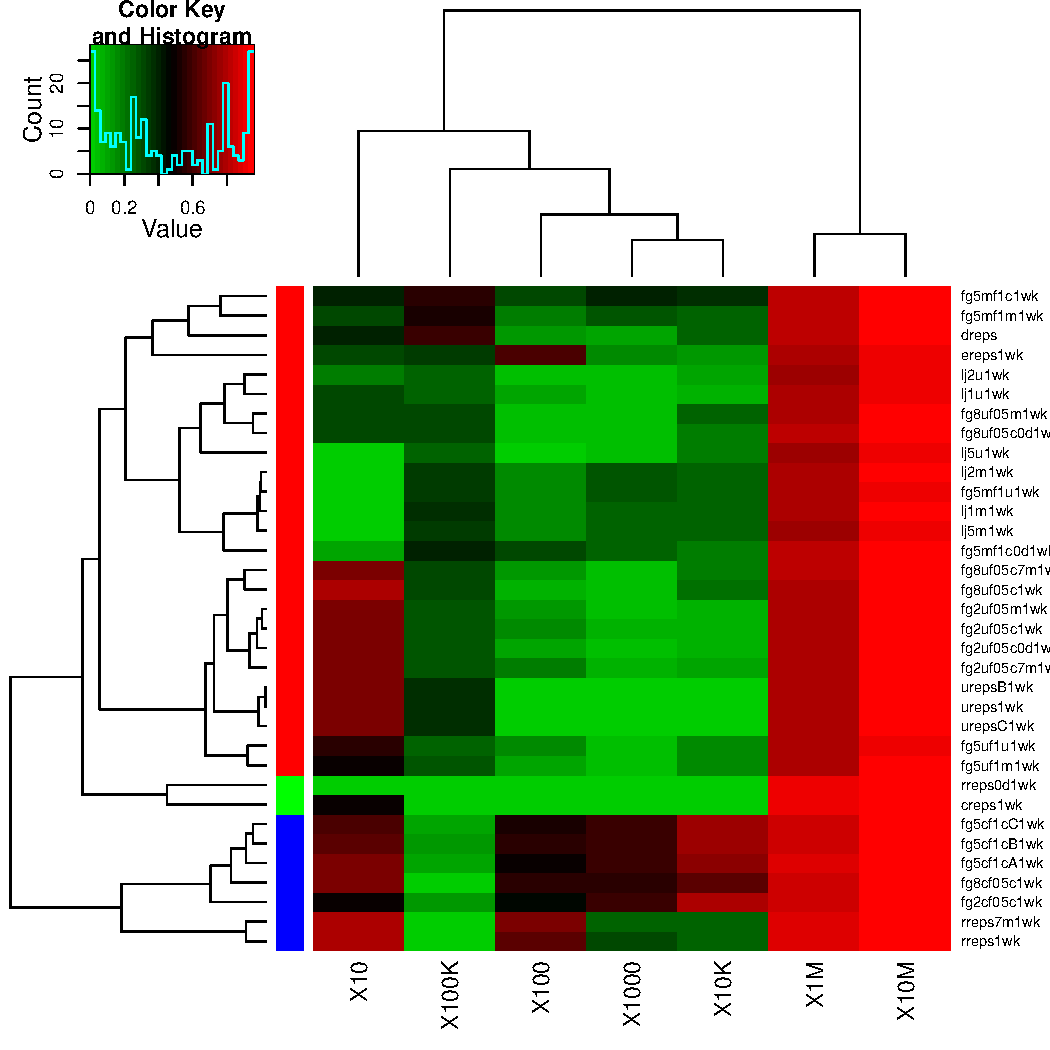
\includegraphics{figures/heatmap-srates-medians-1wk}
    \caption{Staying power clustering of all simulations seeded by 1 week of reality.}
    \label{figure:heatmap-srates-medians-1wk}
\end{center}
\end{figure}
Figure~\ref{figure:heatmap-srates-medians-2wk} shows staying power clustering of all of the basic simulations, seeded with two weeks of the {\itshape dreps} reality.


The bucketed ones are the closest as usual -- {\itshape 2f}, {\itshape 15f}.  Then we have 


\begin{itemize}


\item {\itshape lj{1,5,2}u}

\item {\itshape fg8uf05c0d}


{\itshape 6f} is further in the cluster, next to {\itshape 1f}.



\end{itemize}


\begin{figure}
\begin{center}
    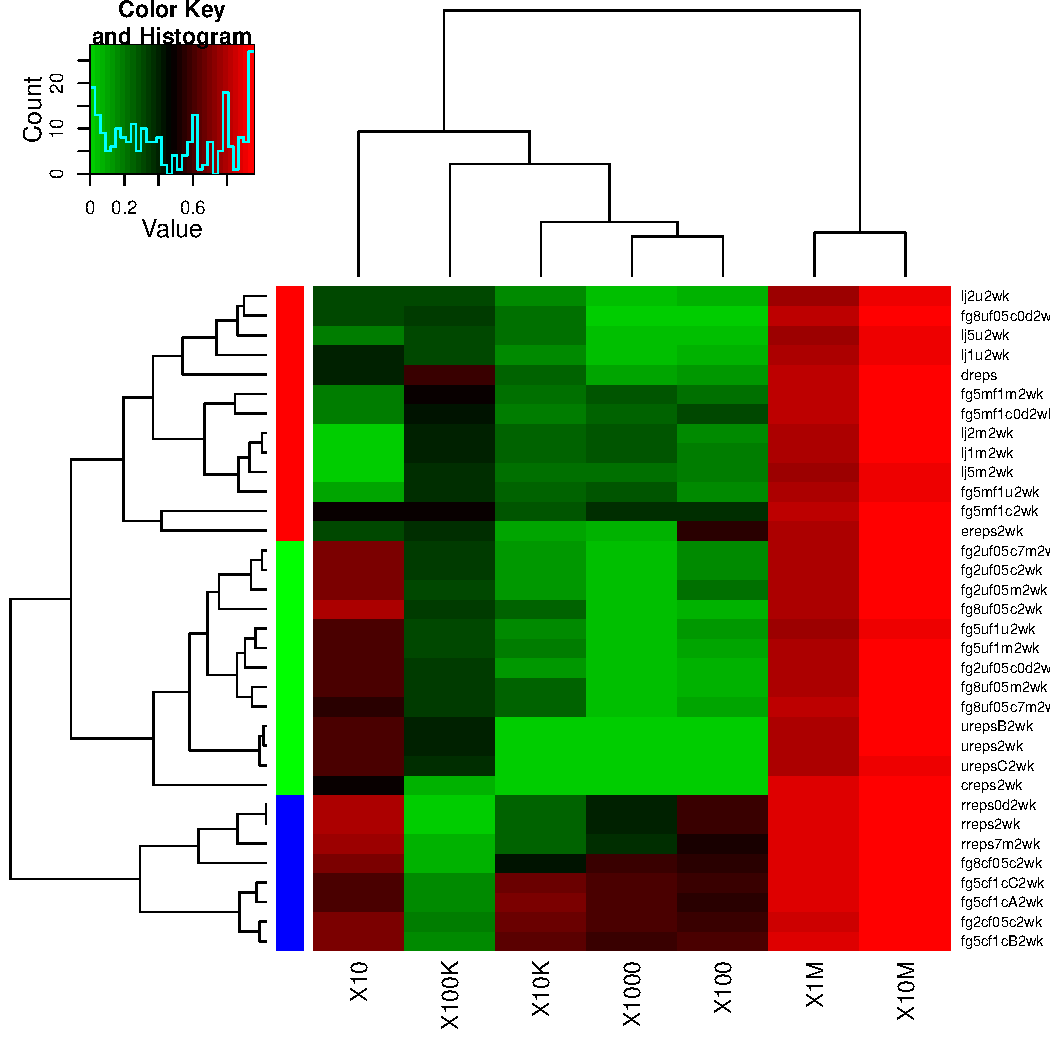
\includegraphics{figures/heatmap-srates-medians-2wk}
    \caption{Staying power clustering of all simulations seeded by 2 weeks of reality.}
    \label{figure:heatmap-srates-medians-2wk}
\end{center}
\end{figure}
Figure~\ref{figure:heatmap-srates-medians-3wk} shows staying power clustering of all of the basic simulations, seeded with two weeks of the {\itshape dreps} reality.


The bucketed are now bracketing reality, with the middle class {\itshape 6f} one of the closest.  Among the closest nonbucketed ones are


\begin{itemize}


\item {\itshape fg5cf1cC}

\item {\itshape rreps7m}

\item {\itshape ereps}
\end{itemize}

\pagebreak \subsection{Volumes per Bucket}
\label{volumesperbucket}

\subsubsection{Volume of Replies}
\label{volumeofreplies}

Volume of replies per bucket follows mostly the same pattern, shown here as a barplot of the medians per bucket, across all simulations.   Not the main unexpected feature here -- the middle class contributes practically as much as all the poor, combined, about 40\% of all replies.



\begin{figure}
\begin{center}
    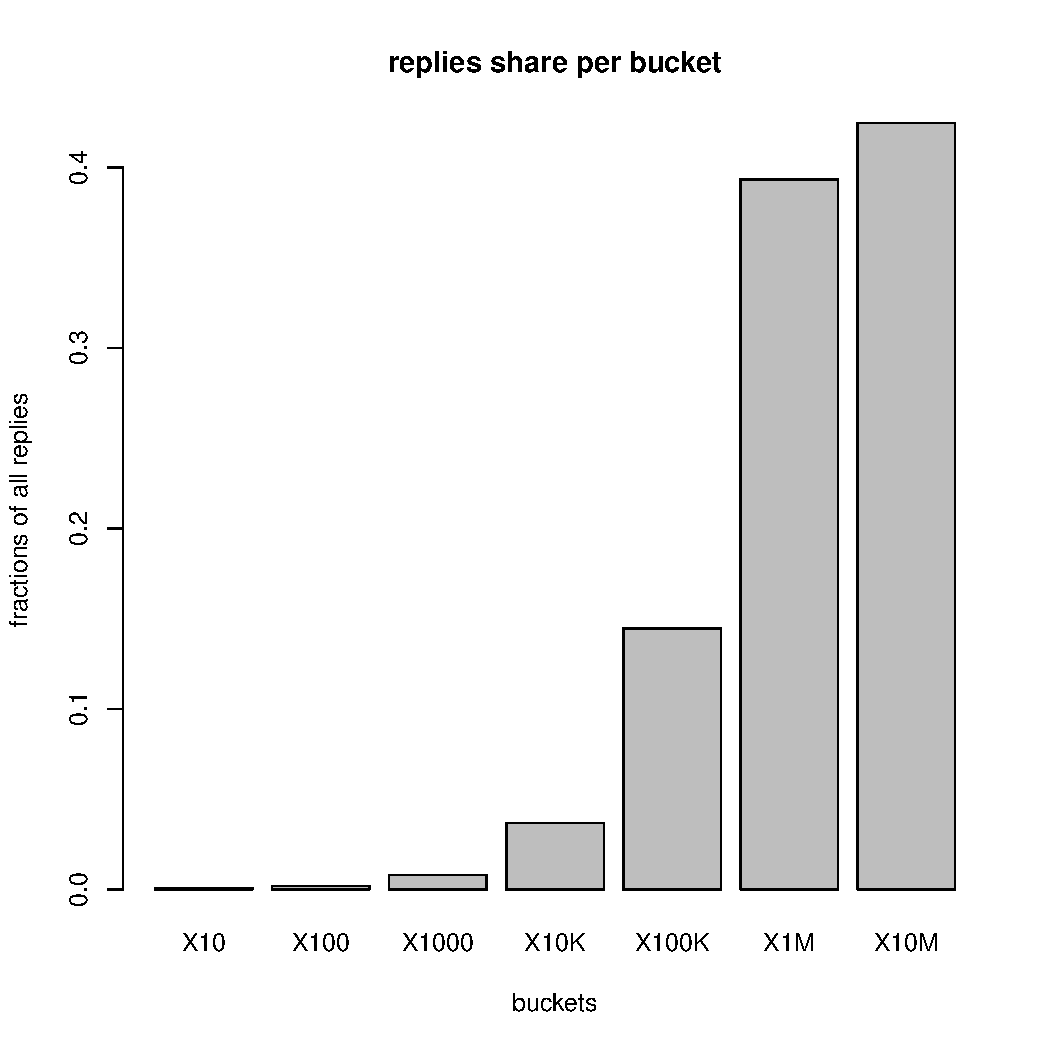
\includegraphics[width=4in]{figures/vols4-re-norm-medians-med}
    \caption{Medians of all bucket reply shares, for all simulations, per bucket.}
    \label{figure:vols4-re-norm-medians-med}
\end{center}
\end{figure}
\pagebreak \subsubsection{Volume of Mentions}
\label{volumeofmentions}

Figure~\ref{figure:heatmap-vols4-me-norm-medians-0wk} shows per-bucket volume of mentions (incoming communications) for all simulations  run from scratch without mixing any of the {\itshape dreps} reality (which do not contain the bucketed ones as one week at least is required to mature the social capital).


Initially, strategies with a smaller utility probability are closer to reality, along with global mentions, pure or combined.



\begin{figure}
\begin{center}
    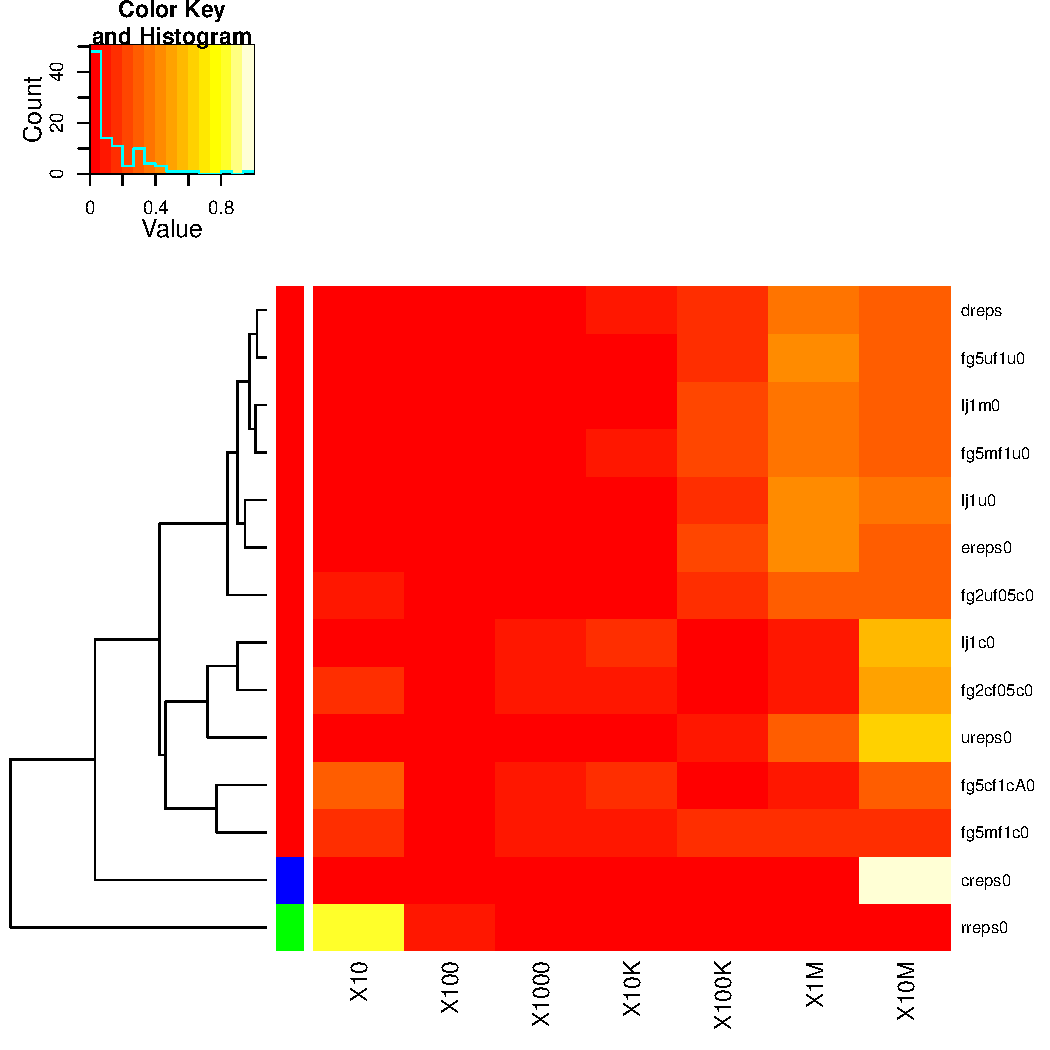
\includegraphics{figures/heatmap-vols4-me-norm-medians-0wk}
    \caption{Per-bucket mentions volume for all simulations started from scratch.}
    \label{figure:heatmap-vols4-me-norm-medians-0wk}
\end{center}
\end{figure}
Figure~\ref{figure:heatmap-vols4-me-norm-medians-1wk} shows per-bucket volume of mentions (incoming communications) for all of the simulations, seeded with one week of the {\itshape dreps} reality.


Once the bucketed kick in, we have the usual elite-changing ones clustering around reality, with middle class, {\itshape preserved} --- {\itshape 6t} --- nearby, as well as two FOF-based with {\itshape jumpProbUtil} of 0.5, and global mentions with utility:


\begin{itemize}


\item fg5uf1u

\item fg5mf1u

\item lj5m
\end{itemize}


\begin{figure}
\begin{center}
    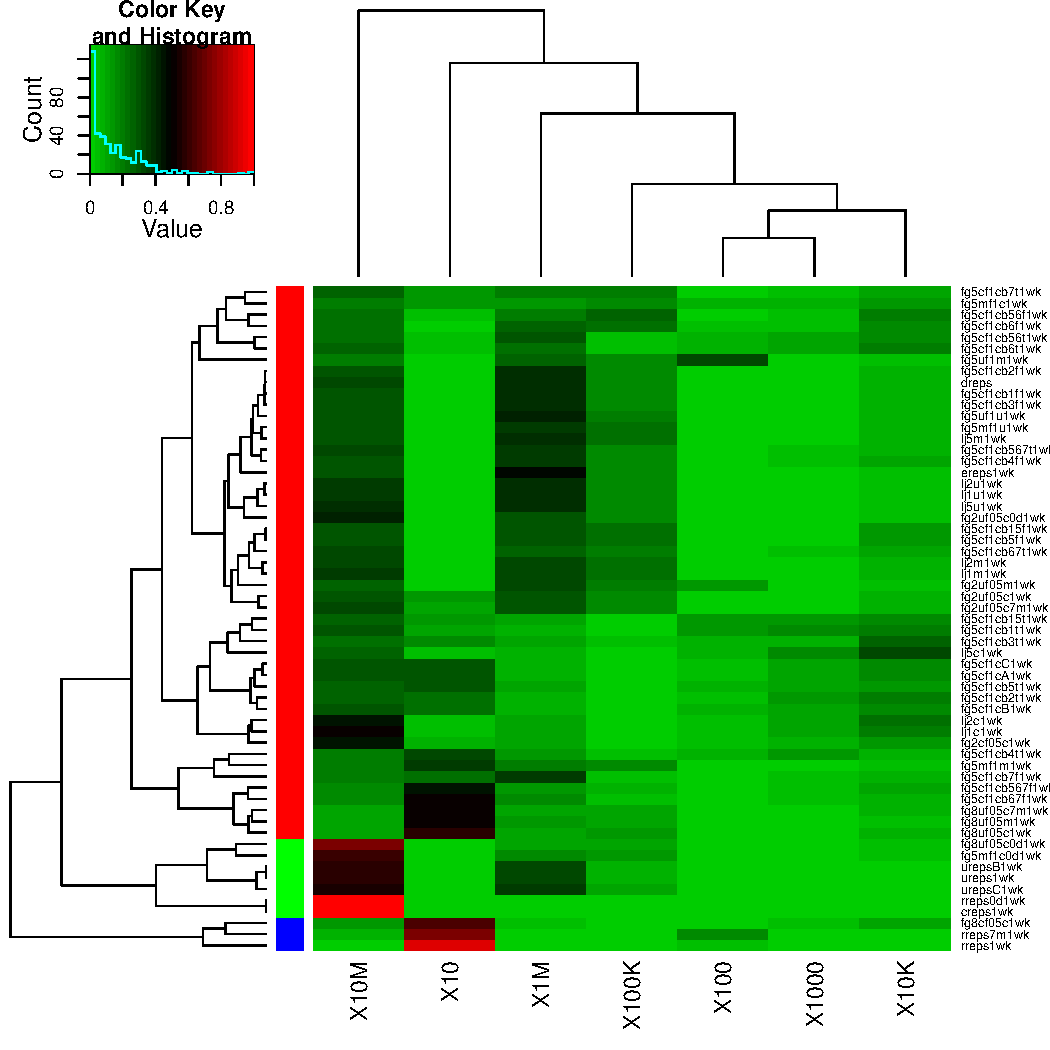
\includegraphics{figures/heatmap-vols4-me-norm-medians-1wk}
    \caption{Per-bucket mentions volume for all simulations seeded by 1 week of reality.}
    \label{figure:heatmap-vols4-me-norm-medians-1wk}
\end{center}
\end{figure}
Figure~\ref{figure:heatmap-vols4-me-norm-medians-2wk} shows per-bucket volume of mentions (incoming communications) for all of the simulations, seeded with two weeks of the {\itshape dreps} reality.


Bucketed align around {\itshape dreps} in the usual formation, with the previously noted non-bucketed ones staying around:


\begin{itemize}


\item fg5mf1u

\item lj5m
\end{itemize}

The simulated middle class is near the opposite combination, global uniform after FOF-mentions, in another subcluster of {\itshape dreps}:


\begin{itemize}


\item fg5cf1cb6f

\item fg5uf1m
\end{itemize}


\begin{figure}
\begin{center}
    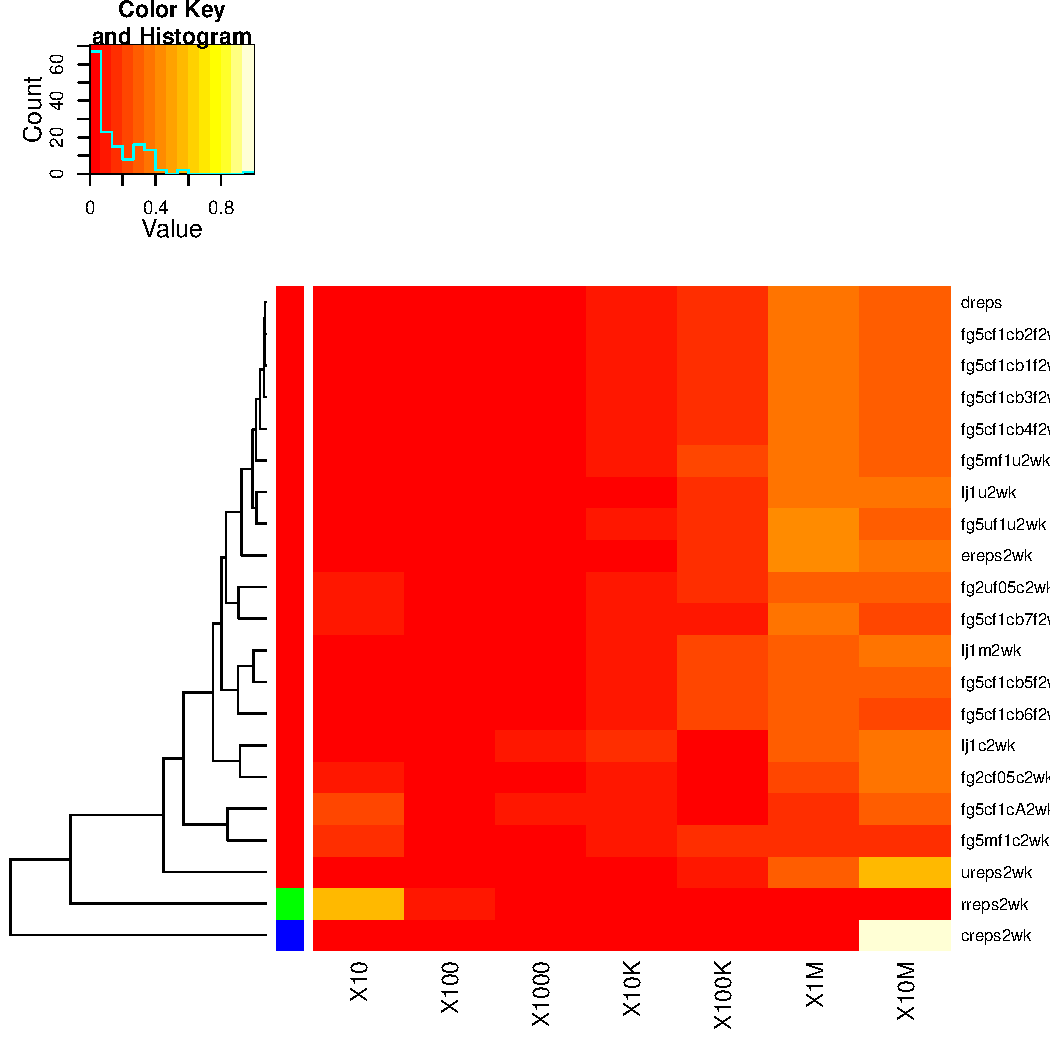
\includegraphics{figures/heatmap-vols4-me-norm-medians-2wk}
    \caption{Per-bucket mentions volume for all simulations seeded by 2 weeks of reality.}
    \label{figure:heatmap-vols4-me-norm-medians-2wk}
\end{center}
\end{figure}
Figure~\ref{figure:heatmap-vols4-me-norm-medians-3wk} shows per-bucket volume of mentions (incoming communications) for all of the simulations, seeded with three weeks of the {\itshape dreps} reality.


Finally, fractions look quite similar.  Clustering keeps our early non-bucketed close:


\begin{itemize}


\item fg5mf1u

\item lj5m
\end{itemize}

The simulated middle class is in a separate cluster since it underestimates the poor, while the preserved one does better.



\begin{figure}
\begin{center}
    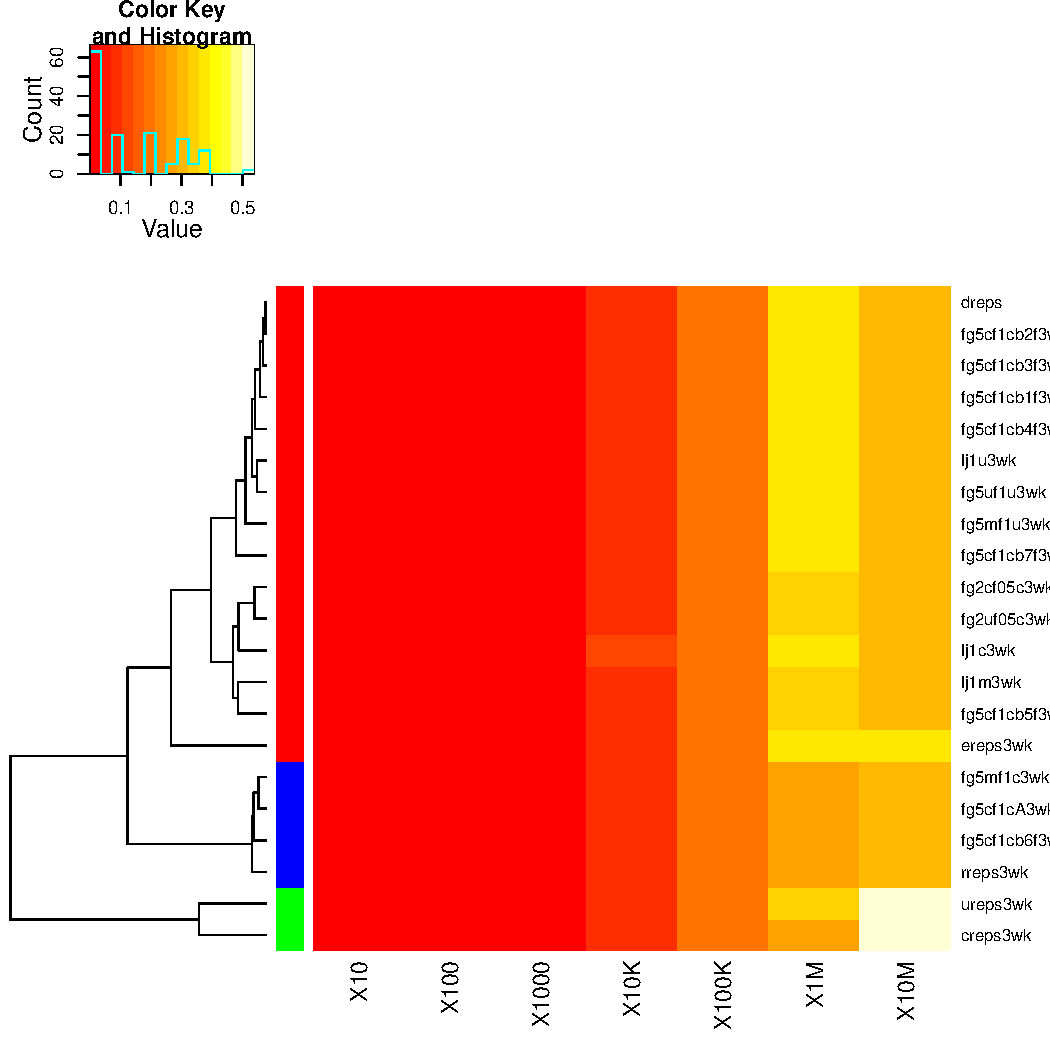
\includegraphics{figures/heatmap-vols4-me-norm-medians-3wk}
    \caption{Per-bucket mentions volume for all simulations seeded by 3 weeks of reality.}
    \label{figure:heatmap-vols4-me-norm-medians-3wk}
\end{center}
\end{figure}
\pagebreak \subsection{Starranks}
\label{starranks}

Starranks are ratios, and as such fall into a wider range than overlaps or volumes, which are simple fractions from 0 to 1.  In order to compare the differences in starranks per buckets, ranging widely, we operate with $\log10$ of starranks.  It also clearly shows how lower classes generally talk to a higher-ranked audience, while the top classes talk to the lower-ranked ones.


\pagebreak \subsubsection{Starranks for Mentions}
\label{starranksformentions}

We cluster median starranks per bucket, aggregated as overall medians for all days of each simulation, by distance from each other and {\itshape dreps}, the reality.  We segment the simulations by the amount of reality used to seed them, into four overall classes -- 0, 1wk, 2wk, and 3wk.


Figure~\ref{figure:heatmap-sbucks-ments-star-med-medians-0wk} shows the median starranks, based on the ratios of one's social capital over the weighted average of one's audience's, per-bucket for mentions (incoming communications), for all simulations run from scratch without mixing any of the {\itshape dreps} reality (which do not contain the bucketed ones as one week at least is required to mature the social capital).


Capital-capital simulations are a majority in the {\itshape dreps} cluster.



\begin{figure}
\begin{center}
    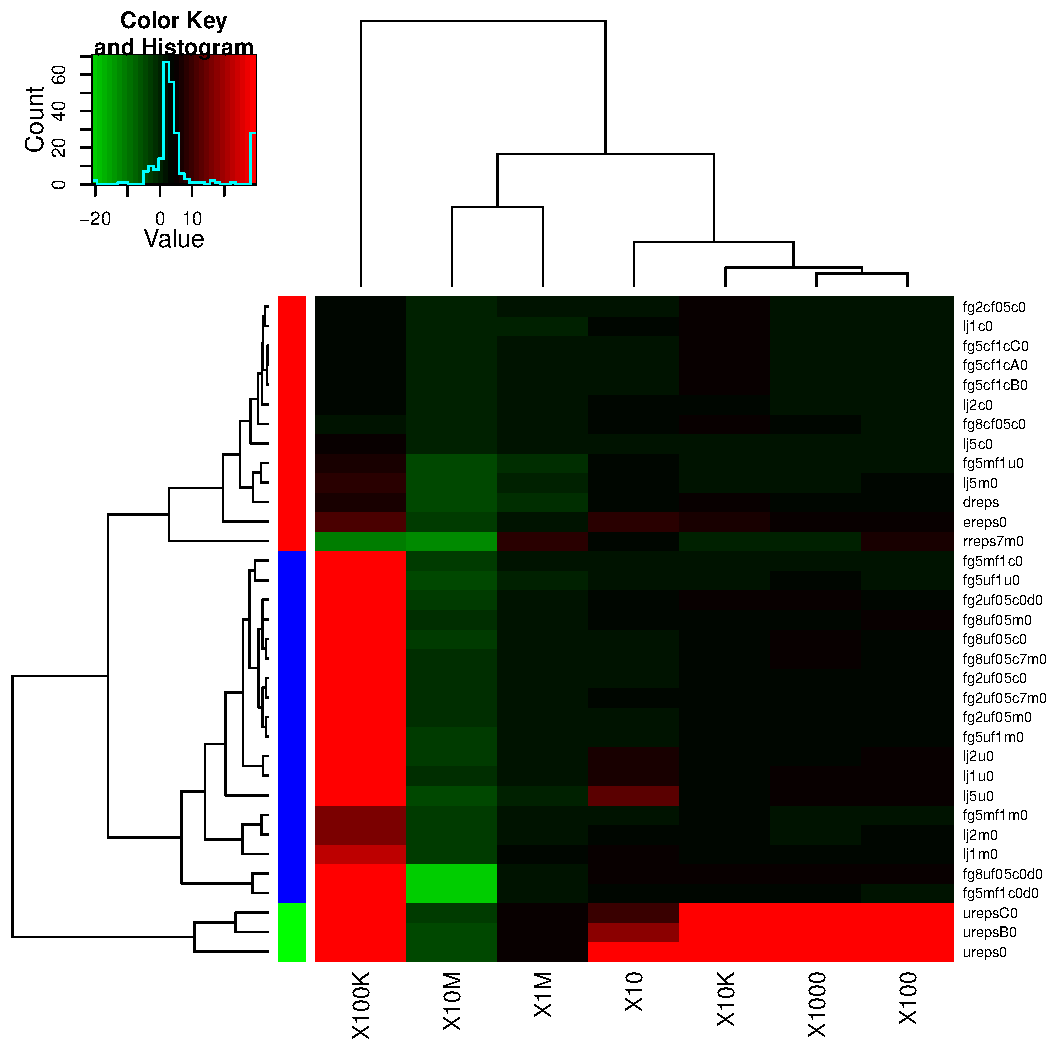
\includegraphics{figures/heatmap-sbucks-ments-star-med-medians-0wk}
    \caption{Starranks by mentions for all simulations started from scratch.}
    \label{figure:heatmap-sbucks-ments-star-med-medians-0wk}
\end{center}
\end{figure}
Figure~\ref{figure:heatmap-sbucks-ments-star-med-medians-1wk} shows median starranks, based on the ratios of one's social capital over the weighted average of one's audience's, per-bucket for mentions (incoming communications) for all of the simulations, seeded with one week of the {\itshape dreps} reality.


The bucketed simulations changing only the smaller, elite buckets are naturally closer here; {\itshape ereps1wk} is a notable closest non-bucketed one.


Interestingly, keeping or redoing the middle class, {\itshape 6t/6f}, ends up close together, showing that the middle class is well approximated by the underlying capital-capital FOF-based strategy.


We have a block of high starrank in upper middle class, for many simulations containing a global uniform strategy (and a couple of mentions-based one).



\begin{figure}
\begin{center}
    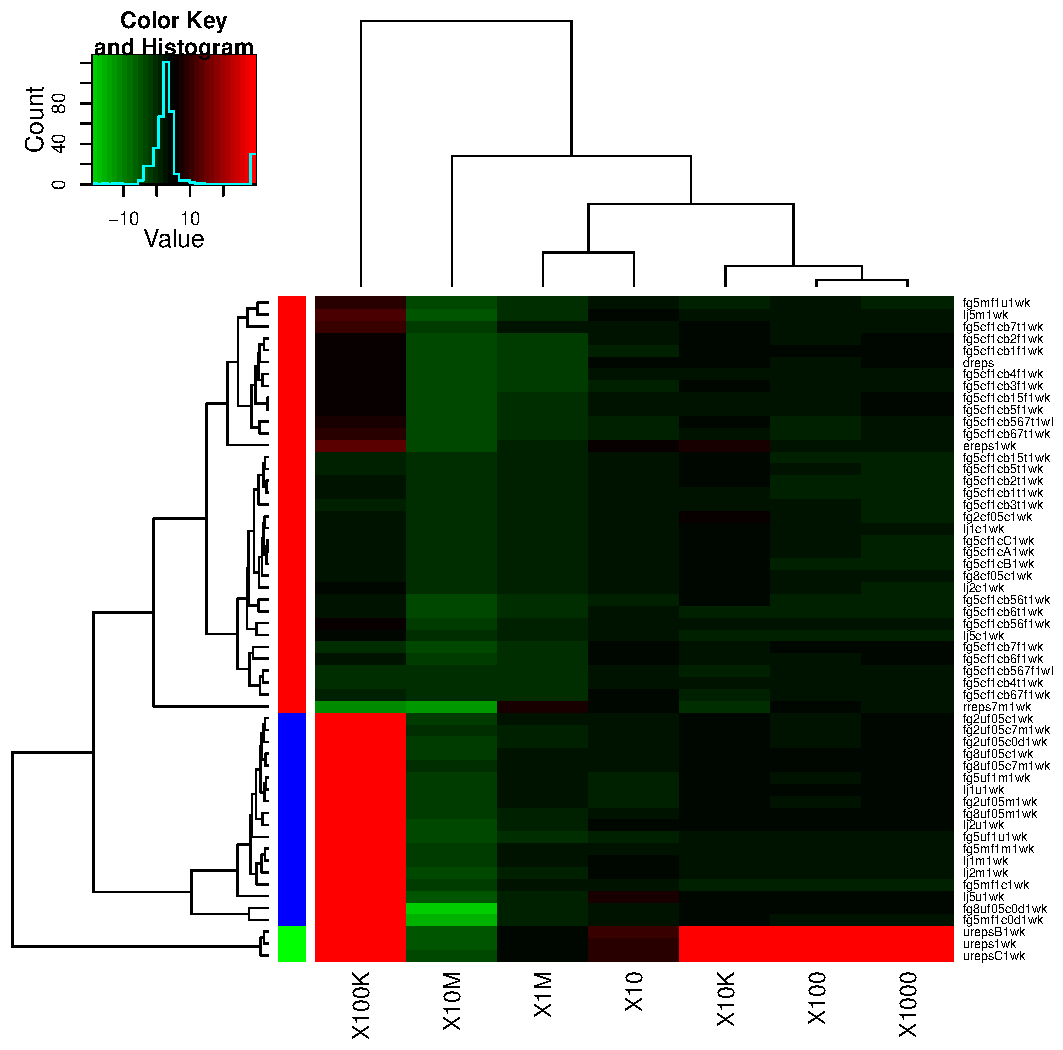
\includegraphics{figures/heatmap-sbucks-ments-star-med-medians-1wk}
    \caption{Starranks by mentions for all simulations seeded by 1 week of reality.}
    \label{figure:heatmap-sbucks-ments-star-med-medians-1wk}
\end{center}
\end{figure}
Figure~\ref{figure:heatmap-sbucks-ments-star-med-medians-2wk} shows median starranks, based on the ratios of one's social capital over the weighted average of one's audience's, per-bucket for mentions (incoming communications) for all of the simulations, seeded with two weeks of the {\itshape dreps} reality.


The combination redoing the top 4 buckets, and keeping the 3 lower ones, {\itshape 567t}, is close to {\itshape dreps}, followed by {\itshape 67t}, while the poor by themselves, \_7t), are father away, showing that the middle class matters a lot.


We have a similar block of high starrank in upper middle class, for many simulations containing a global uniform strategy, only two of them FOF-capital based, with rather large jump probability away from local utility (0.5 and 0.8).



\begin{figure}
\begin{center}
    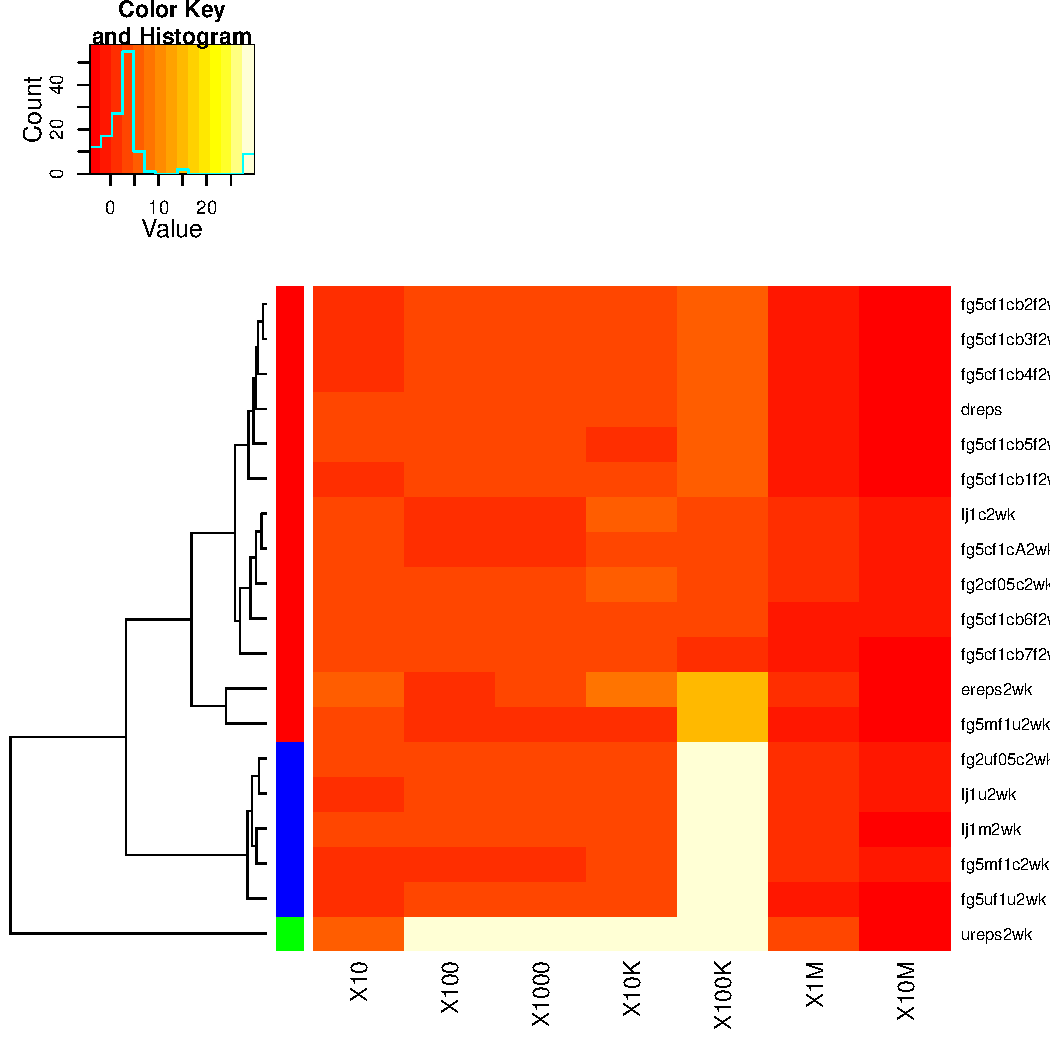
\includegraphics{figures/heatmap-sbucks-ments-star-med-medians-2wk}
    \caption{Starranks by mentions for all simulations seeded by 2 weeks of reality.}
    \label{figure:heatmap-sbucks-ments-star-med-medians-2wk}
\end{center}
\end{figure}
Figure~\ref{figure:heatmap-sbucks-ments-star-med-medians-3wk} shows median starranks, based on the ratios of one's social capital over the weighted average of one's audience's, per-bucket for mentions (incoming communications) for all of the simulations, seeded with three weeks of the {\itshape dreps} reality.


The range is shrinking here, from -2 to 6, while it exceeded the [-10,10] range for 1-2 weeks.


We have an even bigger block of simulations with extremely high starrank in the upper-middle class, now containing {\itshape dreps}.



\begin{figure}
\begin{center}
    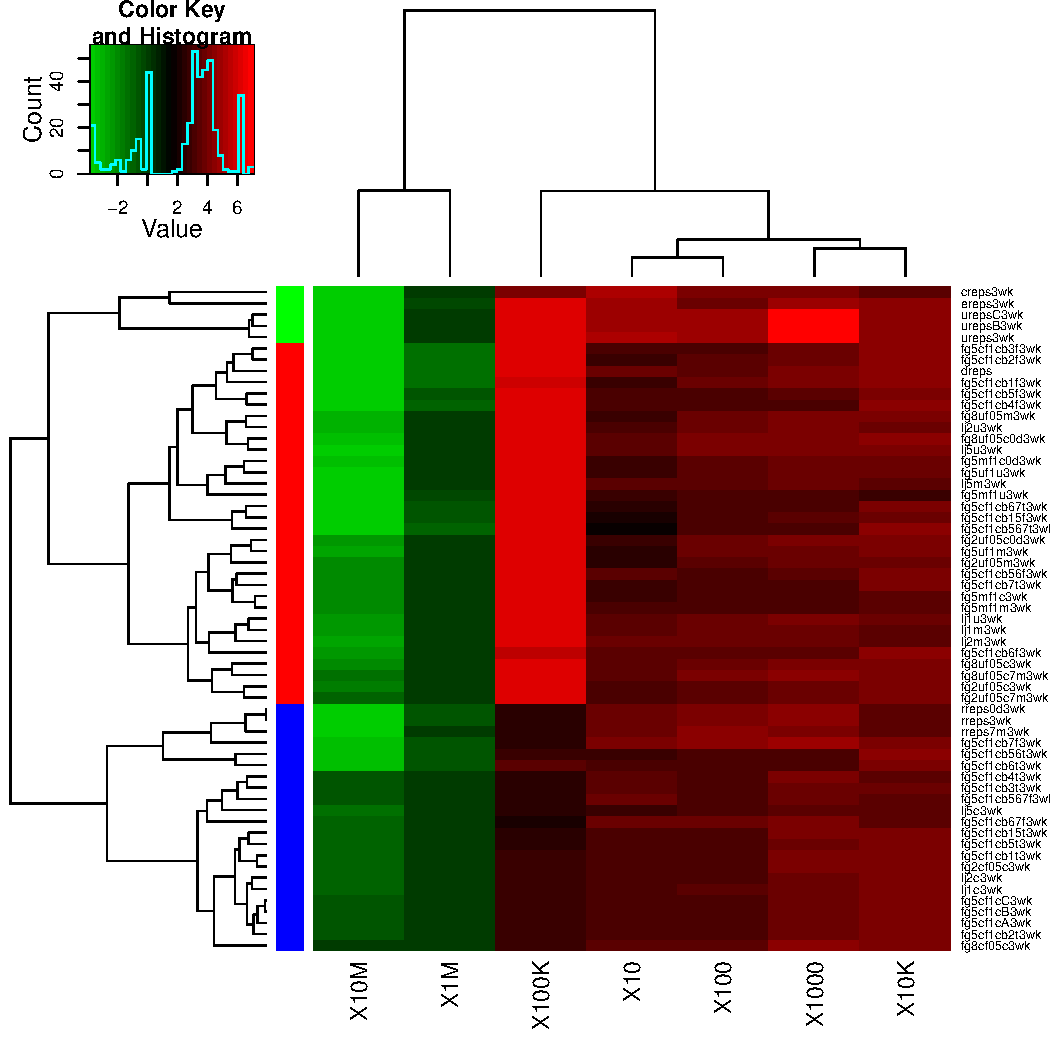
\includegraphics{figures/heatmap-sbucks-ments-star-med-medians-3wk}
    \caption{Starranks by mentions for all simulations seeded by 3 weeks of reality.}
    \label{figure:heatmap-sbucks-ments-star-med-medians-3wk}
\end{center}
\end{figure}
\pagebreak \subsubsection{Starranks for Replies}
\label{starranksforreplies}

We cluster median starranks per bucket, aggregated as overall medians for all days of each simulation, by distance from each other and {\itshape dreps}, the reality.  We segment the simulations by the amount of reality used to seed them, into four overall classes -- 0, 1wk, 2wk, and 3wk.


The initial generation places two non-bucketed simulations around {\itshape dreps}:


\begin{itemize}


\item fg5uf1u

\item fg5mf1u
\end{itemize}


\begin{figure}
\begin{center}
    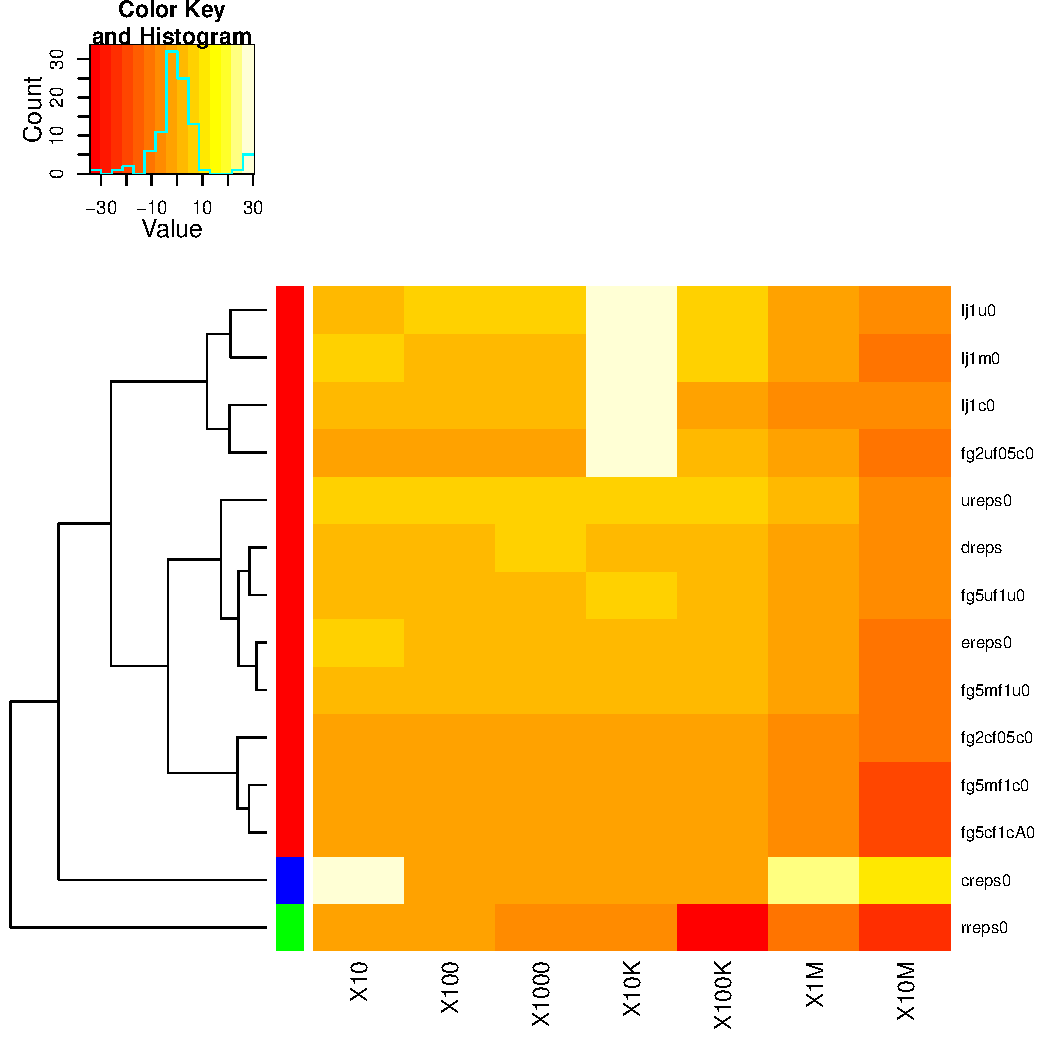
\includegraphics{figures/heatmap-sbucks-reps-star-med-medians-0wk}
    \caption{Starranks by replies for all simulations started from scratch.}
    \label{figure:heatmap-sbucks-reps-star-med-medians-0wk}
\end{center}
\end{figure}
In the first weeks, the simulated middle class {\itshape 6f} is already near reality.
Notable non-bucketed in the reality cluster are


\begin{itemize}


\item fg5uf1u

\item lj2m

\item fg5m1u
\end{itemize}


\begin{figure}
\begin{center}
    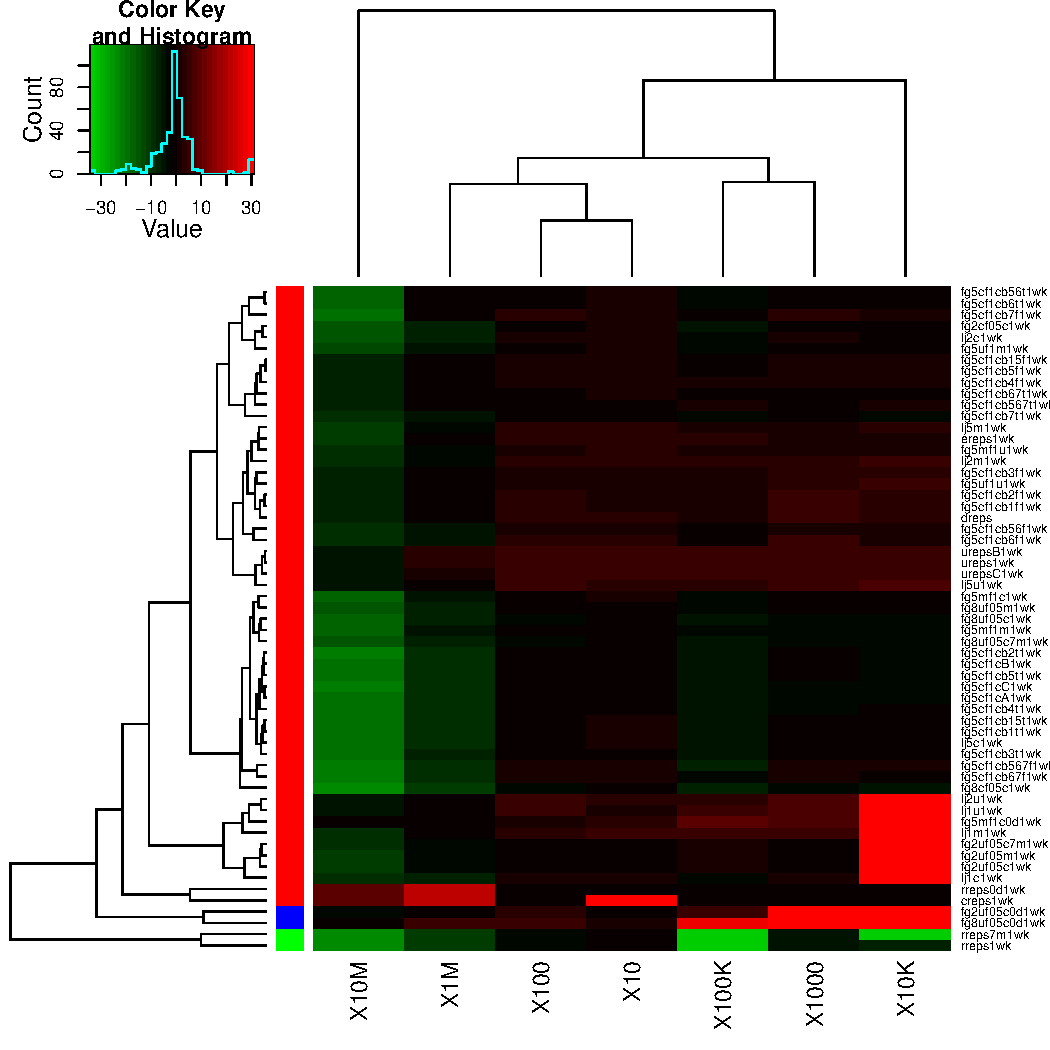
\includegraphics{figures/heatmap-sbucks-reps-star-med-medians-1wk}
    \caption{Starranks by replies for all simulations seeded by 1 week of reality.}
    \label{figure:heatmap-sbucks-reps-star-med-medians-1wk}
\end{center}
\end{figure}
The same picture, and the same wide range, of starranks by mentions persists after week 2 of reality.  The middle class {\itshape 6f} is right there, after {\itshape {1,2}f}, and our non-bucketed stay near:


\begin{itemize}


\item fg5uf1u

\item ereps

\item lj5m

\item fg5mf1u

\item fg8uf05c0d
\end{itemize}


\begin{figure}
\begin{center}
    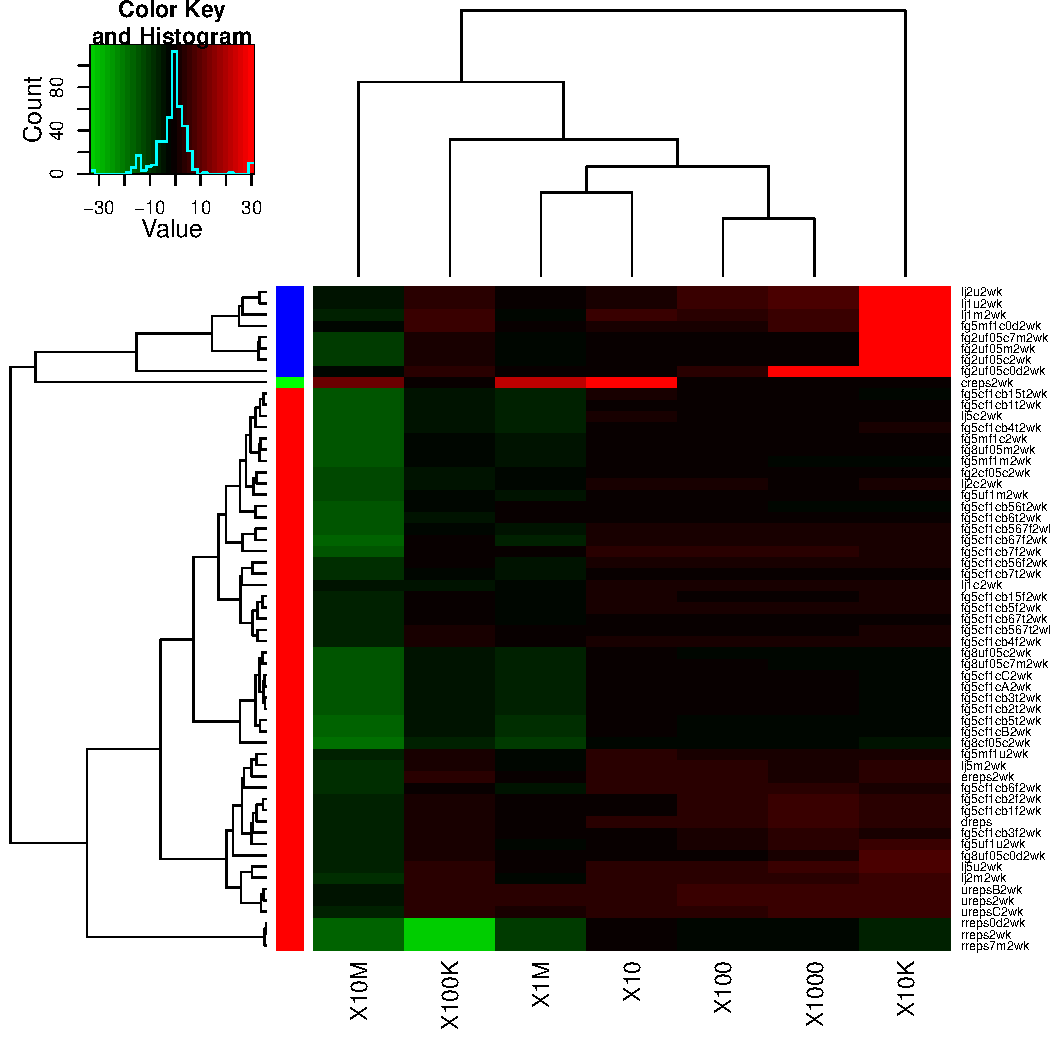
\includegraphics{figures/heatmap-sbucks-reps-star-med-medians-2wk}
    \caption{Starranks by replies for all simulations seeded by 2 weeks of reality.}
    \label{figure:heatmap-sbucks-reps-star-med-medians-2wk}
\end{center}
\end{figure}
Finally, in the third week, the exponent range of the starrank by mentions shrinks from [-30,30] to [-6,6], with the elite being all positive, dominating their audiences.


Zero-maturity capital-uniform non-bucketed simulations surround {\itshape dreps}now, with a FOF-uniform global uniform one from before, as well as utility, no-FOF, global uniforms:


\begin{itemize}


\item fg8uf05c0d

\item fg2uf05c0d

\item fg5mf1c0d

\item fg5uf1u

\item lj{1,2,5}m
\end{itemize}


\begin{figure}
\begin{center}
    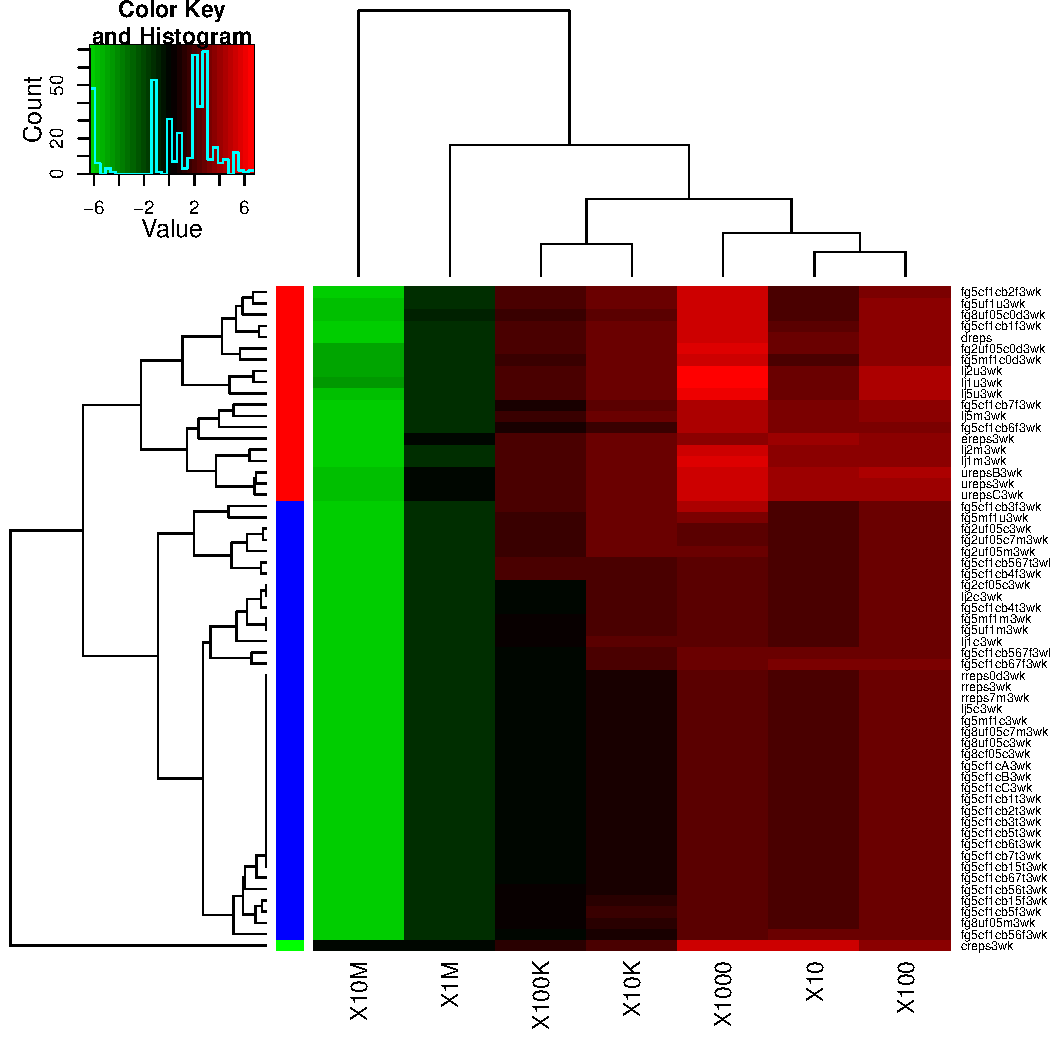
\includegraphics{figures/heatmap-sbucks-reps-star-med-medians-3wk}
    \caption{Starranks by replies for all simulations seeded by 3 weeks of reality.}
    \label{figure:heatmap-sbucks-reps-star-med-medians-3wk}
\end{center}
\end{figure}
\pagebreak \subsection{Bucket to Bucket Communication}
\label{buckettobucketcommunication}

\subsubsection{B2B Replies}
\label{b2breplies}

Communication to the higher-class buckets proceeds as follows.


When we generate from scratch --- Figure~\ref{figure:heatmap-b2br-befr-rel-medians-0wk}, --- global-uniform strategies fall closer to reality at first, such as


\begin{itemize}


\item fg5uf1u

\item lj{1,2,5}u

\item ereps

\item fg5mf1u
\end{itemize}

The first week --- Figure~\ref{figure:heatmap-b2br-befr-rel-medians-1wk}, ---  bucketed join, with small elite changes {\itshape {1,2,3}f} but also the simulated poor, {\itshape 7f} clustering around it.  Among the non-bucketed, neighbors include FOF mentions-uniform, with global mentions-uniform strategies.


\begin{itemize}


\item fg5uf1u

\item lj{1,2,5}u

\item ereps

\item fg5mf1u

\item lj{1,2,5}m
\end{itemize}

The second week --- Figure~\ref{figure:heatmap-b2br-befr-rel-medians-2wk}, ---  besides the simulated elites, we get the upper-middle class, separately and with the celebrities, still the same non-bucketed favorites:


\begin{itemize}


\item fg5cf1cb15f

\item fg5cf1cb5f

\item fg5uf1u

\item lj{1,2,5}u

\item ereps

\item fg5mf1u

\item lj{1,2,5}m

\item fg8uf05c0d

\item fg2uf05c0d
\end{itemize}

Finally, the third week --- Figure~\ref{figure:heatmap-b2br-befr-rel-medians-3wk}, ---  shows homogeneity across simulations, with the small simulated elites surrounding reality, and also


\begin{itemize}


\item lj{1,2,5}u

\item fg5cf1cb15f

\item fg5cf1cb5f

\item fg5uf1u

\item ereps
\end{itemize}


\begin{figure}
\begin{center}
    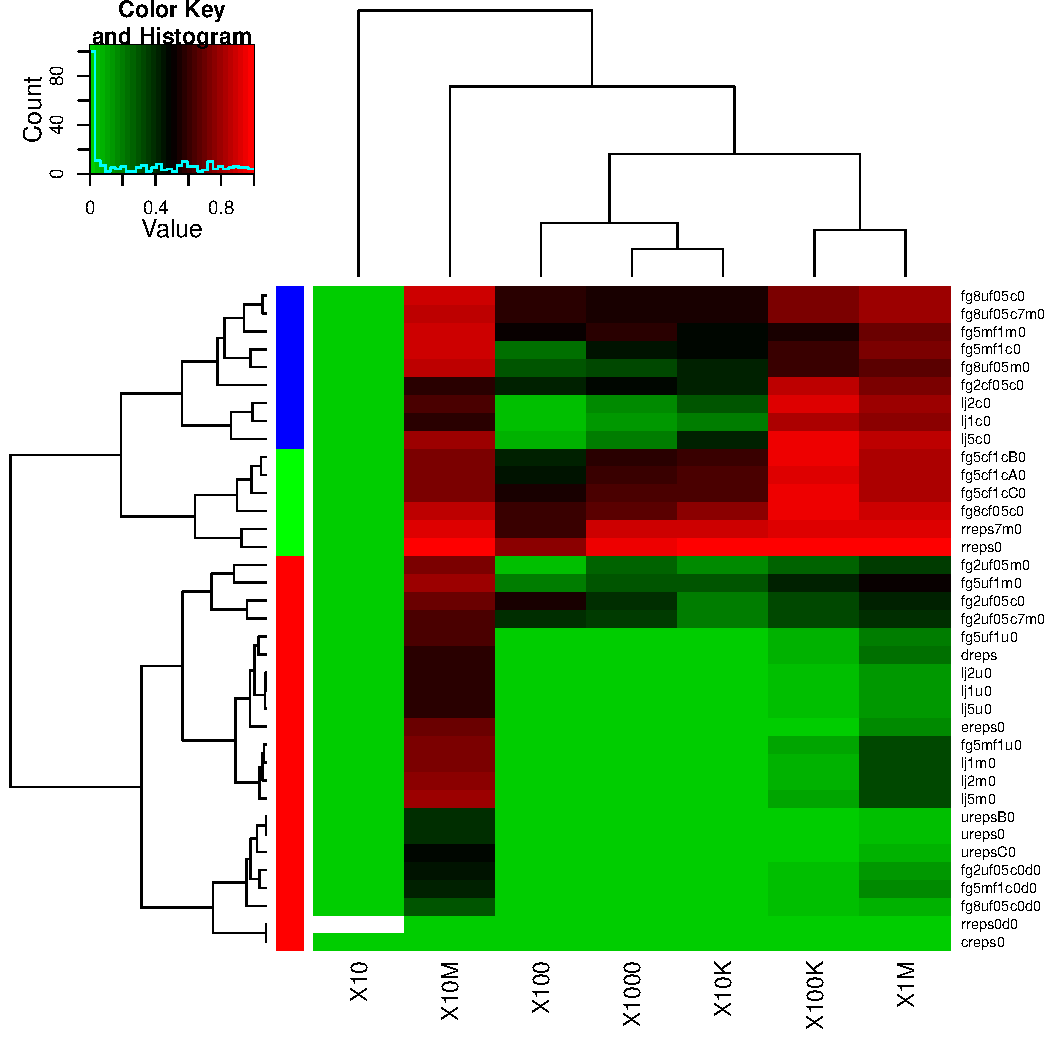
\includegraphics{figures/heatmap-b2br-befr-rel-medians-0wk}
    \caption{The fraction of all replies to higher buckets for all simulations started from scratch.}
    \label{figure:heatmap-b2br-befr-rel-medians-0wk}
\end{center}
\end{figure}

\begin{figure}
\begin{center}
    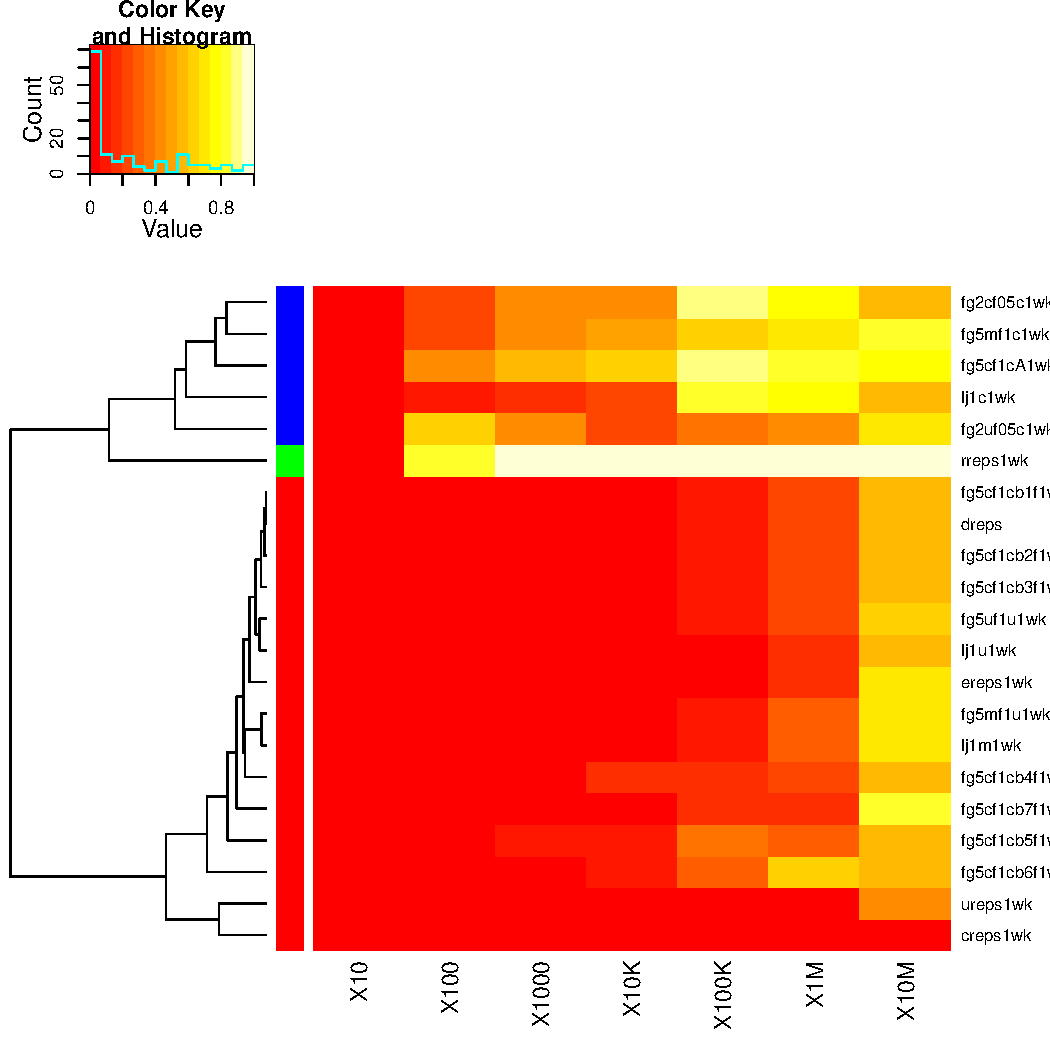
\includegraphics{figures/heatmap-b2br-befr-rel-medians-1wk}
    \caption{The fraction of all replies to higher buckets for all simulations seeded by 1 week of reality.}
    \label{figure:heatmap-b2br-befr-rel-medians-1wk}
\end{center}
\end{figure}

\begin{figure}
\begin{center}
    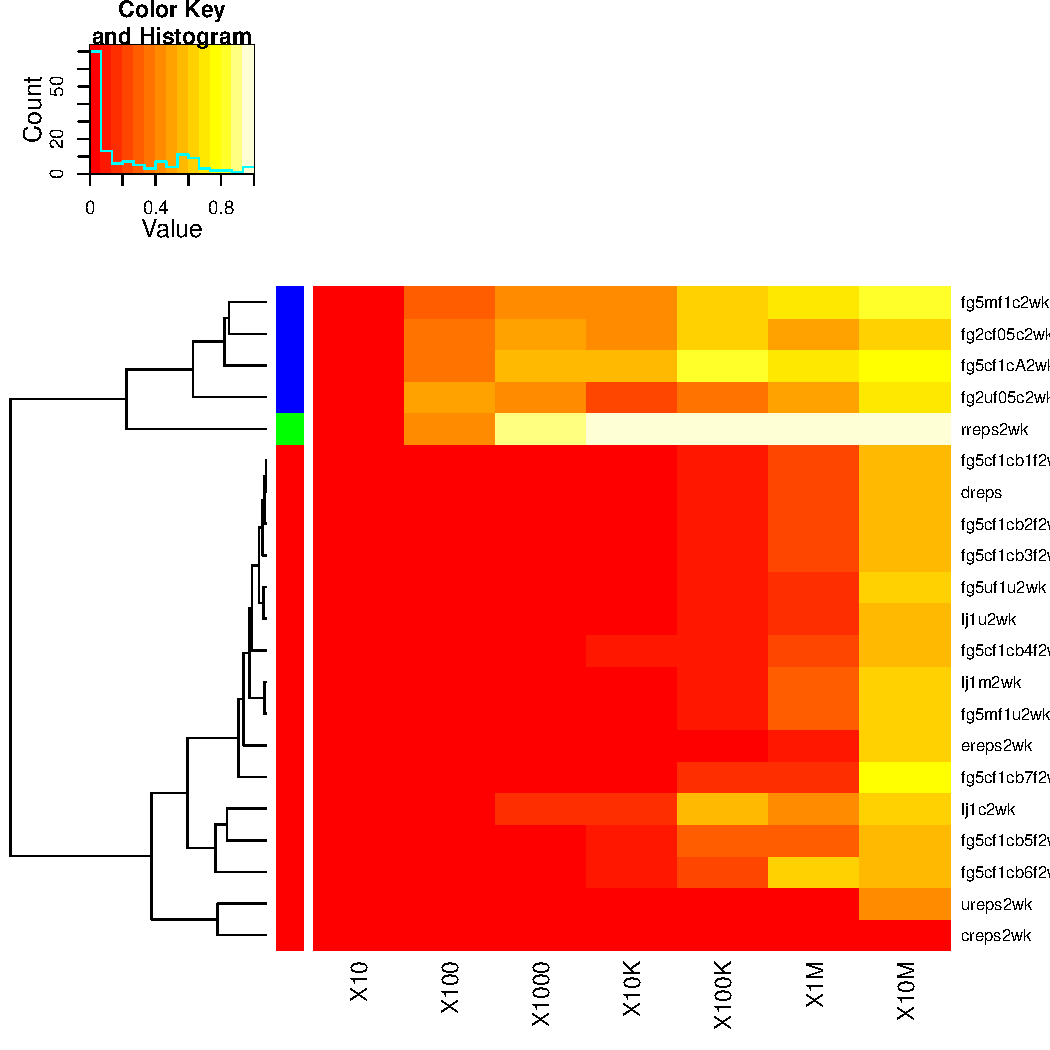
\includegraphics{figures/heatmap-b2br-befr-rel-medians-2wk}
    \caption{The fraction of all replies to higher buckets for all simulations seeded by 2 weeks of reality.}
    \label{figure:heatmap-b2br-befr-rel-medians-2wk}
\end{center}
\end{figure}

\begin{figure}
\begin{center}
    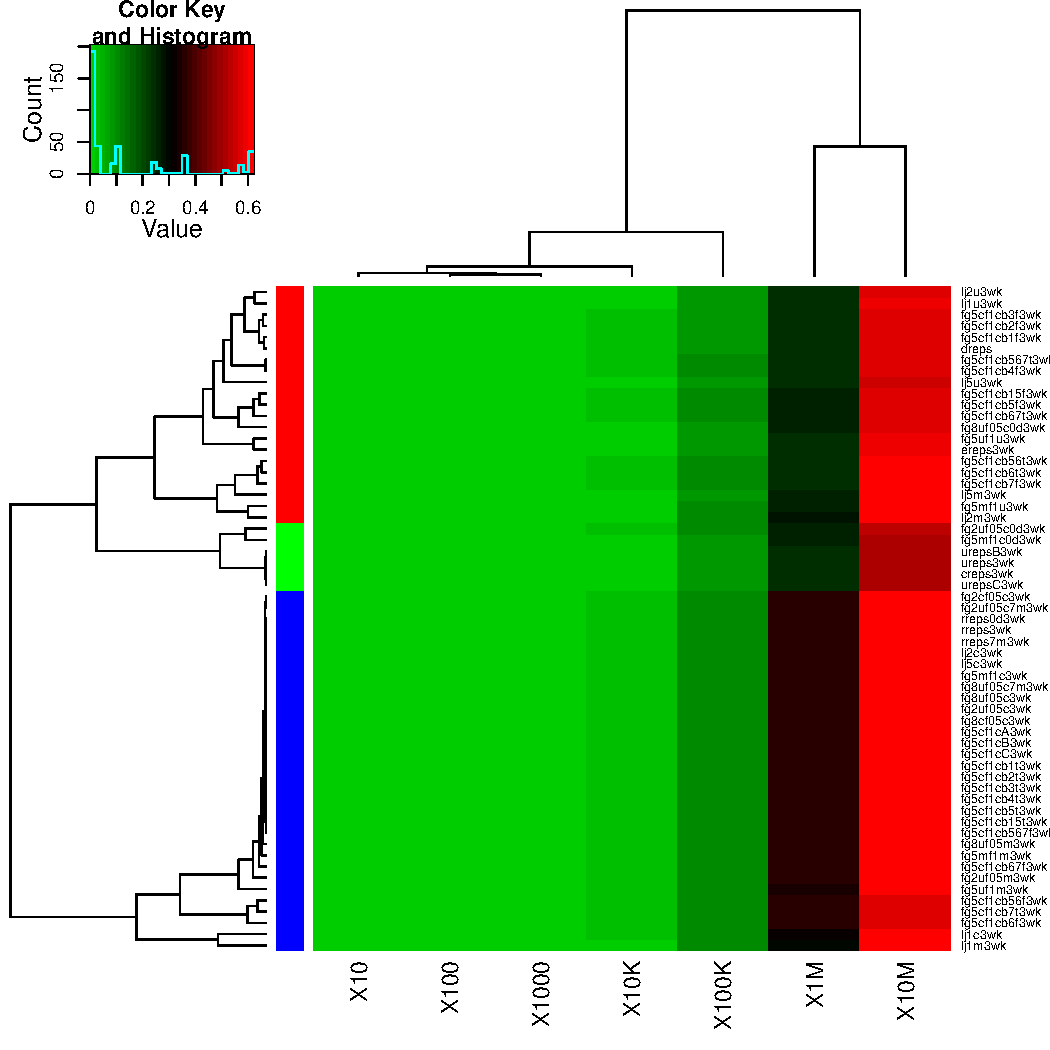
\includegraphics{figures/heatmap-b2br-befr-rel-medians-3wk}
    \caption{The fraction of all replies to higher buckets for all simulations seeded by 3 weeks of reality.}
    \label{figure:heatmap-b2br-befr-rel-medians-3wk}
\end{center}
\end{figure}
Communication with the lower-class buckets unfolds in the following way.


Straight out of the gate --- Figure~\ref{figure:heatmap-b2br-aftr-rel-medians-0wk}, --- utility-based strategies, with global uniform or mentions, and also 0.5 probability of FOF uniform mix, show up near the {\itshape dreps} reality:


\begin{itemize}


\item fg5uf1u

\item fg5mf1u

\item lj{1,2,5}m

\item ereps
\end{itemize}

With first week of reality seeded as the starting conditions --- Figure~\ref{figure:heatmap-b2br-aftr-rel-medians-1wk}, --- we see bucketed simulations, and also higher ratios of talking down from the elite buckets.  Small elites and the same winners as above are the closest to reality.   Capital-based simulations cluster together, both bucketed and not, as we bucket the same base, {\itshape fg5cf1c}.


The second week --- Figure~\ref{figure:heatmap-b2br-aftr-rel-medians-2wk}, --- we see the same pattern, with a few more global uniform combinations of FOF and pure utility:


\begin{itemize}


\item lj{1,2,5}u

\item fg8uf05c0d

\item fg5mf1c0d
\end{itemize}

Finally, the third week --- Figure~\ref{figure:heatmap-b2br-aftr-rel-medians-3wk} --- is fairly homogeneous and continues the evolving patterns, with the winners being small simulated elites and


\begin{itemize}


\item fg2uf05c0d

\item fg5uf1u

\item lj1u

\item fg5mf1u

\item lj{1,2}m
\end{itemize}


\begin{figure}
\begin{center}
    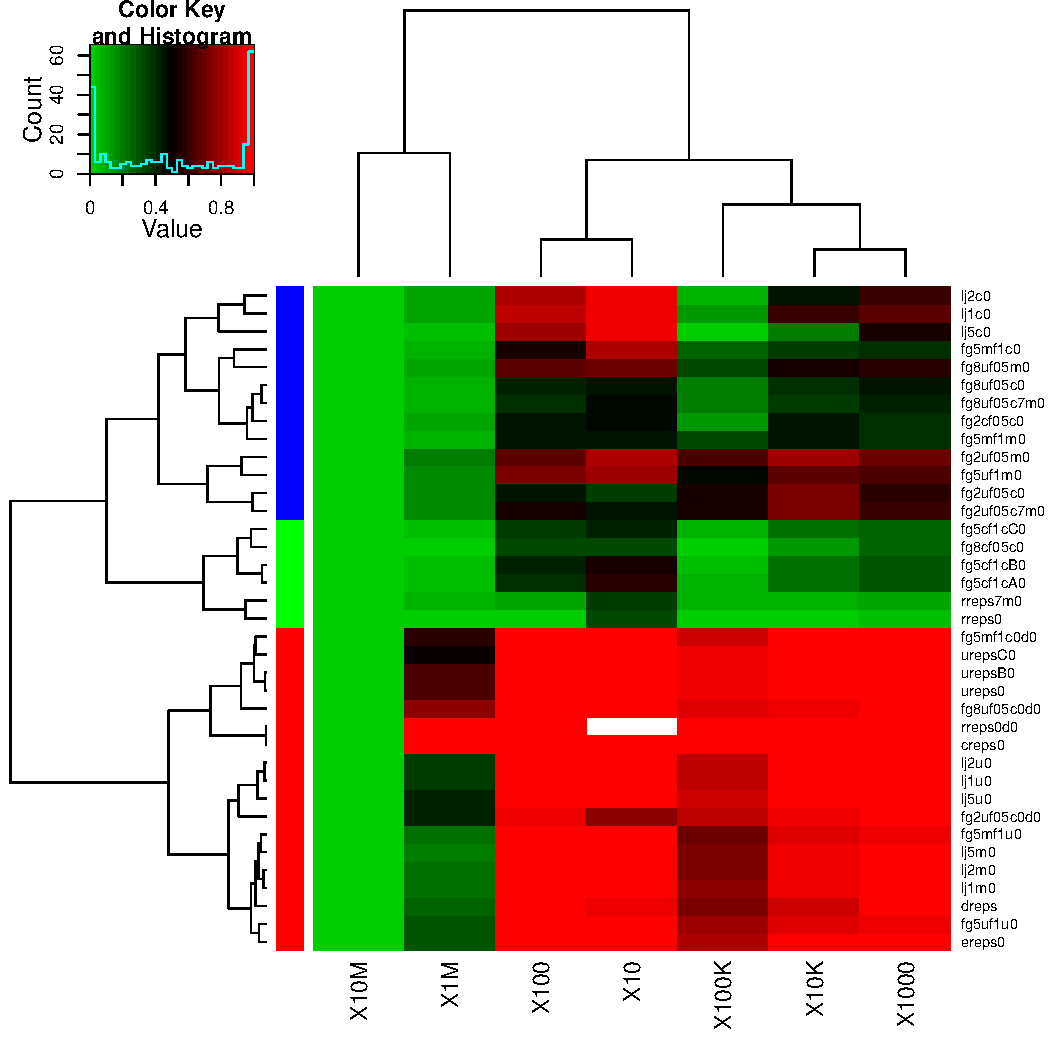
\includegraphics{figures/heatmap-b2br-aftr-rel-medians-0wk}
    \caption{The fraction of all replies to lower buckets for all simulations started from scratch.}
    \label{figure:heatmap-b2br-aftr-rel-medians-0wk}
\end{center}
\end{figure}

\begin{figure}
\begin{center}
    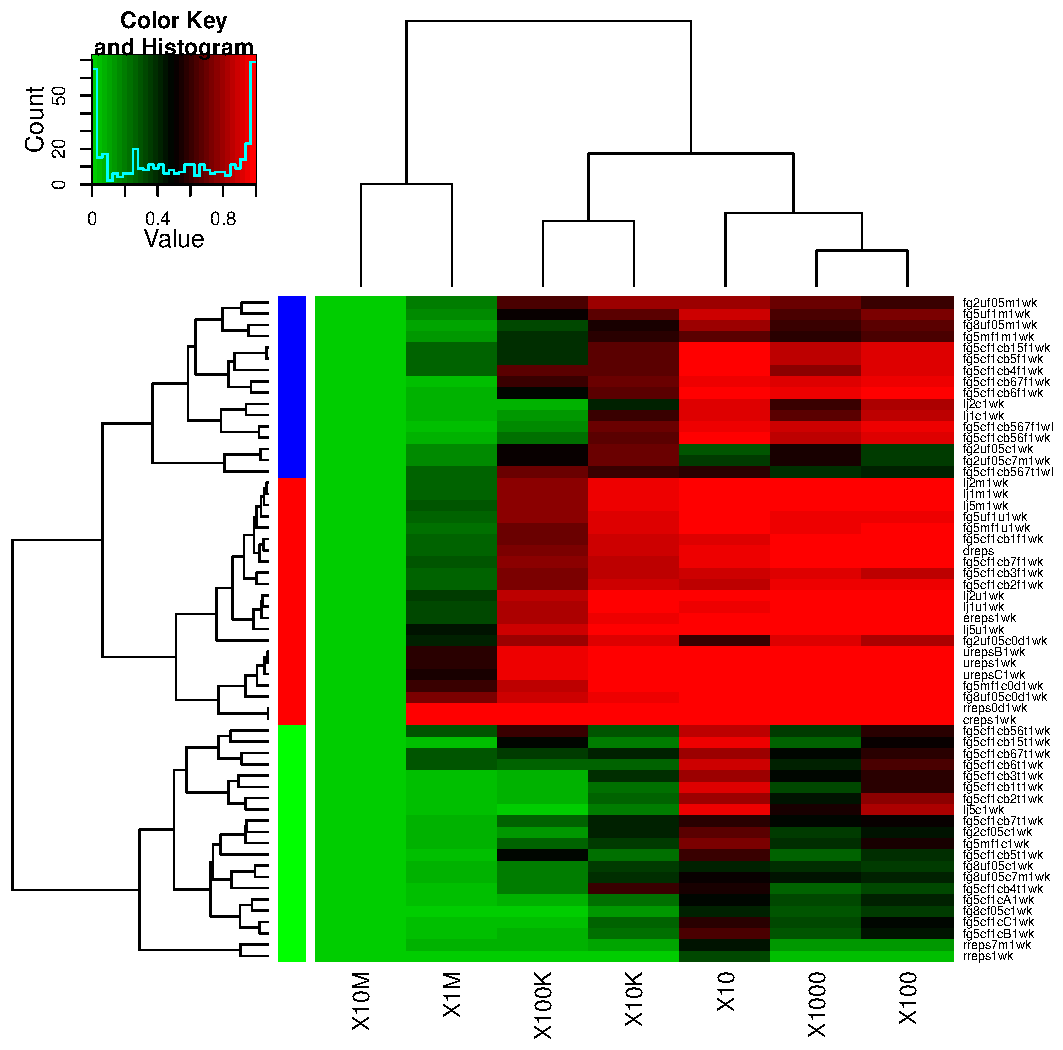
\includegraphics{figures/heatmap-b2br-aftr-rel-medians-1wk}
    \caption{The fraction of all replies to lower buckets for all simulations seeded by 1 week of reality.}
    \label{figure:heatmap-b2br-aftr-rel-medians-1wk}
\end{center}
\end{figure}

\begin{figure}
\begin{center}
    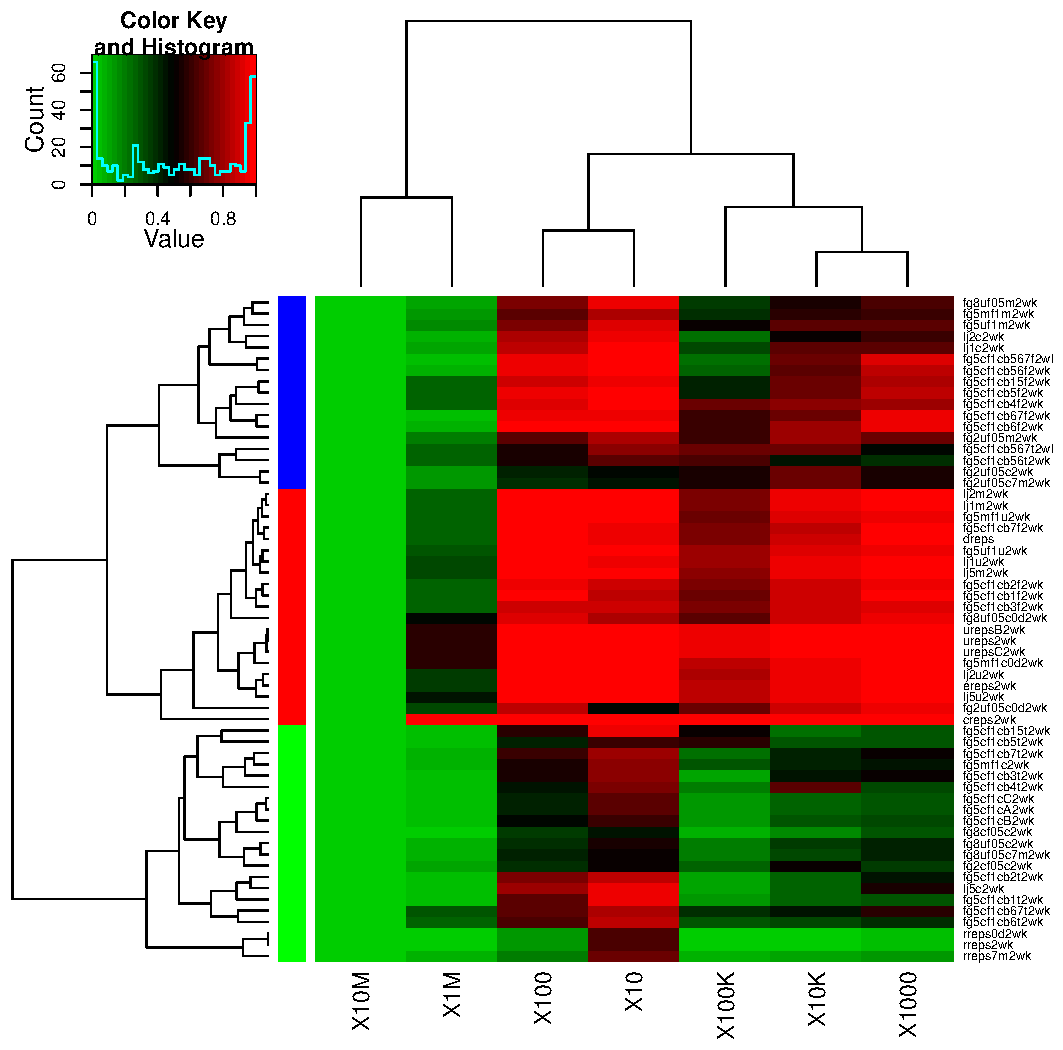
\includegraphics{figures/heatmap-b2br-aftr-rel-medians-2wk}
    \caption{The fraction of all replies to lower buckets for all simulations seeded by 2 weeks of reality.}
    \label{figure:heatmap-b2br-aftr-rel-medians-2wk}
\end{center}
\end{figure}

\begin{figure}
\begin{center}
    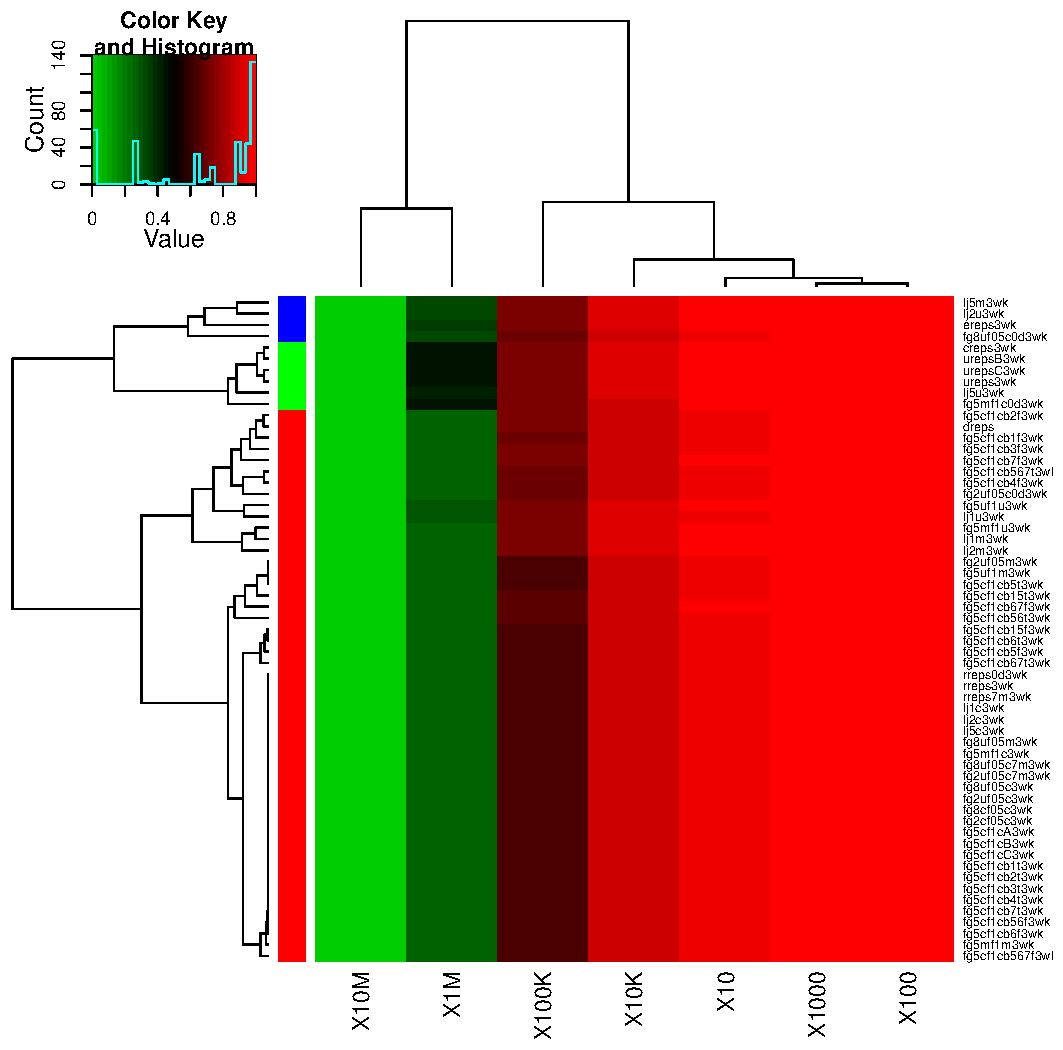
\includegraphics{figures/heatmap-b2br-aftr-rel-medians-3wk}
    \caption{The fraction of all replies to lower buckets for all simulations seeded by 3 weeks of reality.}
    \label{figure:heatmap-b2br-aftr-rel-medians-3wk}
\end{center}
\end{figure}
Communications which stay within the same bucket, for each bucket, develop as follows, with the ratios of all replies allocated to each bucket counted.


When simulating from scratch --- Figure~\ref{figure:heatmap-b2br-self-rel-medians-0wk}, --- we get our by now usual group of winners:


\begin{itemize}


\item fg5uf1u

\item fg5mf1u

\item lj{1,2,5}m

\item ereps




\item fg8uf05m




\item lj{1,2,5}c
\end{itemize}

The first week --- Figure~\ref{figure:heatmap-b2br-self-rel-medians-1wk} ---  adds the bucketed simulations, but they don't surround the reality just yet!  Our winners remain as above, with the small elites joined nearby by the simulated poor, and the simulated celebrity and upper-middle class combo, followed by just the latter:


\begin{itemize}


\item fg5cf1cb7f

\item fg5cf1cb15f

\item fg5cf1cb5f
\end{itemize}

The same winners persist through the second week --- Figure~\ref{figure:heatmap-b2br-self-rel-medians-2wk} ---  to the third --- Figure~\ref{figure:heatmap-b2br-self-rel-medians-3wk}, ---  when they are joined by the ebullient simulated middle class and immature capital-uniform FOF:


\begin{itemize}


\item fg5cf1cb6f

\item fg8uf05c0d
\end{itemize}


\begin{figure}
\begin{center}
    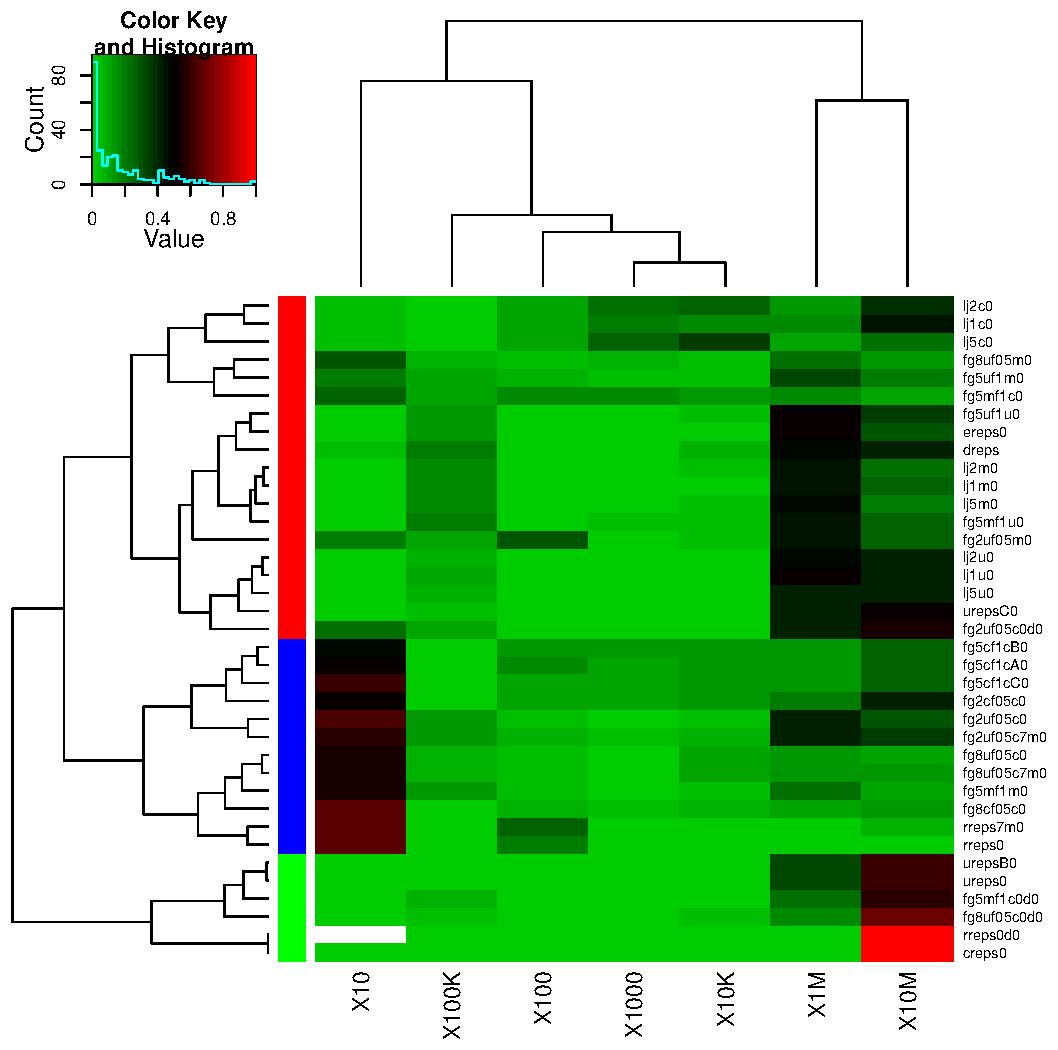
\includegraphics{figures/heatmap-b2br-self-rel-medians-0wk}
    \caption{The fraction of all replies to the same bucket for all simulations started from scratch.}
    \label{figure:heatmap-b2br-self-rel-medians-0wk}
\end{center}
\end{figure}

\begin{figure}
\begin{center}
    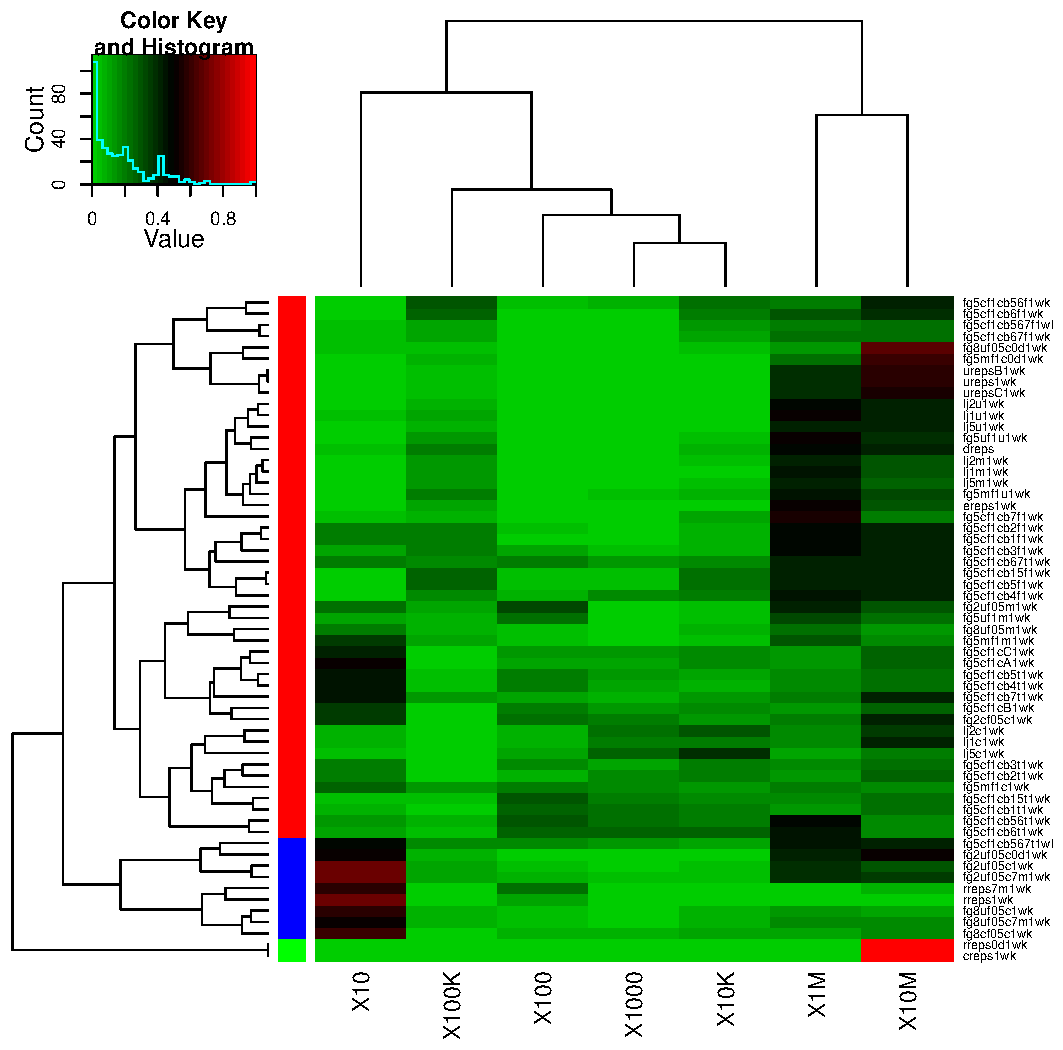
\includegraphics{figures/heatmap-b2br-self-rel-medians-1wk}
    \caption{The fraction of all replies to the same bucket for all simulations seeded by 1 week of reality.}
    \label{figure:heatmap-b2br-self-rel-medians-1wk}
\end{center}
\end{figure}

\begin{figure}
\begin{center}
    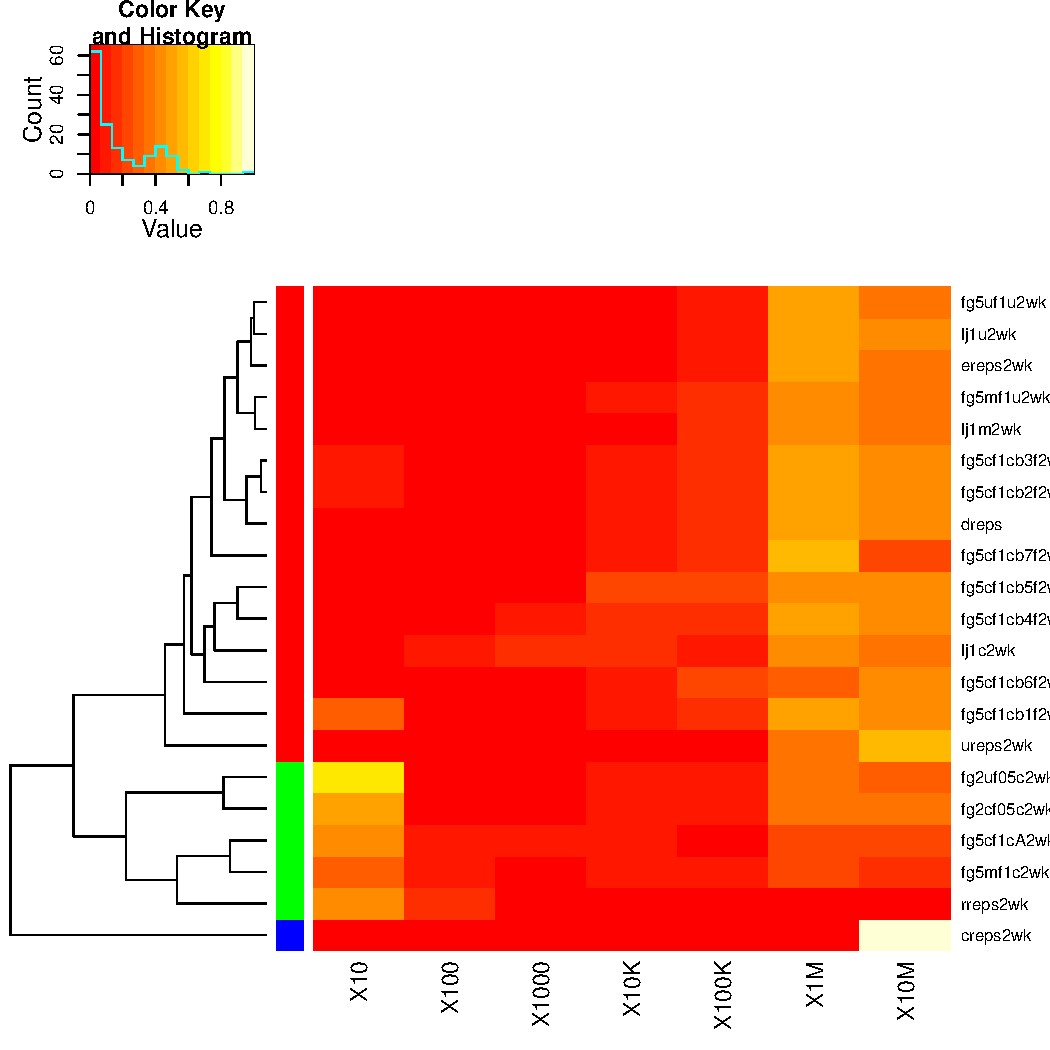
\includegraphics{figures/heatmap-b2br-self-rel-medians-2wk}
    \caption{The fraction of all replies to the same bucket for all simulations seeded by 2 weeks of reality.}
    \label{figure:heatmap-b2br-self-rel-medians-2wk}
\end{center}
\end{figure}

\begin{figure}
\begin{center}
    \includegraphics{figures/heatmap-b2br-self-rel-medians-3wk}
    \caption{The fraction of all replies to the same bucket for all simulations seeded by 3 weeks of reality.}
    \label{figure:heatmap-b2br-self-rel-medians-3wk}
\end{center}
\end{figure}
\pagebreak \subsubsection{B2B Mentions}
\label{b2bmentions}

Since bucket to bucket mentions from the higher classes are few, and decrease proportionally to the target bucket size, we do a $\log$ transform on the ratios.


When generating from scratch --- Figure~\ref{figure:heatmap-b2bm-befr-rel-medians-0wk} --- we get somewhat different set of nearest neighbors than for replies:


\begin{itemize}


\item fg5mf1u

\item fg5mf1c

\item fg5mf1m

\item fg8uf05m

\item fg5mf1c0d
\end{itemize}

The first week --- Figure~\ref{figure:heatmap-b2bm-befr-rel-medians-1wk} ---   brings the simulated middle class right next to reality.  The capital-based block is nearby.


The second week --- Figure~\ref{figure:heatmap-b2bm-befr-rel-medians-2wk} ---  keeps the middle class next to {\itshape dreps}, as well as the following:


\begin{itemize}


\item fg8uf05m

\item fg5uf1m

\item fg5cf1cb67f

\item fg5cf1cb7f

\item fg5cf1cb567f
\end{itemize}

Finally, by the third week --- Figure~\ref{figure:heatmap-b2bm-befr-rel-medians-3wk}, ---  the middle class is still the closest winner, among these ones:


\begin{itemize}


\item fg5cf1cb6f

\item fg2uf05c

\item fg8cf05c

\item fg5cf1cb56f

\item rreps

\item rreps0d
\end{itemize}


\begin{figure}
\begin{center}
    \includegraphics{figures/heatmap-b2bm-befr-rel-medians-log10-0wk}
    \caption{The fraction of all mentions from higher buckets for all simulations started from scratch.}
    \label{figure:heatmap-b2bm-befr-rel-medians-0wk}
\end{center}
\end{figure}

\begin{figure}
\begin{center}
    \includegraphics{figures/heatmap-b2bm-befr-rel-medians-log10-1wk}
    \caption{The fraction of all mentions from higher buckets for all simulations seeded by 1 week of reality.}
    \label{figure:heatmap-b2bm-befr-rel-medians-1wk}
\end{center}
\end{figure}

\begin{figure}
\begin{center}
    \includegraphics{figures/heatmap-b2bm-befr-rel-medians-log10-2wk}
    \caption{The fraction of all mentions from higher buckets for all simulations seeded by 2 weeks of reality.}
    \label{figure:heatmap-b2bm-befr-rel-medians-2wk}
\end{center}
\end{figure}

\begin{figure}
\begin{center}
    \includegraphics{figures/heatmap-b2bm-befr-rel-medians-log10-3wk}
    \caption{The fraction of all mentions from higher buckets for all simulations seeded by 3 weeks of reality.}
    \label{figure:heatmap-b2bm-befr-rel-medians-3wk}
\end{center}
\end{figure}
The pattern is really uniform here, every bucket is mentioned by its predecessors similarly, so we're only showing the typical values.  The bar plot in Figure~\ref{figure:b2bm-aftr-rel-medians-med} shows the values per bucket of the fraction of all mentions this bucket received from lower classes, aggregated as medians for bucket classes across all simulations.



\begin{figure}
\begin{center}
    \includegraphics[width=4in]{figures/b2bm-aftr-rel-medians-med}
    \caption{Medians of all bucket to bucket mentions, from lower ones than each one, for all simulations seeded by 3 weeks of reality, per bucket.}
    \label{figure:b2bm-aftr-rel-medians-med}
\end{center}
\end{figure}
The fraction of mentions, staying in the same bucket, progresses as follows.


From scratch --- Figure~\ref{figure:heatmap-b2bm-self-rel-medians-0wk}, --- the cluster neighbor of reality is


\begin{itemize}


\item fg2uf05m
\end{itemize}

The first week --- Figure~\ref{figure:heatmap-b2bm-self-rel-medians-1wk}, --- the winners are


\begin{itemize}


\item lj5c1

\item fg5cf1cb7t

\item fg5uf1m

\item fg5cf1cb7f

\item fg8uf05m

\item fg5cf1cb567f

\item fg5cf1cb67f
\end{itemize}

The second week --- Figure~\ref{figure:heatmap-b2bm-self-rel-medians-2wk}, --- the near neighbors of {\itshape dreps} are


\begin{itemize}


\item fg2cf05c

\item lj1c2

\item fg2uf05c0d

\item fg8uf05m
\end{itemize}

The third week --- Figure~\ref{figure:heatmap-b2bm-self-rel-medians-3wk}, --- these simulations are in proximity to {\itshape dreps}:


\begin{itemize}


\item fg2uf05m

\item fg5cf1cb2f

\item fg5cf1cb15f

\item fg5cf1cb67t

\item dreps

\item urepsB

\item ureps3

\item fg2cf05c
\end{itemize}


\begin{figure}
\begin{center}
    \includegraphics{figures/heatmap-b2bm-self-rel-medians-log10-0wk}
    \caption{The fraction of all mentions from the same bucket for all simulations started from scratch.}
    \label{figure:heatmap-b2bm-self-rel-medians-0wk}
\end{center}
\end{figure}

\begin{figure}
\begin{center}
    \includegraphics{figures/heatmap-b2bm-self-rel-medians-log10-1wk}
    \caption{The fraction of all mentions from the same bucket for all simulations seeded by 1 week of reality.}
    \label{figure:heatmap-b2bm-self-rel-medians-1wk}
\end{center}
\end{figure}

\begin{figure}
\begin{center}
    \includegraphics{figures/heatmap-b2bm-self-rel-medians-log10-2wk}
    \caption{The fraction of all mentions from the same bucket for all simulations seeded by 2 weeks of reality.}
    \label{figure:heatmap-b2bm-self-rel-medians-2wk}
\end{center}
\end{figure}

\begin{figure}
\begin{center}
    \includegraphics{figures/heatmap-b2bm-self-rel-medians-log10-3wk}
    \caption{The fraction of all mentions from the same bucket for all simulations seeded by 3 weeks of reality.}
    \label{figure:heatmap-b2bm-self-rel-medians-3wk}
\end{center}
\end{figure}
\pagebreak \subsection{Skew Correlation}
\label{skewcorrelation}

We look at $\tau$ alignment for the full lists of all users and their capitals and skews for each day, and also do it per bucket. 
For most of our strategies, we observe a Kendall's $\tau$ correlation between social capial and skew of about 0.2.  It reaches 0.3 for {\itshape fg5m1u}, and is lower for {\itshape fg5c1cA} (and B,C) seeded with two or less weeks.
The fact that the global $\tau$ generally is around 0.2, as it is for {\itshape dreps}, shows that politician-like behavior, with more communication activity toward the top contributors, corresponds to the social capital hierarchy.


From scratch, --- Figure~\ref{figure:heatmap-cstau-0wk} we observe a significant amount of low correlations among the global-only simulations, and a progressive drops for capital-capital ones.  FOF-based simulations with 0.05 jumpFOF probability and global uniform strategy stay nearest the reality.


One week of reality seeding --- Figure~\ref{figure:heatmap-cstau-1wk} --- brings about the bucketed simulations, which cluster around {\itshape dreps}, as expected, starting with small elite buckets.  Interesting early neighbors are


\begin{itemize}


\item lj1u

\item fg5mf1c
\end{itemize}

-- followed by a block of the original capital-uniform ones with large FOF probability (i.e.\ low 0.05 jumpFOF probability of going global away from FOF).


Capital-capital simulations, together with {\itshape rreps} and {\itshape creps}, are in a more distant cluster, falling rapidly with time.


The simulated middle class, {\itshape fg5cf1cb6f}, ends up in a separate cluster with
* lj{2,5}u
* lj{1,2,5}m
* fg5uf1{m,u}
* fg5mf1{c0d,u}


They fall a bit slower than {\itshape dreps}, as opposed to capital-capital ones.


The picture consolidates after two weeks of reality --- Figure~\ref{figure:heatmap-cstau-2wk} --- with a large cluster around {\itshape dreps}.  Now we see simulated middle classes and elites, {\itshape fg5cf1cb7t}, as well as the simulated poor, {\itshape fg5cf1cb7f}, next to each other and near {\itshape dreps} -- meaning that the middle class is approximated quite well by the capital-capital strategy in relation to the poor.  


The middle class, simulated by itself, {\itshape fg5cf1cb6f}, is between the previous favorites:


\begin{itemize}


\item fg5mf{1c0d,c}

\item lj{1,2}u

\item fg2uf05m

\item fg5uf1m

\item fg5cf1cb6f
\end{itemize}

Finally, after three weeks of reality, --- Figure~\ref{figure:heatmap-cstau-3wk} --- all but one non-bucketed capital-capital simuations get out of the distant cluster, now left to globals only --- {\itshape ureps}, {\itshape ereps}, {\itshape creps}, {\itshape rreps}, and {\itshape fg8cf05c}.


The preserved middle class by itself, {\itshape fg5cf1cb6t}, is closer to reality than simulated-only, {\itshape fg5cf1cb6f}, which is near the edge of the adjacent cluster, next to {\itshape fg5mf1u}.  FOF-based strategies with high probability of FOF attachment, 0.95,  and high probability of jumping away from the initial utility, 0.8, are the closest to reality after the bucketed elites, namely


\begin{itemize}


\item fg8uf05{m,c7m,c0d,c}
\end{itemize}

Among the bucketed simulations, nearest non-elite ones are


\begin{itemize}


\item fg5cf1cb15f

\item fg5cf1cb7t

\item fg5cf1cb56f
\end{itemize}

Simulating the middle and upper middle class, just two or with all the elites, with our capital-capital strategies turns out to be a good approximation of politician-like behavior, by skew.



\begin{figure}
\begin{center}
    \includegraphics[width=4in]{figures/kendall-tau-fg5mf1u0-fg5cf1c0}
    \caption{Global correlation of social capital and skew by Kendall $\tau$.  While generally staying around 0.2-0.3, it can also decrease for some strategies, like the all-capital one.}
    \label{figure:kendall-tau-fg5mf1u0-fg5cf1c0}
\end{center}
\end{figure}

\begin{figure}
\begin{center}
    \includegraphics{figures/heatmap-cstau-0wk}
    \caption{Kendall’s $\tau$ correlation between social capital and skew, all simulations started from scratch.}
    \label{figure:heatmap-cstau-0wk}
\end{center}
\end{figure}

\begin{figure}
\begin{center}
    \includegraphics{figures/heatmap-cstau-1wk}
    \caption{Kendall’s $\tau$ correlation between social capital and skew, all simulations seeded with one week of reality.}
    \label{figure:heatmap-cstau-1wk}
\end{center}
\end{figure}

\begin{figure}
\begin{center}
    \includegraphics{figures/heatmap-cstau-2wk}
    \caption{Kendall’s $\tau$ correlation between social capital and skew, all simulations seeded with two weeks of reality.}
    \label{figure:heatmap-cstau-2wk}
\end{center}
\end{figure}

\begin{figure}
\begin{center}
    \includegraphics{figures/heatmap-cstau-3wk}
    \caption{Kendall’s $\tau$ correlation between social capital and skew, all simulations seeded with three weeks of reality.}
    \label{figure:heatmap-cstau-3wk}
\end{center}
\end{figure}
\pagebreak \subsection{Discussion}
\label{discussion}

\label{section:discussion}
So, are the influentials accidental, or not, after all?


The staying rate within the same simulation shows how stable the winners are within their own classes -- if the churn in buckets is not too great, especially among the higher classes, we have our influentials which keep their positions for long periods of time, as they do in the real world.


What we see with the staying rates in simulations is this: the more elaborate a simulation is, the higher the staying rates are -- that is, the winners in a given world are not random, they persist from day to day.  Global uniform attachment doesn't achieve any staying power below celebrity level, and any combination with uniform attachment loses to those with mentions- or capital-based ones.  E.g., compare the staying power of {\itshape fg2uf05m}, {\itshape fg2uf05c}, and {\itshape fg2cf05c} or {\itshape fg5cf1c} in Figure~ref{figure:heatmap-srates-medians-2wk} -- capital-based global attachment significantly increases stability of the top buckets.


The uniform simulations, {\itshape ureps}, are very telling about what may be the nature of this -- they have almost no staying rate in any higher-class buckets, except for the very top -- where the celebrities are surprisingly persistent, with a staying rate of 60-70\% --- see  Figures~ref{figure:heatmap-srates-medians-1wk}--ref{figure:heatmap-srates-medians-2wk}.   However, a comparison between different runs of {\itshape ureps}, -- {\itshape ureps}, {\itshape urepsA}, and {\itshape urepsB} groups, -- shows that there's almost no overlap among the celebrities across the groups.  What happens in the uniform case is that almost everybody is dirt poor, with meaningless connections not rewarding them with any social capital.  However, somebody will get lucky merely by chance, in the beginning, and return a reply, achieving a reward.  Then, they will be likely to stay there, especially if they activity was high.


The capital-based attachments achieve a staying rate which is in some cases even higher than the real ones.  The uniform-based FOF and global simulations rank lower than the mention-based ones, and indeed, mentions are the key component of social capital.  The increase of the staying rates with increase in the intelligence of the behaviors used to attain them confirms that ``doing the right thing'' keeps the winners on top, proving they are not accidental under given conditions.


The overlap among the simulated winners and the real ones, while minimal, is not random.  It gets closer to 10\% per bucket of the upper middle classes for some of the elaborate, utility/FOF-capitalmention global-capital/mention simulations, such as {\itshape fg5mf1{m,c,c0d}} in Figure~\ref{figure:heatmap-overx-dreps-medians-3wk}.  Among the non-bucketed simulations, {\itshape lj1c} is doing quite well, capturing some of the 10K class winners.   It means that in a world with slightly different rules, other people will win -- if everybody attaches according to slightly different rules, those who were in a good starting position (seeded with {\itshape dreps}, show up on the same day), and are active enough (outdegree preserved), will fit better.


Among the same type of simulation, generated with different initializations of the random number generator, we get much higher overlap than with any other simulation.  It means that the classes we define are mostly held for the same type of strategy, i.e., the combination of the reciprocal social capital metric and class segmentation depends mostly on the behaviors themselves.


Thus our conclusion is that the influentials, defined with all the assumptions and ramifications of the underlying metric and class bucketing, are not accidental in their own worlds -- and hence probably the ones in our own world deserve the places they work hard to occupy, by most accounts.  The more intelligent they are, the better they stay on top, and grab a better share of the real-world winners in overlaps.  However, the top celebrities can be persistent even in a version of a stochastic world, and a slight change of rules will lead to a new and distinct persistent hierarchy which stays around under the same conditions, even though all of the edges are rearranged.  Seeding with the starting conditions from the real world doesn't lead to the real world hierarchy to continue, except for a few days immediately after the hand-off; but the new hierarchy is stable enough in smart simulations.


The fact that simulating elites does not change things as much as altering the upper middle class and on down tells us the elites do not define the communication structure as much as those primary classes.


Simulating the middle class or not is often not very different because it is in fact a fairly faithful simulation.  When fitting a linear model against all the buckets, determining the euclidian distance from reality --- 0 for reality itself --- we get buckets 4, 5 and 7, keeping which preserves it the most.  The top 3 elite buckets don't figure; the poor 7 dominates by its sheer bulk, while the upper middle class and the following ``upper crust'' bucket probably use strategies quite different from the capital-capital one we used.


We plotted distance of a function of preserving or simulating several bottom classes in Figures~\ref{figure:boxplot-x4}, \ref{figure:boxplot-x5}, \ref{figure:boxplot-x6}, \ref{figure:boxplot-x7}.  All but the middle class (bucket 6) figure as significant in a linear model on all features.  While preserving most classes brings the distance lower, the middle class is simulated well enough to make its preservation not significant, distance-wise.



\begin{figure}[ht]
\minipage[b]{0.5\linewidth}
\centering
\includegraphics[scale=0.4]{figures/boxplot-x4-cb}
\label{figure:boxplot-x4}
\caption{distance by the top 10K}
\endminipage\hfill%
%
\minipage[b]{0.5\linewidth}
\centering
\includegraphics[scale=0.4]{figures/boxplot-x5-cb}
\label{figure:boxplot-x5}
\caption{distance by the upper middle class}
\endminipage

\bigskip

\minipage[b]{0.5\linewidth}
\centering
\includegraphics[scale=0.4]{figures/boxplot-x6-cb}
\label{figure:boxplot-x6}
\caption{distance by middle class}
\endminipage\hfill%
%
\minipage[b]{0.5\linewidth}
\centering
\includegraphics[scale=0.4]{figures/boxplot-x7-cb}
\label{figure:boxplot-x7}
\caption{distance by the poor}
\endminipage
\end{figure}

Figure~\ref{figure:decision-tree-overx-dreps} shows a decision tree, fitting the distance for the overlap with reality (overx-dreps) from the ideal.  We use Euclidian distance for a 7-component vector corresponding to the class buckets.  We intentionally treat each bucket equally in this distance throughout our metrics, since preserving the actual hierarchy is important for the role of the elites, while any weighting by the bucket size would overwhelm them.


We see that the poor dominate by their volume, but then capital strategies work better, as well as using utility-based atatchment



\begin{figure}
\begin{center}
    \includegraphics{figures/decision-tree-overx-dreps}
    \caption{Decision tree on all features, fitting distance from reality.}
    \label{figure:decision-tree-overx-dreps}
\end{center}
\end{figure}
Bucket 4, the top 10K users by social capital after the preceding 1110, show the highest Kendall $\tau$ correlation with the skew measure of politician-like behavior we devised.  It means they are most attentive to the difference in input between their highest and lowest contributors, and most consistent in repaying those proportionally.  They, together with the upper middle class, bucket 5, also figure as significant in linear models and decision trees regressing the overlap with reality on preserving or simulating individual buckets.


The most important finding in our work is a persistent middle class, which is both defined and captured quite well by our reciprocal social capital.  As defined, the 1 M bucket above the poor, in the hierarchy segmented by that capital, the middle class is responsible for about 40\% of all outgoing replies overall (Figure~\ref{figure:vols4-re-norm-medians-med}).  It clusters near reality in most of the metrics, notably overlap with it, when replacing ``just'' the whole middle class with its simulation via {\itshape fg5cf1c} simulation -- attaching to FOFs and globally proportionally to social capital in the previous cycle, and using local utility optimization against the same capital.  


The fact that the middle class behaves consistently near reality in both true and capital-simulated form in most of our evaluations means that


\begin{itemize}


\item the middle class is working hard to keep the conversation going

\item it is trying to operate in a balanced, equitable manner

\item it has a high energy to produce a big share of all discourse

\item it is in no way random, regardless of the elites

\item it is responsible for many of the effects we care about in our measures

\item and hence is the real influencers we should care about, not those elites where randomness may depend on a point of view
\end{itemize}

\pagebreak \chapter{Data Mining Infrastructure}
\label{datamininginfrastructure}

\label{chapter:datamining-infrastructure}


\section{Importance of Social Programs}
\label{importanceofsocialprograms}

Any massive data mining of social networks has to overcome scaling problems and provide engineering solutions to the challenges which such amount of data poses.  We do not consider algorithmic part of the effort separate from programming -- on the contrary, we firmly believe that the way in which the ideas are formulated in computer science is inseparable from their effective implementation, which includes the lifecycle of a program as a materialized idea.  Efficiency includes not just the performance of a system, but also the ease of its coding, maintenance, understanding, and thus spreading and evolution.


Moreover, the modern social media community is driven by a dynamic class of cutting-edge hyperconnected geeks, who co-evolve the networking platforms and software environments enabling their programming, coding, scaling, and presentation.  This co-evolution started with PHP, skyrocketed with Ruby on Rails, and continues with modern {\itshape functional} languages, exceedingly via open-sourced, social coding.  In fact, the rise of the first social coding platform, \href{http://github.com}{github}\footnote{\href{http://github.com}{http://github.com}}, accelerated this process. Many day-to-day discussions among those building the social networks of today and tomorrow happen on Twitter.  Thus following the modern techniques, languages, and tools is key to advancing this revolution.  An example of the process is the Clojure programming language, pushing the envelope on abstraction, software engineering philosophy, new web paradigms, and social coding, which held its first ever conference, \href{http://clojure-conj.org/}{Clojure Conj}\footnote{\href{http://clojure-conj.org/}{http://clojure-conj.org/}} in October 2010.


In the spirit of the community, we make all of the code developed throughout this research open source and available on github under the Creative Commons license.


\pagebreak \section{Streaming API}
\label{streamingapi}

\label{StreamingAPI}


Gathering and storing Twitter data efficiently is a significant part of the job of analyzing it.  We've investigated several setups before arriving at our current one.  Previously, people used to crawl Twitter, calling the query API provided to get individual users' tweets.  The API has a rate limit for queries, but researchers can have their machines ``whitelisted,'' which actually just raises the limit quite high.  Twitter folks don't like anybody getting a hold of any significant fraction of all tweets, so any attempt to crawl aggressively often hit a permanent ban.  Since many people had a use for tweet streams, Twitter set up a separate Streaming API.  Instead of pulling information with SOAP queries from the web service, Streaming API is pushing a constant stream of tweets over an open HTML channel, which stays open.  There are several levels of streaming:


\begin{itemize}


\item The {\itshape firehose} being the full set of all tweets, pushed out in near real time.  {\itshape Firehose} is provided on a commercial basis to big players.  




\item The next level is {\itshape gardenhose}, which is, in Twitter's words, ``statistically representative'' of the firehose.  When we started gathering the gardenhose in mid-2009, we collected about 2 million tweets a day; a year later, we were getting more than 5 million tweets daily through it.  The {\itshape gardenhose} seems to be a round-robin sample of the latest tweets, and it does not provide a continuous coverage of any particular individual.  Nevertheless, we found that those who tweet a lot are represented proportionally in the gardenhose.




\item Another stream is called {\itshape shadow}, and allows to follow a set of users completely; our limit of shadowing is the maximum that research access allows, up to 50,000 people.  



\end{itemize}

When we started our studies, we computed the top pairs of repliers, chosen as follows.  For the replier graph, we looked at all pairs of users engaged in dialogues and having the most exchanges, then sorted them by the descending strength of the dialogues (computed as a function of the daily and total volume).  Then we took the top 50,000 of this ordered list.  It was interesting to see who was on top -- several couples, separated by distance, and also users engaged in explicit talk with several partners simultaneously.  Apparently they used Twitter as a sort of SMS service without realizing it's publicly available; most of them had closed their tweets from the public a few weeks into the study.


\pagebreak \section{Storage for Analysis}
\label{storageforanalysis}

Storing billions of tweets poses unique challenges.  The data comprises both a text corpus and a social graph, and both aspects need to be accessible and cross-linked.  We tested several types of storage, and ended up with several versions of the data suitable for better access and specific purposes.  For the text part, we employed \href{http://lucene.apache.org/}{Lucene}\footnote{\href{http://lucene.apache.org/}{http://lucene.apache.org/}}, the state of the art information retrieval engine.  The original \href{http://dev.twitter.com/pages/streaming_api}{Streaming API}\footnote{\href{http://dev.twitter.com/pages/streaming_api}{http://dev.twitter.com/pages/streaming\_api}} is pushed as either XML or JSON, the latter being the most compact and efficient representation of heterogeneous data.  \href{http://mongodb.org/}{MongoDB}\footnote{\href{http://mongodb.org/}{http://mongodb.org/}} allows for direct storage and indexing of \href{http://json.org/}{JSON}\footnote{\href{http://json.org/}{http://json.org/}}, and goes well with dynamic languages such as Clojure.  Clojure's Mongo interface, \href{http://github.com/somnium/congomongo}{congomongo}\footnote{\href{http://github.com/somnium/congomongo}{http://github.com/somnium/congomongo}} can open Mongo collections as lazy sequences, to be consumed on a when-needed basis.  We also use \href{http://www.oracle.com/technetwork/database/berkeleydb/overview/index.html}{Berkeley DB JE}\footnote{\href{http://www.oracle.com/technetwork/database/berkeleydb/overview/index.html}{http://www.oracle.com/technetwork/database/berkeleydb/overview/index.html}} for parallel serialization, and \href{http://www.1978th.net/tokyocabinet/}{Tokyo Cabinet}\footnote{\href{http://www.1978th.net/tokyocabinet/}{http://www.1978th.net/tokyocabinet/}} with \href{http://code.google.com/apis/protocolbuffers/}{Google Protocol Buffers}\footnote{\href{http://code.google.com/apis/protocolbuffers/}{http://code.google.com/apis/protocolbuffers/}} as values for very fast adjacency list representation of the graph.  The dynamic aspect of our graph has to be taken into account every step of the way; we store exact time stamps of all tweets in the comprehensive representation, and discretize to the daily snapshots in our evolutionary modeling with {\itshape reciprocal social capital} \ref{chapter:social-capital}.


\pagebreak \section{Platform}
\label{platform}

\label{impl:Clojure}


Our social network exploration platform is developed on the Java Virtual Machine (JVM) technology. We tap into fast and robust databases for storing the vast amounts of data coming daily -- the Berkeley DB Java Edition (BDB JE) \cite{code:berkeleydb}, an in-process persistent hash, and MongoDB \cite{code:mongodb}, a JSON-based client/server with in-memory cache and excellent Java driver. We used two modern JVM languages, {\itshape Scala} \cite{code:scala} and {\itshape Clojure} \cite{code:clojure}, for efficient data mining. Scala is a modern object-functional language, allowing for compact and expressive code while fully interoperable with the Java platform. We previously have successfully developed data mining software with the Functional Programming (FP) paradigm, and Scala FP blends with superior object orientation and Java interoperability.  Scala comes with Erlang-style agents for concurrency, convenient for both local and distributed parallelization.  Clojure is a next-generation Lisp on the JVM, fully interoperable with Java and providing state of the art concurrency mechanisms for shared memory architectures.  It lets us exploit our 64 GB RAM, 8 core server with significant speedup.  The dynamic nature of Clojure makes it especially easy to use in data mining applications, where data types are task-specific.  Clojure syntax has maps, e.g.\ \texttt{{:a 1 :b 2}}, and vectors, \texttt{[1 2 3]}, first-class citizens, easy to explore in the REPL, which is essential in our EDA-based data mining.


Several excellent projects under active development in Scala, Clojure, and Java communities help with machine learning and data mining, while others from Java can be fully utilized for NLP jobs:


\begin{itemize}


\item \href{http://incanter.org}{Incanter}\footnote{\href{http://incanter.org}{http://incanter.org}} -- an R-like data exploratory statistical environment in Clojure

\item \href{http://github.com/bradford/infer}{Infer}\footnote{\href{http://github.com/bradford/infer}{http://github.com/bradford/infer}} -- machine learning algorithms from the founders of Flightcaster and Aria Haghighi

\item \href{http://clojuratica.weebly.com/}{Clojuratica}\footnote{\href{http://clojuratica.weebly.com/}{http://clojuratica.weebly.com/}} -- a two-way Clojure interface with Mathematica

\item \href{http://opennlp.sourceforge.net/}{OpenNLP}\footnote{\href{http://opennlp.sourceforge.net/}{http://opennlp.sourceforge.net/}} -- a mature Java NLP library from UPenn's own Tom Morton and others

\item \href{http://alias-i.com/lingpipe/}{Lingpipe}\footnote{\href{http://alias-i.com/lingpipe/}{http://alias-i.com/lingpipe/}} -- a mature Java NLP library (also related to UPenn)

\item \href{http://www.scalanlp.org/}{ScalaNLP}\footnote{\href{http://www.scalanlp.org/}{http://www.scalanlp.org/}}  -- a collection of libraries for Natural Language Processing, Machine Learning, and Statistics in Scala, based on an efficient new Linear Algebra library Scala.la
\end{itemize}

Our communication graph is represented as a series of adjacency lists, storing repliers for each source node. An alternative would be to store triplets \texttt{<source,target,weight>}, where weight is any object decorating the edge. When using SQL databases, the triplets are pretty much all you can do. But since we are using either Berkeley DB Java Edition, or Tokyo Cabinet with Protobuffers, capable of storing a variety of JVM objects, we store the adjacency lists directly as hash maps. This makes it significantly faster to get all the repliers for a particular user. We use Java/Scala/Clojure interoperability to store the graph as either Java hash maps or Google Protobuffers, allowing them to be retrieved back from any JVM language. This experience lead to optimizing Berkeley DB JE for Twitter storage by the first author with the Oracle team directly, as reported on the Oracle Java blog \cite{OracleBlog:Khrabrov}, and the ongoing work with \href{http://http://github.com/ninjudd/clojure-protobuf}{clojure-protobuf}\footnote{\href{http://http://github.com/ninjudd/clojure-protobuf}{http://http://github.com/ninjudd/clojure-protobuf}}, \href{http://github.com/ninjudd/jiraph}{jiraph}\footnote{\href{http://github.com/ninjudd/jiraph}{http://github.com/ninjudd/jiraph}} and \href{http://github.com/ninjudd/cake}{cake}\footnote{\href{http://github.com/ninjudd/cake}{http://github.com/ninjudd/cake}} projects.


For the $n$-gram models and {\itshape SIP}s, we used {\itshape LingPipe} \cite{code:lingpipe}, an NLP library written in Java. It comes with very well written tutorials on various NLP tasks, built-in tokenizers, and serialization. For text search, we use Lucene, the premier full text search engine originally and currently developed in Java. The $n$-gram models are well-studied in NLP, and they must be compact, fast, and serializable. LingPipe stores both a binary form for efficient perplexity computation and Google $n$-gram format for full count access.


We rely on the JVM platform and one of its functional programming languages, \emph{Clojure}, a dynamic Lisp \cite{code:clojure}, taking advantage of the scalability and parallelism it offers.  We receive Twitter data via its Streaming API as JSON and store it in \emph{MongoDB} \cite{code:mongodb}, a modern \emph{NoSQL} document database.  The data mining is performed in Clojure, interfacing with MongoDB via \emph{congomongo} \cite{code:congomongo}.  Any intermediate results can be stored right back as nested maps of maps or vectors in congomongo, allowing for transparent serialization, persistence, and indexing via MongoDB.  


A graph with decorated edges is represented as a Clojure map, which, along with a vector, are first-class constructs -- e.g.\ a graph of mentioners from the Figure~\ref{figure:starrank} looks like 



{\footnotesize
\begin{verbatim}
{:s {:a [8 1] :b [6 3] :c [4 4] :d [10 1] :e [4 2]}}    
\end{verbatim}
}
Such maps are subject to Clojure destructuring and functional map/reduce/filter transforms, expressive and concise.  The code for our project is open source and available on github \cite{code:mongol}.  Visualization and model fitting is smoothly handled by Incanter, an R-like statistical environment in Clojure \cite{code:incanter}.


\pagebreak \section{Accidental Influentials}
\label{accidentalinfluentials}

The ``accidental influentials'' required a powerful network for simulations.  Local utility optimization and friend of friends attachment required time and memory efficient representations.  We settled on the OCaml implementation as the fastest to serialize and deserialize vast graph data, and on par with Haskell in computation times, while taking a bit less memory -- 40GB vs 50GB RAM on basic simulations.  With the composite strategies, we hover on the edge of the 64GB RAM we have, and the execution time extends from 30 minutes to 3 hours, bit not more, making simulating full bucket sets and some combinations feasible.


Another challenge of applying dozens of metrics to hundreds of simulations is the set of results.  Our  table output can reach up to 40,000 files going into a finished {\TeX}  product, data inputs, and graphs.  Many of the analyses have to be done in sequence, and the intermediate steps may need to be compressed, as they take gigabytes each.  We implemented a GNU Make-based pipeline, defined as 2,000 lines of modular makefiles, which govern the whole process in a functional way.  Based on a target, the pipeline assembles and produces every necessary step, depositing results where required.  The pipeline factors out most of the reusable steps, making it easy to add new metrics.


Our methodology requires dynamic analysis of correspondence between buckets across days and simulations.  We output thousands of tables, 4 per page, in a format convenient to review.  Medians and averages for each bucket class are output as a single row for each table and assembled into summary tables.  These tables can in turn be either viewed as readable {\TeX}, or produced as text input for R.  We format the high-level results as an R dataframe for further statistical analysis automatically as a part of the pipeline.  The OCaml system and Makefile code, as well as R scripts used to produce the graphs, are open-sourced at


\url{http://github.com/alexy/katz}


\section{Open Source Contributions}
\label{opensourcecontributions}

The code for this paper is open source and available on github as a series of projects.


\begin{itemize}


\item \href{http://github.com/alexy/life-language}{LifeLang}\footnote{\href{http://github.com/alexy/life-language}{http://github.com/alexy/life-language}} -- Language of Life identification {\itshape (OCaml)}

\item \href{http://github.com/alexy/tfitter}{Tfitter}\footnote{\href{http://github.com/alexy/tfitter}{http://github.com/alexy/tfitter}} \cite{code:tfitter} -- data storage in BDB JE/PostgreSQL, topic indexing, community detection {\itshape (Scala)}

\item \href{http://github.com/alexy/mongol}{Mongol}\footnote{\href{http://github.com/alexy/mongol}{http://github.com/alexy/mongol}} -- \href{http://www.json.org/}{JSON}\footnote{\href{http://www.json.org/}{http://www.json.org/}} processing with \href{http://www.mongodb.org/}{MongoDB}\footnote{\href{http://www.mongodb.org/}{http://www.mongodb.org/}}, dynamic graph analysis {\itshape (Clojure)}

\item \href{http://github.com/alexy/badjer}{Badjer}\footnote{\href{http://github.com/alexy/badjer}{http://github.com/alexy/badjer}} -- Reciprocal Social Capital in Clojure

\item \href{http://github.com/alexy/clams}{Clams}\footnote{\href{http://github.com/alexy/clams}{http://github.com/alexy/clams}} -- Reciprocal Social Capital in OCaml

\item \href{http://github.com/alexy/husky}{Husky}\footnote{\href{http://github.com/alexy/husky}{http://github.com/alexy/husky}} -- Reciprocal Social Capital in Haskell

\item \href{http://github.com/alexy/clams}{Katz}\footnote{\href{http://github.com/alexy/clams}{http://github.com/alexy/clams}} -- Non-accidental Influentials in OCaml
\end{itemize}

Computing Reciprocal Social Capital turned out to be the most computationally demanding process.  We iterate through all of the original Twitter interactions and apply the update rules to the capital values to advance them.  For the working set, it means replaying 100 million tweets over 35 days, one full cycle per day.  Even serializing and deserializing the graphs may take hours, so much effort went into proper storage and retrieval of tweets.  We wrote OCaml and Haskell implementations of the Reciprocal Social Capital, originally developed in Clojure, to verify the complex iterative computation, enable fast loading and storing of the data and results, and bring the computation and result lookup up to natively compiled speeds.  The ``Accidental Influentials'' problem was solved in OCaml, at an even larger scale.  With Twitter's permission, we prepared our communication graph in a portable format, and documented our Reciprocal Social Capital computation thoroughly to create a benchmark our of it, \href{http://fundata1.functional.tv}{FunData1}\footnote{\href{http://fundata1.functional.tv}{http://fundata1.functional.tv}}.  We hope that creating an open-source social networking shootout for functional and other programming languages will advance progress of both the languages and the algorithms, including better data structures.


Already {\itshape FunData1} benchmark had lead to the biggest RAM-consuming implementation in Haskell ever, which allowed Microsoft Research, Cambridge, UK to discover an integer overflow bug in Haskell runtime's garbage collector.  We thank Simon Marlow of Haskell core team for finding the bug, with the aid of the largest Amazon Elastic Cloud image available at the moment, with 68 GB of RAM (since the GHC team had no suitable server in MSR Cambridge).


{\itshape FunData1} was presented at the first \href{http://clojure-conj.org/}{Clojure Conj}\footnote{\href{http://clojure-conj.org/}{http://clojure-conj.org/}} conference and has caused significant interest already, including thanks from Google researchers who want to use Haskell for similar tasks.  We hope it will lead to improving the infrastructure for processing large volumes of social networking data in all of the languages involved, as it did in Haskell.


\pagebreak \chapter{Summary}
\label{summary}

In this thesis we considered various components which animate a modern online social networks so that the users keep talking.  Inevitably, some users talk more, and/or more effectively, than others.  We look at effective communication as a foundation of influence, and treat the links established by effective communicators as the backbone of the communication network.  


We devise overall metrics of importance and influence which use network-wise dynamic pageranking measures, {\itshape D-Rank} and {\itshape StarRank}.  These metrics allow us to compare individuals' rise and fall across days, and further compare those by acceleration and length of monotonic runs.  These metrics, taken as aggregates of sorting, filtering, and taking the top results, amount to simple, but computationally efficient, models of influence.  Armed with these models, we uncovered multiple unexpected layers of socio-economic phenomena, dealing with Twitter signals of recognition, conveying higher rankings, and exchanging such signals in clear patterns we dubbed {\itshape the Mind Economy of Social Networks} (hence the thesis title).


Noticing that any momentum and trend-like measure leads to the ratings which are prone to celebrity bias, we furthered our metric design to attain features of real capital -- inherent temporality, sensitivity to mutual status of interacting agents, and computability via iterative update rules.  It lets us bootstrap a parallel economy, which can be played along with the actual edge formation in the original dynamic communication graph, with capital values adjusted on each node precisely according to our utility functions.  Utility of various groups can be parameterized and compared in this way.


An important question about influence is -- do we really have ``accidental influentials'' or not in social networks?  Although simple on its surface, this is a deep philosophical question which leads to a definition of randomness, success, starting conditions, and various effective behaviors, which is our computer science way to approach it in the real data.  We designed a methodology, based on simulating parallel worlds, sharing pieces of the real one, but with controlled attachment strategies and starting conditions for some or all classes of influentials, as defined by our social capital ranking (or any other real-valued function), for any amount of starting history based in the real world.  


Using our simulations, we found that inside each reasonably intelligent world, using smart attachment strategies, the hierarchy of influence is stable, and thus the influentials are not accidental.  At the same time, the overlap of most of the simulated worlds with the real one is small, showing that most of the influentials are accidental in terms of being a good fit to their own world, with a small change in the rules leading to a different, also stable, hierarchy of those who could be more fortunate if everybody else would behave just a bit differently, as a whole.


We presented methods to explore a social network communication graph by topic and community. Our procedure starts with a topic and builds up a community seeded by a pair of the most active communicators on the topic and their mutual friends (triangles), added recursively. A fringe of such a community represents people related to those organized around the topic, but also pointing to other topics of interest. We used $n$-gram analysis and statistically improbable phrases (SIPs) to characterize the topics of interest in a community and its fringe. The SIPs allow to select communities of interest or further topics for browsing and community building, thus enabling community sensing by pivoting over SIPs. Our workflow provides an effective way to explore a vast social network in an iterative way. When using topics focused temporally or geographically, fine-grained community sensing becomes possible.


In our study we applied dynamic graph analysis to the communication graph of Twitter repliers.  We developed metrics for individual users and also their communities which measure the growth of influence over days, by finding the longest runs of growth in mentions, ranks, \emph{StarRank}, and their accelerations.  We found that the \emph{StarRank} is a good indication of influence, and uncovered a whole segment of the Twitter population naturally engaged in rank promotion by increasing the density of the dynamic communication graph, creating multiple accounts, raising the number of followers and repliers, etc.  We also found actively growing national communities, namely in Brazil, and identified types of online personæ -- journalists and musicians -- which quantifiably generate the most engagement from the audience in the social network.  All those metrics are based purely on the graph and temporal structure of the communications.  In our future work, we will use the actual text context of the messages exchanged and $n$-gram modeling to further quantify the dynamics of influence in communication over social networks.


We considered metrics of importance and the fundamental questions they should answer. We introduced Reciprocal Social Capital, a currency-like measure which decays with time and rewards socially beneficial behavior. Using this metric, we discovered the ``middle class'' of Twitter -- those whose conversations carry most of the steady discourse.  


Our main conclusions regarding the accidental influentials question is conditional.  While celebrities may be accidental to the same degree as a mix of people's replying strategies is itself random, they are not accidental when the behaviors are moderately intelligent and the rules are fixed.  


Most importantly, while randomness of elites is still subject to interpretation, the middle class is not accidental, and its hard work defines the majority of the effects we care about.


Our iterative Mind Economy provides a powerful platform for discovering individual and group utilities and quantitative modeling of values of individuals, groups, and actions according to any such utility functions, which can be further parameterized as desired.  Our accidental influentials methodology is the first large-scale combination of reality and simulation taking apart communicative behaviors, and can be used to further classify and rank the participants and their activities.   The foundation built here will lead to promising research and industrial applications.


Several well-known Internet companies and startups expressed interest in implementing our methodology, which will be our focus in the Silicon Valley.  Research and development progress of our Mind Economy framework can be tracked at


\url{http://mindeconomy.com/}


The code is open source and available at


\url{http://github.com/alexy}


Our Twitter graph is also linked from there, with permission.
Everybody is welcome to collaborate!



\bibliography{/Users/alexyk/Documents/Thesis/bib/bibdesk/khrabrov-mindeconomy-thesis}
\end{Spacing}


%
% Back Matter
%

\backmatter
%\appendixpage

%	Bibliography
\bibliographystyle{\mybibliostyle}
\bibliocommand

%	Glossary
\printglossary


%	Index
\printindex

\end{document}
